\documentclass[10pt,a4paper]{article}
\usepackage[T1]{fontenc}
\usepackage[utf8]{inputenc}
\usepackage{lmodern}
\usepackage[a4paper,left=2.3cm,right=2.3cm,top=2.1cm,bottom=2.3cm]{geometry}
\linespread{1.04}
\usepackage{amsmath,amssymb,amsthm,mathtools}
\usepackage{graphicx,booktabs,enumitem,xcolor,array}
\usepackage[font=small,labelfont=bf]{caption}
\usepackage{tikz}
\usetikzlibrary{arrows.meta,decorations.pathreplacing,positioning}
\usepackage[numbers,sort&compress]{natbib}
\usepackage{microtype}
\usepackage[bottom]{footmisc}
\usepackage[colorlinks=true,linkcolor=blue!45!black,citecolor=blue!45!black,urlcolor=blue!45!black]{hyperref}

\newtheorem{theorem}{Theorem}
\newtheorem{conjecture}[theorem]{Conjecture}
\newtheorem{corollary}[theorem]{Corollary}
\newtheorem{lemma}[theorem]{Lemma}
\newtheorem{proposition}[theorem]{Proposition}
\theoremstyle{remark}
\newtheorem{remark}[theorem]{Remark}

\newcommand{\cE}{\mathcal{E}}
\newcommand{\cH}{\mathcal{H}}
\newcommand{\fA}{\mathfrak{A}}
\newcommand{\C}{\mathbb{C}}
\newcommand{\N}{\mathbb{N}}
\newcommand{\Z}{\mathbb{Z}}
\newcommand{\R}{\mathbb{R}}
\newcommand{\Var}{\operatorname{Var}}
\newcommand{\Tr}{\operatorname{Tr}}
\newcommand{\ket}[1]{|#1\rangle}
\newcommand{\bra}[1]{\langle #1|}
\newcommand{\ip}[2]{\langle #1,#2\rangle}
\newcommand{\norm}[1]{\lVert #1\rVert}
\newcommand{\IIIone}{\mathrm{III}_1}
\newcommand{\GIII}{G}
\setlist{nosep,leftmargin=1.6em}
\setlength{\parskip}{0.25em}
\setlength{\textfloatsep}{12pt plus 2pt minus 4pt}
\renewcommand{\bottomfraction}{0.6}\renewcommand{\topfraction}{0.9}\renewcommand{\textfraction}{0.1}


\newcommand{\E}{\mathcal E}
\newcommand{\A}{\mathfrak A}
\newcommand{\D}{\mathcal D}
\newcommand{\HH}{\mathcal H}
\newcommand{\Ad}{\operatorname{Ad}}
\newcommand{\dist}{\operatorname{dist}}
\newcommand{\spec}{\operatorname{spec}}
\newcommand{\III}{\mathrm{III}_1}
\newcommand{\sd}{\operatorname{sd}}
\newcommand{\sech}{\operatorname{sech}}
\newcommand{\arcosh}{\operatorname{arcosh}}
\DeclareMathOperator{\diag}{diag}
\allowdisplaybreaks[2]
\title{\vspace{-1.8cm}\bfseries Sharp embezzlement laws for quantum chains\\ and finite Bell tests}
\author{Seth Douglas \and Nidhal Mghirbi}
\date{\small Version 1.0.0, November 2026}
\hypersetup{pdftitle={Sharp embezzlement laws for quantum chains and finite Bell tests},pdfauthor={Seth Douglas and Nidhal Mghirbi}}
\begin{document}
\maketitle
\vspace{-2.2em}
\begin{abstract}
\noindent
For the finite open critical XX and Ising chains, we prove a sharp
entanglement-embezzlement law from their exact discrete Schmidt spectra,
including all degeneracies.
For a maximally entangled target of fixed dimension $d$, the optimal
squared local-unitary error is $\mathcal E_d=(\ln d)^2/(4S)+O_d(S^{-2})$,
where $S$ is the half-chain entanglement entropy. A counting criterion
gives a Gaussian crossover for growing $d$ and the same sharp law for the
XXZ corner-transfer-matrix spectrum as $\Delta\downarrow1$.
We compare the optimal loss in a fixed Bell game with 243
question pairs to the Bell-pair embezzlement error with explicit constants,
and prove the loss floor
$(3-2\sqrt2)/243$ for maximally entangled states of every dimension.
With a shared nine-dimensional maximally entangled register, the open XX
ground state at $N=2^{19}$ beats this floor in the original game.
At $N=2^{84}$ the chain alone suffices.
A tagged test gives an exact tilted CHSH
separation for the four-spin XX ground state, with classical play in the
original game branch. For the infinite critical XX ground state, the
half-chain factors are type III$_1$ and the game value is one without
attainment.
\end{abstract}

\section{Introduction and main results}\label{sec:intro}

Entanglement embezzlement uses local unitaries to extract entanglement from
a shared state while disturbing it as little as possible~\cite{vDH03}.
We determine the optimal squared error from the exact half-chain Schmidt
spectra of the finite open XX and critical Ising chains.
For a pure bipartite state $\psi$ with decreasing Schmidt probabilities $p_j$,
define the squared error for a Bell-pair target by
\begin{equation}\label{eq:E}
\cE(\psi)=\inf_{U_A,U_B}
\bigl\|(U_A\otimes U_B)(\psi\otimes|00\rangle)-\psi\otimes\Phi_2\bigr\|^2
=2-\sqrt2\sum_{j\ge1}\sqrt{p_jp_{\lceil j/2\rceil}}.
\end{equation}
Here $\Phi_d=d^{-1/2}\sum_{j=1}^d|jj\rangle$ is a maximally entangled pair.
We use $\cE_d$ for the analogous error with target $\Phi_d$, and $\cE=\cE_2$.
Entropies are in nats, and $\log$ and $\ln$ denote natural logarithms.

For the finite chains we use
$H_N^{\mathrm{XX}}=\tfrac12\sum_{j=1}^{N-1}(X_jX_{j+1}+Y_jY_{j+1})$
and $H_L^{\mathrm I}=-\sum_{j=1}^{L-1}X_jX_{j+1}-\sum_{j=1}^{L}Z_j$,
with open boundaries.

\begin{theorem}[Finite open XX chain]\label{thm:xx-full-law}
Let $\psi_N$ be the ground state of the half-filled open XX chain on an
even number $N$ of sites, cut in the middle. Write $S_N$ for its
entanglement entropy and $V_N$ for its information variance, the variance
of $-\log p_j$ when $j$ has the Schmidt probability law $(p_j)$.
For every fixed integer $d\ge2$,
\begin{align}
 S_N&=\frac{\log N}{6}+O(1),\qquad
 V_N=\frac{\log N}{6}+O(1),\label{eq:xx-three-limits}\\
 \mathcal E_d(\psi_N)&=\frac{(\log d)^2}{4V_N}
      +O_d((\log N)^{-2})
   =\frac{3(\log d)^2}{2\log N}+O_d((\log N)^{-2}),\label{eq:xx-full-rate}\\
 S_N\mathcal E_d(\psi_N)&=\frac{(\log d)^2}{4}
      +O_d((\log N)^{-1}).\label{eq:xx-full-limit}
\end{align}
\end{theorem}

\begin{corollary}[Finite open critical Ising chain]\label{cor:ising-full-law}
For the ground state of the open critical transverse-field Ising chain
on an even number $L$ of spins, cut in the middle,
\[
 S_L=\frac{\log L}{12}+O(1),\qquad V_L=\frac{\log L}{12}+O(1),
 \qquad \mathcal E_d=\frac{3(\log d)^2}{\log L}
                +O_d((\log L)^{-2}).
\]
Consequently $S_L\mathcal E_d=(\log d)^2/4+O_d((\log L)^{-1})$.
\end{corollary}

The proof and the common spectral criterion appear in Section~\ref{sec:law}.
Under that criterion, as the information variance $V$ tends to infinity,
$\mathcal E_d=2(1-e^{-(\log d)^2/(8V)})+o(1)$ uniformly over integers
$d\ge2$. The error vanishes precisely when $\log d=o(\sqrt V)$.
The corresponding root fidelity $1-\mathcal E_d/2$ has the same limiting
curve as the optimal LOCC root fidelity obtained by Zhang, Liu and Chen
under a Gaussian logarithmic-rank hypothesis, with
fixed-charge random states as an application~\cite[Eq.~(6) and
Supplement, Theorem~1]{ZhangLiuChen26}. Here it holds for local unitaries
on the chain spectra, uniformly over the target dimension.

A Bell game gives an operational test of the Bell-pair error $\cE$.
A referee sends questions to two separated players, receives their answers,
and applies a fixed winning rule~\cite{CHSH69,CHTW04,BrunnerRMP}. We use the
game $G$ of Ref.~\cite{TG}, built from nine linked flagged magic squares with
243 equally likely question pairs. Write $\omega(\psi)$ for the supremal
winning probability when the players share $\psi$.

\begin{theorem}[The game measures the embezzlement error]\label{thm:equiv}
Every pure bipartite state satisfies the following bounds with the numerical
constant $C=2{,}706{,}291/2$:
\[
\frac{\cE(\psi)}{C}\le1-\omega(\psi)
\le\min\left\{\frac1{27},\,\mathcal B(p)\right\},
\qquad \mathcal B(p)\le\frac73\cE(\psi).
\]
The loss $\mathcal B(p)$ is achieved by the explicit measurements in
Section~\ref{sec:operational-strategy}, without an additional shared state.
If a shared $\Phi_9$ is included, their loss is exactly
$2\cE(\psi)/243$. The classical value of $G$ is $26/27$.
\end{theorem}

The lower comparison follows from the robust principle of Ref.~\cite{TG}.
Appendix~\ref{sec:explicit-robust} gives a self-contained proof with the
displayed numerical constant. The upper comparison, its exact state-dependent
loss, and the classical value are proved from the complete rule table.
We also obtain the following numerical bound independent of $C$.
\begin{equation}\label{eq:gamma-intro}
1-\omega(\Phi_d)\ge
\gamma=\frac{3-2\sqrt2}{243}
=7.060612\ldots\times10^{-4}
\quad\text{for every }d.
\end{equation}
An explicit state on nine qubits per party has a strategy with loss below
$6.90\times10^{-4}$ (Section~\ref{sec:operational-lower}).

With an additional shared $\Phi_9$, the open XX ground state at
$N=2^{19}=524{,}288$ has loss below $0.000703$ in the original game,
and at $N=2^{20}$ its loss is below $0.000663$.
Both bounds are certified, including the physical-spectrum and arithmetic
errors (Section~\ref{sec:xx-assisted-separation}). The same auxiliary
register preserves the comparison class, since
$\Phi_D\otimes\Phi_9$ is a maximally entangled state of rank $9D$.

The open XX ground state at $N=2^{84}$ admits a chain-only strategy in the
original game with loss below $0.000461$, beating the floor $\gamma$.
The certificate uses a covariance calculation of dimension 1418 and exact
integer rank counts (Section~\ref{sec:xx84-separation}).

The four-spin open XX ground state gives an exact separation in a tagged
extension of $G$ with a tilted CHSH branch of five question pairs. The
strategy plays the original game branch classically and uses only the
four-spin ground state and explicitly specified local measurements. Its
total loss is below $0.177$, and every maximally entangled state has loss
at least $0.180$ (Section~\ref{sec:finite-chain-hybrid}).

When a quantum system is divided into two infinite halves, the observables
of one half generate a von Neumann algebra $M_A$. Gapped one-dimensional
ground states with bounded entanglement entropy have type I
half-chains~\cite{Hastings07,Matsui13}. The type-$\IIIone$ property of the
critical XX chain goes back to Matsui~\cite{Matsui01}, as recorded in
Ref.~\cite[Proposition~6.9]{KMSW}; the general critical-free-fermion
result is due to van Luijk, Stottmeister and Wilming~\cite{vLSW25}.
Type $\IIIone$ is precisely the factor type for which every normal state can
embezzle any finite entangled state with arbitrarily small disturbance
to the original state~\cite{vLSWW24}.

\begin{theorem}[Critical chains approach perfect play]\label{thm:value}
The infinite XX ground state, divided into its two physical half-chains, has
$\omega(\Omega)=1$. The same value holds at every unit vector in its ground-state
sector and for the critical free-fermion chains covered by Ref.~\cite{vLSW25},
with Alice and Bob assigned the complementary physical half-chains.
For the ground state $\psi_N$ of the even-length open XX chain, cut in the middle,
$\cE(\psi_N)\to0$ and $\omega(\psi_N)\to1$ along the full sequence.
\end{theorem}

\begin{theorem}[Nonattainment at the infinite ground state]\label{thm:notattained}
Every strategy at the infinite XX ground state loses with positive probability.
The same holds for the vacuum of a free massive scalar field when the players
measure in complementary wedges.
\end{theorem}

The reason for nonattainment is spectral. Perfect play would create a modular
eigenvector of eigenvalue two, whereas the XX ground state and the free-field
vacuum have no modular eigenvectors outside the vacuum line. This applies the
modular obstruction to exact embezzlement of
van Luijk, Stottmeister, Werner and Wilming~\cite[Proposition~35 and
Corollary~36]{vLSWW24}, through the game's bridge, to two concrete
states of matter.

For the XXZ corner-transfer-matrix spectrum, the same sharp product law
holds as $\Delta\downarrow1$, with a remainder of order
$\operatorname{arcosh}\Delta$. The spectral formula for a pure
N\'eel sector is an input to this result, as specified in
Section~\ref{sec:interacting}. At fixed critical coupling, explicit finite-depth circuit
Hamiltonians retain the type-$\IIIone$ half-chain structure, and one
preserves the entire finite Schmidt spectrum at the chosen cut
(Section~\ref{sec:interacting}).

\paragraph{Relation to earlier work.}
The critical-free-fermion result is due to van Luijk, Stottmeister and
Wilming~\cite{vLSW25}; the general embezzlement classification is due to
van Luijk, Stottmeister, Werner and Wilming~\cite{vLSWW24}.
Qualitative finite-size embezzling families were also established in
Ref.~\cite[Section~6.3]{vLSW25}. Kera, van~Luijk, Stottmeister and
Wilming bound Gaussian conversion through the density of the covariance
spectrum: if the embezzling covariance has $\varepsilon$-dense spectrum,
the trace-distance error of converting the embezzler together with one
Gaussian state into the embezzler together with another, minimized over
Gaussian unitaries, is at most $11\varepsilon^{1/4}$ times the number of
modes of these states~\cite[Theorem~1]{KvLSW25}. In a smoothed Calabrese--Lefevre model,
Sierant derives inverse-square-root logarithmic decay of the rank-window
statistic that controls universal LOCC embezzlement~\cite{Sierant26}. These quantities
differ from the optimal squared local-unitary error studied here, so
their rates and ours are not directly comparable; our
law determines its leading coefficient and remainder for the exact
open-chain spectra. The Schmidt-overlap formula in~\eqref{eq:E}
is standard~\cite{vDH03,LeungWang14}; LOCC embezzlement and its rank-window
criterion were characterized by Zanoni, Theurer and Gour~\cite{ZTG24}.
The game and its robust lower estimate come from Ref.~\cite{TG}, using
Man\v{c}inska's flagged magic square~\cite{Mancinska26}. The modular
obstruction of Ref.~\cite{vLSWW24} and later exact-embezzlement
self-tests~\cite{Harris26,PaddockSchmidt26} precede the present applications.

Junge and Palazuelos constructed Bell inequalities whose violation on
maximally entangled states is bounded uniformly over all finite dimensions,
with growing violations on suitable nonmaximally entangled
states~\cite[Theorem~1.4]{JungePalazuelos11}. Vidick and Wehner gave an
explicit separation for the $I_{3322}$ inequality~\cite{VidickWehner11}.
Liang, V\'ertesi and Brunner also give a Bell inequality whose maximal
quantum violation cannot be attained by any finite-dimensional maximally
entangled state~\cite{LiangVertesiBrunner11}.
For the flagged magic square underlying $G$, Man\v{c}inska proves a
dimension-independent gap for maximally entangled states and gives a
rank-five state that wins perfectly~\cite[Corollary~4 and Proposition~1]{Mancinska26}.
The existence of a positive floor for $G$ follows already from that result;
the deficit bound in Ref.~\cite[Section~6.6]{TG} gives another route.
Here we obtain the explicit constant $(3-2\sqrt2)/243$, relate the
optimal loss to Bell-pair embezzlement, and certify strategies on finite
XX ground states. The four-spin result realizes the known tilted CHSH
separation~\cite{AMP12,BP15} on a chain ground state.

The tower law builds on the Calabrese--Lefevre distribution and conformal
level counting~\cite{CalabreseLefevre08,CardyTonni16,ACT18}. The physical
finite-chain proof instead starts from the exact covariance and derives
microscopic Fourier counting estimates. Both control the ordered, discrete
spectrum at the scale needed for the optimal local-unitary error. Related logarithmic-rank mechanisms occur
in nonlocal magic and diffusive embezzlement~\cite{Sierant26,ZhangLiuChen26,LiuCui26},
with different observables or allowed operations. Entropy scaling alone is
already known not to determine half-chain type: Liu and Yi construct
translation-invariant pure states of types II$_\infty$, III$_\lambda$ and
III$_1$ with logarithmic-order interval entropy~\cite{LiuYi26}.
Our singlet family supplies the exact law $S_N=(c/6)\ln N+O_c(1)$ for any
$c>0$, together with a direct game-loss bound and an exponentially decaying
inhomogeneous parent interaction.

\begin{figure}[b]
\centering
\begin{minipage}[c]{0.46\textwidth}
\centering
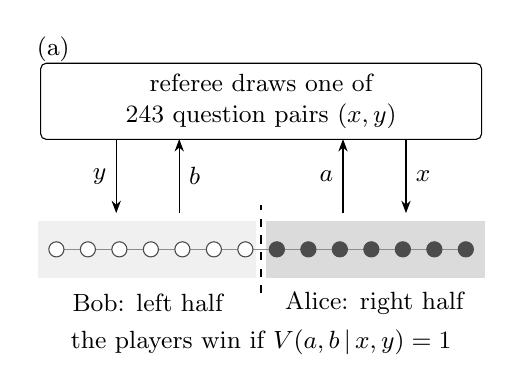
\begin{tikzpicture}[x=0.40cm,y=0.40cm,>={Stealth[length=4.5pt]},font=\small]
  \fill[black!6] (-7.1,-0.9) rectangle (-0.15,0.9);
  \fill[black!14] (0.15,-0.9) rectangle (7.1,0.9);
  \draw[black!45] (-6.5,0) -- (6.5,0);
  \foreach \i in {-6.5,-5.5,...,-0.5} \filldraw[fill=white,draw=black!70] (\i,0) circle (0.24);
  \foreach \i in {0.5,1.5,...,6.5} \filldraw[fill=black!70,draw=black!70] (\i,0) circle (0.24);
  \draw[dashed,thick] (0,-1.4) -- (0,1.4);
  \node at (-3.6,-1.7) {Bob: left half};
  \node at (3.6,-1.7) {Alice: right half};
  \node[draw,rounded corners=2pt,inner sep=4pt,align=center,minimum width=5.6cm] (ref) at (0,4.7)
       {referee draws one of\\ 243 question pairs $(x,y)$};
  \draw[->] (-4.6,3.5) -- node[left] {$y$} (-4.6,1.15);
  \draw[->] (-2.6,1.15) -- node[right] {$b$} (-2.6,3.5);
  \draw[->] (4.6,3.5) -- node[right] {$x$} (4.6,1.15);
  \draw[->] (2.6,1.15) -- node[left] {$a$} (2.6,3.5);
  \node[align=center] at (0,-2.95) {the players win if $V(a,b\,|\,x,y)=1$};
  \node at (-6.6,6.35) {(a)};
\end{tikzpicture}
\end{minipage}\hfill
\begin{minipage}[c]{0.46\textwidth}
\centering
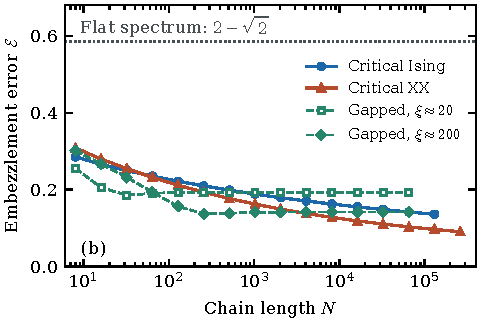
\includegraphics[width=\textwidth]{fig_main.pdf}
\end{minipage}
\caption{(a) The game. A chain in its ground state is cut in the middle, and each player
measures one half without communicating with the other. (b) Embezzlement error $\cE$ across
the cut. By Theorem~\ref{thm:equiv} the smallest losing probability lies between $\cE/C$ and
$(7/3)\,\cE$. For critical chains $\cE$ keeps decreasing as the chain grows, for gapped chains it
levels off after a few correlation lengths $\xi$, and for product states and Bell pairs it
stays at $2-\sqrt2$.}
\label{fig:main}
\end{figure}

\section{Setting}\label{sec:setting}

\subsection{Nonlocal games, bipartite systems and types}

A nonlocal game consists of finite sets of questions $x$ for Alice and $y$ for Bob, finite
sets of answers $a$ and $b$, a probability distribution $\pi(x,y)$ and a rule
$V(a,b\,|\,x,y)\in\{0,1\}$. The referee draws $(x,y)$ from $\pi$; the players, who cannot
communicate, answer $a$ and $b$ and win if $V(a,b\,|\,x,y)=1$~\cite{CHTW04,BrunnerRMP}.

\emph{Finite systems.} Let $\psi\in\cH_A\otimes\cH_B$ be a unit vector. A strategy assigns to
each question a positive operator-valued measure (POVM), $\{A^x_a\}_a$ on $\cH_A$ and
$\{B^y_b\}_b$ on $\cH_B$. Its losing probability is $\ip{\psi}{L\psi}$ with the loss operator
\begin{equation}\label{eq:loss}
L=\sum_{x,y}\pi(x,y)\sum_{a,b\,:\,V(a,b|x,y)=0}A^x_a\otimes B^y_b,\qquad 0\le L\le 1 ,
\end{equation}
and the value of the game at $\psi$ is $\omega(\psi)=1-\inf\ip{\psi}{L\psi}$, the infimum being
over all strategies. Local ancillas in fixed pure states are included, since a measurement on
system plus ancilla is a POVM on the system.

\emph{Infinite systems.} The Hilbert space of an infinite system need not factorize. A bipartite
system is then a pair of von Neumann algebras $M_A$, $M_B$ on a separable Hilbert space $\cH$
that commute, $M_B\subseteq M_A'$, together with a unit vector
$\Omega\in\cH$. Haag duality is the stronger equality $M_B=M_A'$. Alice's POVMs are taken in $M_A$ and Bob's in $M_B$, the product
$A^x_a\otimes B^y_b$ in~\eqref{eq:loss} is replaced by $A^x_aB^y_b$, and $\omega(\Omega)$ is
defined as before. For $M_A=\mathcal{B}(\cH_A)\otimes 1$ and $M_B=M_A'$ this is the tensor-product definition. For a pure
state of a spin chain with quasi-local algebra $\fA=\fA_L\otimes\fA_R$ (left and right
half-chains) and GNS representation $(\pi,\cH,\Omega)$ we put $M_A=\pi(\fA_R)''$ and
$M_B=\pi(\fA_L)''$.

\emph{Types.} A von Neumann algebra with trivial centre is a factor. A factor has type I if it
is isomorphic to all bounded operators on a Hilbert space, type II if it is not of type I but
has a faithful normal semifinite trace, and type III otherwise. For a faithful normal state
$\varphi=\ip{\Omega}{\,\cdot\,\Omega}$ on $M$, use the cyclic GNS space $\overline{M\Omega}$,
where $\Omega$ is also separating. Tomita--Takesaki theory provides the modular operator
$\Delta_\varphi$ on this space and the modular group
$\sigma_t^\varphi(x)=\Delta_\varphi^{it}x\Delta_\varphi^{-it}$; the fixed points of
$\sigma^\varphi$ form the centralizer $M_\varphi=\{x:\varphi(xy)=\varphi(yx)\ \forall y\}$. For $M=\mathcal{B}(\cH_A)$ with a faithful density matrix of eigenvalues
$p_j>0$, the modular point spectrum consists of the ratios $p_i/p_j$; the
full spectrum is their closure. Connes's invariant $S(M)$ is the intersection
of modular spectra over faithful normal semifinite weights. It is $\{1\}$
for semifinite factors, $\{0,1\}$ for III$_0$,
$\{0\}\cup\lambda^{\Z}$ for III$_\lambda$, $0<\lambda<1$, and
$[0,\infty)$ for III$_1$~\cite{Connes73,TakesakiII}.

\subsection{The game}\label{sec:game}

The game $\GIII$ is the game called $G_{\mathrm{III}}$ in Ref.~\cite{TG}, and
Appendix~\ref{app:game} reproduces its definition. It is built from nine copies of the flagged
magic-square game of Man\v{c}inska~\cite{Mancinska26}, which extends the Mermin--Peres
magic-square game~\cite{Mermin90,Peres90} by one extra answer, called a flag, and two extra
questions per player. One further question to Bob, whose answer is a label in $\Z/9\Z$, links
the nine copies. Alice has 45 possible questions and Bob 46, each with at most nine answers,
and the 243 question pairs that occur are asked with equal probability.

If either local algebra admits a faithful normal semifinite trace, then every strategy
loses with positive probability~\cite[Theorem~1.1]{TG}. For a factor $M_A$ with separable
predual in standard form, the same theorem characterizes the existence of a normal state
with a perfect strategy on $(M_A,M_A')$ by an invariant normal state on the flow of weights.
Every type-III$_1$ factor meets that criterion. The robust lower comparison in
Theorem~\ref{thm:equiv} uses Ref.~\cite[Theorem~1.4]{TG}, with an explicit constant proved in
Appendix~\ref{sec:explicit-robust}.
For CHSH on a standard pair, van Luijk, Stottmeister, Werner and Wilming obtained
$\beta\ge 2\sqrt{2}-8\sqrt{\kappa(\varphi)}$, where $\beta$ is the CHSH correlation
coefficient and $\kappa$ is their worst-case marginal error in predual
norm~\cite[Theorem~J and Proposition~100]{vLSWW24}.

\begin{lemma}[Linked modular bridge]
\label{lem:linked-bridge}
Let $M_A,M_B$ be commuting von Neumann algebras on $\cH$ and $\Omega$ a unit vector
whose marginal $\varphi$ on $M_A$ is faithful. Suppose that POVMs in these algebras
win $\GIII$ with probability one at $\Omega$. For each $j\in\Z/9\Z$, let $F_j$ be
Alice's flag effect on $R_1^j$. The $F_j$ are orthogonal projections in the centralizer
of $\varphi$, with $\sum_jF_j=1$ and $\varphi(F_j)=1/9$. There are partial isometries
$w_j\in M_A$ such that, for all real $t$,
\begin{equation}\label{eq:bridge}
w_j^*w_j=F_j,\qquad w_jw_j^*=F_{j+1}+F_{j+2},\qquad \sigma^\varphi_t(w_j)=2^{it}w_j .
\end{equation}
\end{lemma}

\begin{proof}
Let $e$ project onto $\overline{M_A\Omega}$. This space reduces $M_A$, and the
representation there is faithful and normal. Compress Bob's effects to it by
$B\mapsto eBe|_{e\cH}$. They still form POVMs in the commutant, and every expectation
$\ip{\Omega}{AB\Omega}$ is preserved because $e\Omega=\Omega$ and $[e,A]=0$.
We work in this cyclic and separating representation of the faithful normal state
$\varphi$~\cite[Lemma~1.6]{TG}.

A perfect binary match of commuting effects $P,Q$ has zero expectation of
$(P-Q)^2+P(1-P)+Q(1-Q)$. Positivity gives $P\Omega=Q\Omega$, and faithfulness
makes Alice's effect $P$ a projection. Replacing $P\Omega$ by $Q\Omega$ and commuting
$Q$ past $X\in M_A$ gives $\varphi(PX)=\varphi(XP)$. The first label test therefore
gives centralizer projections $F_j$ with $F_j\Omega=B_j^{\mathrm{Lab}}\Omega$.
The label effects sum to one, so separation gives $\sum_jF_j=1$ and the $F_j$ are
orthogonal. The second label test matches Alice's $R_2^j$ outcome $+++$ to
$B_{j+1}^{\mathrm{Lab}}+B_{j+2}^{\mathrm{Lab}}$. On $\Omega$ this sum equals
$F_{j+1}+F_{j+2}$, so separation identifies Alice's outcome with that
projection~\cite[Section~2.4]{TG}.

Each copy is a perfect flagged magic-square strategy on this faithful normal support.
The checked square generates a centralizer copy of $M_4$ with unit $1-F_j$, and the four
nonflag outcomes of $R_2^j$ are rank-one projections in it~\cite[Lemma~2.1]{TG}.
The calibrated sign tests give a partial isometry $\beta_j$ from $F_j$ onto a rank-one
projection $q_j$ of that copy, with $\sigma_t^\varphi(\beta_j)=2^{it}\beta_j$~\cite[Lemma~2.2]{TG}.
Choose a partial isometry $v_j$ in that matrix algebra with initial projection $q_j$
and final projection $F_{j+1}+F_{j+2}$. Then $w_j=v_j\beta_j$ has the required initial
and final projections, and $\sigma_t^\varphi(w_j)=v_j\sigma_t^\varphi(\beta_j)$ gives the
last identity in~\eqref{eq:bridge}. The KMS identity gives
$2\varphi(F_j)=\varphi(F_{j+1})+\varphi(F_{j+2})$.
A largest weight forces both successors to be largest, so all nine weights are $1/9$.
\end{proof}

For a nonfaithful marginal with support $p\in M_A$, the bridge applies in the corner
$pM_Ap$ on $p\cH$. The equality $p\Omega=\Omega$ and commutation of $p$ with Bob's effects
preserve the correlations in this reduction. On the standard pair of a faithful marginal,
the maps $s_r=\sum_j w_j^*F_{j+r}$ for $r=1,2$ satisfy $s_r^*s_s=\delta_{rs}1$,
$\sum_rs_rs_r^*=1$ and $\sigma_t^\varphi(s_r)=2^{-it}s_r$. The local column isometries
with entries $s_r^*$ and $Js_r^*J$, where $J$ is the modular conjugation, extract a Bell
pair exactly. Indeed, Tomita's identity gives
$s_r^*(Js_s^*J)\Omega=2^{-1/2}s_r^*s_s\Omega=2^{-1/2}\delta_{rs}\Omega$.

\subsection{The embezzlement error}\label{sec:E}

For a unit vector $\psi\in\cH_A\otimes\cH_B$ the embezzlement error $\cE(\psi)$ is defined by
the infimum in~\eqref{eq:E}, taken over unitaries $U_A$ on $\cH_A\otimes\C^2$ and $U_B$ on
$\cH_B\otimes\C^2$; $\Phi_2=(\ket{00}+\ket{11})/\sqrt2$ is a Bell pair on the two added qubits.
This is embezzlement in the sense of van Dam and Hayden with $\psi$ as the catalyst, measured
by the squared distance; the maximal overlap, or root fidelity, is $1-\cE/2$. Let
$\lambda=(\lambda_j)_{j\ge1}$, $\lambda_j=\sqrt{p_j}$, be the decreasing sequence of Schmidt
coefficients of $\psi$, and define an isometry $D$ on $\ell^2(\N)$ by
\begin{equation}\label{eq:D}
(D\lambda)_{2j-1}=(D\lambda)_{2j}=\lambda_j/\sqrt2 .
\end{equation}

\begin{lemma}[Formula for the embezzlement error]\label{lem:formula}
$\cE(\psi)=\norm{\lambda-D\lambda}^2=2-\sqrt2\sum_{m\ge1}\sqrt{p_m\,p_{\lceil m/2\rceil}}$.
\end{lemma}

\begin{proof}
The Schmidt coefficients of $\psi\otimes\ket{00}$ are $\lambda$, and those of
$\psi\otimes\Phi_2$ are $D\lambda$, which is again decreasing. For two unit vectors with
decreasing Schmidt coefficients $\alpha$ and $\beta$, the supremum of the overlap
$\lvert\ip{\chi}{(U_A\otimes U_B)\chi'}\rvert$ over local unitaries is $\sum_j\alpha_j\beta_j$.
This is von Neumann's trace inequality~\cite{HornJohnson}; the bound is attained by aligning
the Schmidt bases in finite dimensions and approached in infinite dimensions. Hence the infimum
in~\eqref{eq:E} equals $2-2\ip{\lambda}{D\lambda}=\norm{\lambda-D\lambda}^2$, because $D$ is an
isometry.
\end{proof}


For a target of dimension $d$ the same argument gives
\begin{equation}\label{eq:Ed}
\cE_d(p)=\|(1-D_d)\lambda\|_2^2,
\qquad (D_d\lambda)_j=d^{-1/2}\lambda_{\lceil j/d\rceil}.
\end{equation}
The distinction between local-unitary and LOCC error matters for rates;
we use~\eqref{eq:Ed} throughout.


\section{The sharp chain law}\label{sec:law}

Theorems~\ref{thm:xx-full-law} and~\ref{cor:ising-full-law} concern the exact finite spectra. Their common mechanism is a smooth limit of logarithmic Schmidt rank, with quantitative control of every spectral plateau. We first prove a criterion that isolates this mechanism.

\paragraph{Energy counts and logarithmic rank.}
Consider a family of spectra written as $p_\nu=e^{-L(1)-A_\nu}$,
where $A_\nu\ge0$ are energies listed with multiplicity and
$L(z)=\log\sum_\nu e^{-z A_\nu}$ is the logarithm of the partition
function. Under the tilted law $p_{\beta,\nu}=e^{-L(\beta)-\beta A_\nu}$,
the mean and variance of $A$ are $m_\beta=-L'(\beta)$ and
$v_\beta=L''(\beta)$. In particular $V=v_1$ is the information
variance of the original spectrum. Let $W\to\infty$ index the family.

\begin{proposition}[A counting criterion for the embezzlement law]
\label{prop:xx-count-to-error}
Suppose $L$ is analytic on a fixed complex neighborhood of a fixed
real interval $[1-\eta,1+\eta]\subset(0,\infty)$, with
$|L^{(k)}(z)|\le C_k W$ for each fixed $k\ge1$, and $v_\beta\ge cW$
on the real interval. Suppose the tilted characteristic functions
$\varphi_\beta(t)=\mathbb E_\beta e^{itA}$ obey, uniformly in that interval,
\begin{equation}\label{eq:chain-damping}
 |\varphi_\beta(t)|\le
 \begin{cases}
 e^{-cWt^2}, & |t|\le\delta,\\
 e^{-cW}, & \delta\le |t|\le\tau W,
 \end{cases}
\end{equation}
for positive constants $c,\delta,\tau$ independent of $W$. Then, for all
integers $d\ge2$, with $h=\log d$,
\begin{equation}\label{eq:xx-error-capacity}
 \left|\mathcal E_d-\frac{h^2}{4V}\right|
 \le\frac{C(1+h^2+h^4)}{W^2}.
\end{equation}
Here $C$ and the large-$W$ threshold are independent of $d$.
\end{proposition}

\begin{proof}
Write $R(E)=\#\{\nu:A_\nu\le E\}$ and
$R(E^-)=\#\{\nu:A_\nu<E\}$. Set $\mu=m_1$ and $B=\sqrt W\log W$.
For $|E-\mu|\le2B$, let $\beta(E)$ solve $m_\beta=E$. Since
$m_\beta'=-v_\beta$ has magnitude of order $W$, this solution is unique
and lies in the given interval for large $W$. Define
\begin{equation}\label{eq:xx-saddle-F}
 F(E)=L(\beta(E))+\beta(E)E-\log\beta(E)
      -\tfrac12\log(2\pi v_{\beta(E)}).
\end{equation}
Lemma~\ref{lem:xx-microscopic-counting} in Appendix~\ref{app:xx-full}
gives the uniform estimate for $|E-\mu|\le2B$,
\begin{equation}\label{eq:xx-microscopic-counting}
 \log R(E)=F(E)+O(W^{-1}),\qquad
 \log R(E^-)=F(E)+O(W^{-1}).
\end{equation}
Indeed, with $\beta=\beta(E)$ the exact tilted count is
\[
 e^{-L(\beta)-\beta E} R(E)=\mathbb E_\beta
      \bigl[e^{-\beta(E-A)}\mathbf1_{\{A\le E\}}\bigr].
\]
The lemma uses both frequency bounds in~\eqref{eq:chain-damping} and
an even smoothing kernel with Fourier support in $[-\tau W,\tau W]$.
The tilted interval-probability estimate~\eqref{eq:xx-concentration}
bounds the change under smoothing and the mass of any atom at $E$
by $O(W^{-3/2})$. The analytic derivative bounds and $v_\beta\asymp W$
give the saddle-point value $(\beta\sqrt{2\pi v_\beta})^{-1}$ with
relative error $O(W^{-1})$ in the Fourier integral
\eqref{eq:xx-smoothed-fourier}.

Put $p(x)=p_{\lceil x\rceil}$ for the decreasing list of probabilities,
with zero padding for a finite list, and $g(y)=e^{y/2}\sqrt{p(e^y)}$.
If $E_x=-\log p(x)-L(1)$ is finite, then
$R(E_x^-)<x\le R(E_x)$. The two counts in
\eqref{eq:xx-microscopic-counting} give $\log x=F(E_x)+O(W^{-1})$
throughout each degenerate plateau in the counting window.
Since $F'(E)=\beta(E)+O(W^{-1})$ is bounded away from zero there,
its inverse $E_*(y)=F^{-1}(y)$ satisfies the energy
comparison~\eqref{eq:xx-inverse-rank} on
$F([\mu-3B/2,\mu+3B/2])$. Let $\chi$ be a smooth function equal to one
on $[-1,1]$ and supported inside $(-3/2,3/2)$, and define
\[
 G(y)=\chi\bigl((E_*(y)-\mu)/B\bigr)
        \exp\bigl((y-L(1)-E_*(y))/2\bigr)
\]
on the range of $F$, extended by zero. Lemma~\ref{lem:chain-rank-profile}
proves
\begin{equation}\label{eq:chain-profile-estimates}
 \norm{g-G}_2=O(W^{-1}),\qquad \norm{G''}_2=O(W^{-1}),\qquad
 \norm{G'}_2^2=\frac{1}{4V}+O(W^{-2}).
\end{equation}
The first estimate uses concentration under the original law to control
the full tail. The derivative estimates follow from the logarithmic
derivative $a(E)=1-1/F'(E)$ of the squared uncut profile. Its Taylor
coefficients about $\mu$ through degree two have orders
$O(W^{-1})$, $-1/V+O(W^{-2})$, and $O(W^{-2})$, respectively.
The first and third centered moments of the exact energy are $0$ and
$O(W)$, which controls the cross terms in the integral of $a^2$.

For $T_h g(y)=g(y-h)$ set $D_h=I-T_h$. The continuous rank coordinate
preserves the exact error $\mathcal E_d=\norm{D_hg}_2^2$ because
$p(x/d)=p_{\lceil j/d\rceil}$ almost everywhere on $(j-1,j]$.
Writing $r=g-G$, we have
\[
 \norm{D_hg}_2^2-\norm{D_hG}_2^2
   =2\operatorname{Re}\langle D_h^*D_hG,r\rangle+\norm{D_hr}_2^2.
\]
The multiplier of $D_h^*D_h=2I-T_h-T_{-h}$ is $2-2\cos(ht)$, bounded
by $h^2t^2$. Thus the last display is $O((1+h^2)W^{-2})$ by
\eqref{eq:chain-profile-estimates}. The same multiplier differs from
$h^2t^2$ by $O(h^4t^4)$, so
$\norm{D_hG}_2^2=h^2\norm{G'}_2^2+O(h^4\norm{G''}_2^2)$.
This proves~\eqref{eq:xx-error-capacity}.
\end{proof}

\paragraph{The exact covariance supplies the counting estimates.}
For the open XX chain let $C_N$ be the occupied one-particle projector
and write $C_N$ in blocks for the two halves. If $s_j$ are the singular
values of its cross block, then $s_j^2=\lambda_j(1-\lambda_j)$ as a
multiset, where $\lambda_j$ are the restricted covariance eigenvalues.
The Schmidt probabilities form a product of two-outcome distributions
with one-mode energies $e_j=2\operatorname{arcosh}(1/(2s_j))$.
With zero padding, Corollary~\ref{cor:xx-mesh} compares the ordered
$(s_j)$ in $\ell^1$ with error $O(1)$ to the mesh
\begin{equation}\label{eq:chain-main-mesh}
 \left\{\tfrac12\operatorname{sech}(2\pi^2 k/L_i)
                    :k\in\mathbb Z,\ i=1,2\right\},
 \qquad L_i=\log N+O(1).
\end{equation}
The two branches come from the two parity blocks of the exact sine
covariance. Each is compared with a finite Hilbert matrix, then with a
periodized Carleman kernel diagonal in Fourier modes.

This mesh gives $\sum_j s_j=O(\log N)$, which bounds the fixed-order
derivatives of $L(z)=\sum_j\log(1+e^{-ze_j})$ by $O(\log N)$ near
$\beta=1$. In any fixed positive energy band $[a,b]$, a mesh branch
has spacing $4\pi^2/L_i$. All but $O(1)$ entries in the band match
true energies in $[a/2,2b]$, with total absolute discrepancy $O(1)$.
These modes give $v_\beta\ge c\log N$. The Bernoulli characteristic
factor has squared modulus $1-4q(1-q)\sin^2(te_j/2)$, where
$q=(1+e^{\beta e_j})^{-1}$. For small $t$ the retained modes give a
sine-square sum of order $Wt^2$ with $W=\log N$. For $|t|\ge\delta$
the mesh sum is bounded below by $cW-O(1+|t|)$ by integral comparison.
Replacing the mesh energies by the matched true energies costs another
$O(1+|t|)$. Choosing $\tau$ sufficiently small yields
\eqref{eq:chain-damping} through $|t|\le\tau W$.

The entropy and information variance are sums over modes of
\[
 f_S(e)=\log(1+e^{-e})+\frac{e}{1+e^e},\qquad
 f_V(e)=\frac{e^2 e^e}{(1+e^e)^2}.
\]
As functions of $s=(2\cosh(e/2))^{-1}$ both are Lipschitz. The mesh
comparison therefore changes their sums by $O(1)$. The two mesh
branches give density $(L_1+L_2)/(2\pi^2)$ in positive energy and
$\int_0^\infty f_S(e)\,de=\int_0^\infty f_V(e)\,de=\pi^2/6$.
This gives~\eqref{eq:xx-three-limits} and recovers the open-boundary
entropy coefficient of Calabrese and Cardy and of Fagotti and
Calabrese for XX~\cite{CalabreseCardy04,FagottiCalabrese11}.
The matching leading term for $V$, the capacity of entanglement,
agrees with the conformal R\'enyi calculation~\cite{deBoer19,Arias23}.
Proposition~\ref{prop:xx-count-to-error} now gives
\eqref{eq:xx-full-rate} and~\eqref{eq:xx-full-limit}.

For Ising, the exact Majorana decomposition identifies the mode list of
the XX chain on $2L$ sites with two copies of the Ising list on $L$
sites (Corollary~\ref{cor:ising-fourier}). The Ising logarithmic partition
function is therefore half that of XX, and its tilted characteristic
function has modulus equal to the square root of the XX modulus. This
proves Corollary~\ref{cor:ising-full-law} with $W=\log L$.

\begin{corollary}[Loss of the explicit strategy]\label{cor:xx-strategy}
For the finite open XX and critical Ising states, the explicit
measurements of Theorem~\ref{thm:operational-upper} achieve
$\mathcal B(p)=(2/243)\mathcal E_2(1+o(1))$. The leading losses are
$(\log2)^2/(81\log N)$ for XX and $2(\log2)^2/(81\log L)$ for Ising.
\end{corollary}

\begin{proof}
The same mesh gives $b_N=-\log p_1\sim(\log N)/12$ for XX and
$b_L\sim(\log L)/24$ for Ising (Appendix~\ref{app:xx-full}). Thus
$p_1=o(\mathcal E_2)$, and the achieved loss follows from the
state-dependent estimate in Theorem~\ref{thm:operational-upper}.
\end{proof}

Corollary~\ref{cor:chain-arbitrary-cuts} extends the chain law uniformly
to cuts between any two adjacent sites in either open chain as the
shorter side grows. The logarithm of the shorter side sets the scale.
The corollary also covers Ising chains of odd length.

\begin{corollary}[Targets of growing dimension]\label{cor:chain-growing-target}
Under the assumptions of Proposition~\ref{prop:xx-count-to-error},
uniformly over integers $d\ge2$ as $W\to\infty$,
\begin{equation}\label{eq:chain-gaussian-crossover}
 \mathcal E_d=2\left(1-\exp\left[-\frac{(\log d)^2}{8V}\right]\right)+o(1).
\end{equation}
In particular the error tends to zero precisely when $\log d=o(\sqrt V)$.
In this regime the error is asymptotic to $(\log d)^2/(4V)$ by
\eqref{eq:xx-error-capacity}.
\end{corollary}

The optimal local-unitary root fidelity $1-\mathcal E_d/2$ has the
limiting Gaussian form proved for LOCC by Zhang, Liu and
Chen~\cite[Supplement, Theorem~1]{ZhangLiuChen26}. The counting criterion
establishes this form for the exact finite XX and Ising spectra.

\begin{proof}
Set $y_0=F(\mu)=L(1)+\mu-\tfrac12\log(2\pi V)$ and define the
probability density $\rho_W(z)=\sqrt V\,g(y_0+\sqrt V\,z)^2$.
For $y=y_0+\sqrt V\,z$ at fixed $z$, let $u=F^{-1}(y)-\mu$.
Since $F'$ is bounded away from zero, $u=O_z(\sqrt W)$.
The derivative bounds from Appendix~\ref{app:xx-full} give
\[
 F(\mu+u)-F(\mu)=u-\frac{u^2}{2V}
              +O\left(\frac{|u|}{W}+\frac{|u|^3}{W^2}\right).
\]
It follows that $u=\sqrt V\,z+O_z(1)$. By the inverse count estimate
\eqref{eq:xx-inverse-rank}, the exact energy at rank $e^y$ is
$\mu+u+O(W^{-1})$. Consequently
\[
 \log\rho_W(z)=-\tfrac12\log(2\pi)+y-y_0-u+O(W^{-1})
              \longrightarrow-\tfrac12\log(2\pi)-z^2/2.
\]
Both $\rho_W$ and the standard normal density $\phi$ integrate to one.
Dominated convergence applied to $\min(\rho_W,\phi)$ gives
$\norm{\rho_W-\phi}_1\to0$ and hence
$\norm{\sqrt{\rho_W}-\sqrt\phi}_2\to0$. Translation by $h$ in $y$
becomes translation by $h/\sqrt V$ in $z$. Since $\norm{I-T_a}\le2$
uniformly in real $a$, the squared translation errors of the two
square-root densities differ by $o(1)$ uniformly in the shift.
The Gaussian overlap is
$\langle\sqrt\phi,T_a\sqrt\phi\rangle=e^{-a^2/8}$, which gives
\eqref{eq:chain-gaussian-crossover}.
\end{proof}

\subsection{Exact discrete towers}

For an end block of a critical chain, conformal field theory describes the
reduced state through an annulus Hamiltonian. Its width grows as
$W=\ln(\kappa N)$ and its level degeneracies depend on the boundary
operator content~\cite{PeschelEisler09,Lauchli13,CardyTonni16,ACT18}.
For the corresponding open-boundary conformal comparison, the free-fermion
towers have odd one-body levels
\begin{equation}\label{eq:levels}
\varepsilon_\ell=(2\ell+1)\varepsilon,\qquad
\varepsilon=\pi^2/W,
\end{equation}
once for Ising and twice for XX~\cite{IgloiJuhasz08}. The double odd tower
is the comparison for the XX sizes divisible by four used in the numerical
study. When $N/2$ is odd, the finite XX covariance has an exact $1/2$ mode,
which contributes a flat Schmidt factor. The finite-chain theorem
covers both parity sectors. Such towers also occur
as exact half-chain spectra in integrable gapped models~\cite{PKL99}.
For the towers themselves, the leading embezzlement law can be proved
without replacing the discrete levels by a smooth density.
For a fixed integer $r\geq1$ and $\varepsilon>0$, consider the normalized
countable spectrum
\begin{equation}\label{eq:tower-spectrum-rigorous}
 p_{\boldsymbol\nu}=Z_r(\varepsilon)^{-1}
 \exp\!\left[-\varepsilon
   \sum_{a=1}^{r}\sum_{\ell\geq0}(2\ell+1)\nu_{a,\ell}\right],
 \qquad
 Z_r(\varepsilon)=\prod_{\ell\geq0}
       (1+e^{-(2\ell+1)\varepsilon})^r .
\end{equation}
Here every $\nu_{a,\ell}$ is $0$ or $1$ and only finitely many occupations
are nonzero.  Order the probabilities decreasingly as $(p_j)_{j\geq1}$,
put $\lambda_j=\sqrt{p_j}$, and define
\[
 (D_d\lambda)_j=d^{-1/2}\lambda_{\lceil j/d\rceil},
 \qquad
 \mathcal E_d=\norm{\lambda-D_d\lambda}_2^2,
 \qquad S=-\sum_j p_j\log p_j .
\]
The cases $r=1,2$ are the single and double odd-level towers used for
the Ising and XX conformal spectra, respectively.

\begin{theorem}[Exact discrete tower law]\label{thm:exact-tower-law}
Fix integers $r\geq1$ and $d\geq2$, and set
$c_r=r\pi^2/24$.  For the exact spectrum
\eqref{eq:tower-spectrum-rigorous}, as $\varepsilon\downarrow0$,
\begin{align}
 S&=\frac{2c_r}{\varepsilon}+O_r(\varepsilon),
 \label{eq:tower-entropy-rigorous}\\
 \mathcal E_d
 &=\frac{(\log d)^2\varepsilon}{8c_r}
       +O_{r,d}(\varepsilon^2),
 \label{eq:tower-error-rigorous}\\
 \mathcal E_d S&=\frac{(\log d)^2}{4}
       +O_{r,d}(\varepsilon).
 \label{eq:tower-product-rigorous}
\end{align}
All constants are independent of $\varepsilon$. The left-hand sides use
the exact discrete spectrum with its full level multiplicities.
\end{theorem}


Appendix~\ref{app:tower} proves the tower law by applying
Proposition~\ref{prop:xx-count-to-error} to the exact spectrum with
$W=\varepsilon^{-1}$. The tilted characteristic-function
bound~\eqref{eq:characteristic-tail} for the integer tower levels
gives~\eqref{eq:chain-damping} after rescaling to the physical energy
spacing. This yields the $O_{r,d}(\varepsilon^2)$ remainder.
Lemma~\ref{lem:tower-uniform-comparison} also compares the exact tower
with the smooth Calabrese--Lefevre distribution in Hellinger distance.


\subsection{Numerical comparison}
For target dimension two, write $\cE_{\mathrm{tower}}^{(r)}(b)$ for the
$r$-copy tower curve at $b=-\ln p_1$, and $\cE_{\mathrm{s}}(b)$ for
the smooth Calabrese--Lefevre curve. The tower superscript labels level
multiplicity; the subscript $d$ in $\cE_d$ always labels the target dimension.

\begin{figure}[t]
\centering
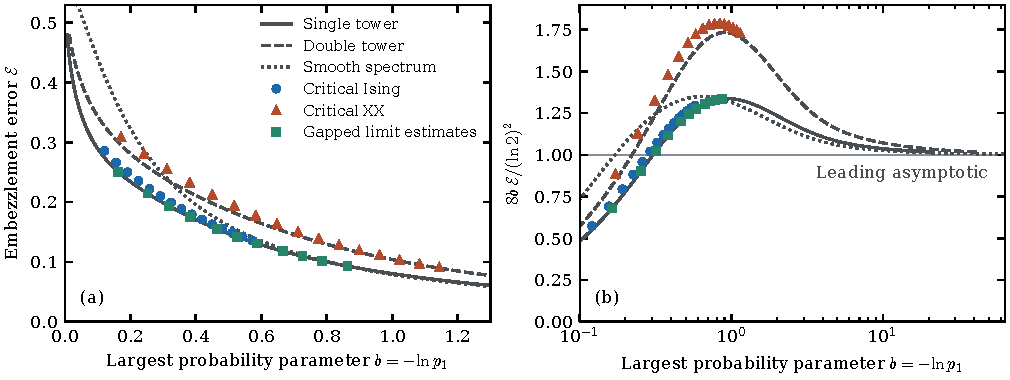
\includegraphics[width=\textwidth]{fig_law.pdf}
\caption{The finite-size law. (a) Embezzlement error against $b=-\ln p_1$ for the critical Ising
chain ($8$ to $131{,}072$ spins), the critical XX chain ($8$ to $262{,}144$ sites) and gapped
chains in the limit of long chains. Curves: prediction from equally spaced entanglement
levels~\eqref{eq:levels}, each level occurring once or twice, and from the smooth conformal
spectrum of Ref.~\cite{CalabreseLefevre08}. (b) The same data and curves multiplied by
$8b/(\ln2)^2$. The proved XX, Ising and tower asymptotics correspond to the value one; it is approached
slowly.}
\label{fig:law}
\end{figure}

\paragraph{Test.} We computed the entanglement spectra of the ground states of three chains by
the correlation-matrix method~\cite{Peschel03,VLRK03}: the critical XX chain with open ends, the
critical transverse-field Ising chain with open ends, and the XX chain with a staggered
potential, which is gapped with correlation length $\xi$. All chains are cut in the middle.
Appendix~\ref{app:numerics} gives the methods and checks. Figures~\ref{fig:main}(b)
and~\ref{fig:law} and Table~\ref{tab:chains} show the results.

\begin{table}[t]
\centering\small
\begin{tabular}{@{}llccccc@{}}
\toprule
 & & $S$ & $b$ & $\cE$ & $\cE/\cE_{\mathrm{tower}}^{(r)}(b)$ & $\cE/\cE_{\mathrm{s}}(b)$\\
\midrule
Critical Ising & $N=16$ & 0.423 & 0.156 & 0.2663 & 1.049 & 0.72 \\
 & $N=256$ & 0.663 & 0.292 & 0.2100 & 1.043 & 0.84 \\
 & $N=4{,}096$ & 0.895 & 0.419 & 0.1708 & 1.030 & 0.91 \\
 & $N=65{,}536$ & 1.126 & 0.542 & 0.1420 & 1.022 & 0.95 \\
 & $N=131{,}072$ & 1.184 & 0.572 & 0.1361 & 1.021 & 0.96 \\
\addlinespace
Critical XX & $N=16$ & 0.714 & 0.241 & 0.2799 & 1.065 & 0.97 \\
 & $N=256$ & 1.210 & 0.518 & 0.1935 & 1.065 & 1.24 \\
 & $N=4{,}096$ & 1.674 & 0.775 & 0.1382 & 1.038 & 1.33 \\
 & $N=65{,}536$ & 2.136 & 1.022 & 0.1034 & 1.020 & 1.34 \\
 & $N=262{,}144$ & 2.367 & 1.144 & 0.0908 & 1.015 & 1.34 \\
\addlinespace
Staggered XX & $\xi=20$ & 0.729 & 0.318 & 0.1932 & 1.000 & 0.82 \\
 & $\xi=200$ & 1.114 & 0.526 & 0.1420 & 1.000 & 0.93 \\
 & $\xi=2{,}000$ & 1.498 & 0.726 & 0.1092 & 1.000 & 0.98 \\
 & $\xi=10{,}000$ & 1.766 & 0.864 & 0.0929 & 1.000 & 1.00 \\
\bottomrule
\end{tabular}
\caption{Entanglement entropy $S$, $b=-\ln p_1$ and embezzlement error $\cE$ of half-chain
ground states. $\cE_{\mathrm{tower}}^{(1)}$ (Ising and gapped chains) and $\cE_{\mathrm{tower}}^{(2)}$ (XX chain) are the predictions from
equally spaced levels at the same $b$; $\cE_{\mathrm{s}}$ is the prediction of the smooth
conformal spectrum. For gapped chains the values estimate the long-chain limits.}\label{tab:chains}
\end{table}

In both critical chains $\cE$ decreases monotonically over the sampled
powers of two, spanning more than four decades in size. At the larger
sizes, the increments in $1/\cE$ grow with successive doublings.
The slope of $S$ with respect to $\ln N$ at the largest sampled
doubling is $0.083335$ for Ising and $0.166670$ for XX, close to $c/6$
for $c=1/2$ and $c=1$, respectively.

The spectra have the predicted form. For the gapped chain the one-body entanglement energies
satisfy $\varepsilon_\ell/\varepsilon_0=2\ell+1$ to five digits, and $\cE$ agrees with $\cE_{\mathrm{tower}}^{(1)}(b)$
within $2\times10^{-4}$ for all $\xi$ from $4$ to $10^4$. At criticality the levels are equally
spaced only approximately. For the Ising chain, expressing $\varepsilon_0$
as $\pi^2/\ln(\kappa N)$ gives $\kappa=16.9$ at $1{,}024$ spins and
$17.6$ at $131{,}072$ spins. The ratios
$\varepsilon_\ell/\varepsilon_0$ for $\ell=1,2,3$ are $3.13$, $5.46$ and $7.95$
at $1{,}024$ spins and $3.04$, $5.18$ and $7.39$ at $131{,}072$ spins.
Accordingly $\cE/\cE_{\mathrm{tower}}^{(1)}(b)$ falls from $1.05$ to $1.021$ for the Ising chain, and
$\cE/\cE_{\mathrm{tower}}^{(2)}(b)$ falls from $1.07$ to $1.015$ for the XX chain.

The comparison with the smooth spectrum shows which conformal data matter. At fixed $b$ the smooth spectrum is a one-parameter approximation that suppresses tower degeneracies, and at the largest sizes the XX chain lies $34\%$ above it
while the Ising chain lies $4\%$ below. What distinguishes $\cE_{\mathrm{tower}}^{(1)}$, $\cE_{\mathrm{tower}}^{(2)}$ and
$\cE_{\mathrm{s}}$ is the operator content, that is, the degeneracies of the levels of $L_0$.

The sampled chains remain pre-asymptotic for $\cE$. At $N=4{,}096$,
the XX chain gives $\cE\simeq0.13824$ and $V\simeq1.58147$.
The error is about $82\%$ above the capacity expression
$(\ln2)^2/(4V)\simeq0.07595$ and about $60\%$ above the leading
logarithmic expression $3(\ln2)^2/(2\ln N)\simeq0.08664$ in
\eqref{eq:xx-full-rate}.
The combination $8b\,\cE/(\ln2)^2$, which tends to one under
Theorem~\ref{thm:xx-full-law}, still equals $1.19$, $1.08$ and
$1.016$ at $b=2$, $4$ and $16$ for the smooth spectrum, and $1.14$ and $1.27$ at $b=3.2$ on the
curves $\cE_{\mathrm{tower}}^{(1)}$ and $\cE_{\mathrm{tower}}^{(2)}$.
The Ising and XX samples reach $b=0.57$ and $b=1.14$, respectively.
On the large-$S$ side of Figure~\ref{fig:diagnostics}(a), the
entropy-normalized error comes within ten per cent of one near
$S\simeq7$ for the smooth curve and near $S\simeq9$ and $S\simeq15$
for the single and double towers.

Gapped chains behave like critical chains of finite length. Their $\cE$ stops decreasing once
$N$ exceeds a few correlation lengths (Figure~\ref{fig:main}(b)). The estimated limiting value lies close to
the curve $\cE_{\mathrm{tower}}^{(1)}(b)$ and falls slowly with $\xi$, from $0.193$ at $\xi=20$ to $0.142$, $0.109$
and $0.093$ at $\xi=200$, $2{,}000$ and $10{,}000$.


\begin{figure}[t]
\centering
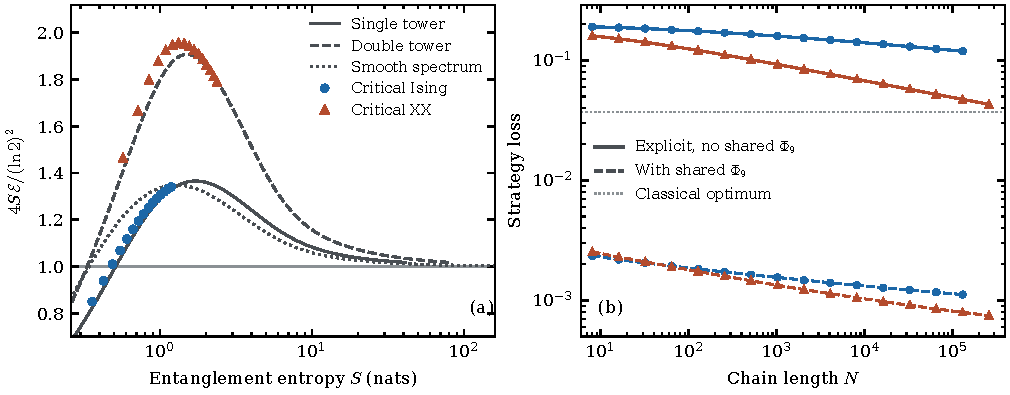
\includegraphics[width=\textwidth]{fig_diagnostics.pdf}
\caption{(a) The entropy-normalized error for the physical chains, exact
towers and smooth spectrum. The exact tower and finite-chain theorems give limit one.
(b) The exact loss of the explicit unassisted strategy (solid) and the
loss after adding $\Phi_9$ (dashed). The horizontal line is the classical
optimum $1/27$. These are achieved strategy losses, not values of the
optimization over all measurements.}\label{fig:diagnostics}
\end{figure}

At the largest sizes the explicit unassisted losses are $0.11895$ for Ising
and $0.04295$ for XX, both above the classical loss $1/27$.
With the additional $\Phi_9$, the losses are $1.120\times10^{-3}$ and
$7.472\times10^{-4}$. These achieved losses lie below the classical bound and above the flat-spectrum
floor $\gamma$. The compressed certificate of
Section~\ref{sec:xx84-separation} establishes separation in the original
game at the explicit larger length $N=2^{84}$.
Section~\ref{sec:finite-chain-hybrid} gives an exact four-spin separation
using a tagged extension, and Section~\ref{sec:operational-lower} gives
a nine-qubit resource separated by the original game.


\section{The game measures the embezzlement error}\label{sec:equiv}

We first collect the properties of $\cE$ that are used below. The
bounds~\eqref{eq:window}--\eqref{eq:variance} are contained in Ref.~\cite[Section~6.4]{TG}, and
we include short proofs to keep the paper self-contained. Throughout, $T$ denotes a random
variable on $(0,\infty)$ with density $p(t)=p_{\lceil t\rceil}$, which is a continuous version
of the rank of a Schmidt probability, and $X=\log_2T$.

\begin{proposition}[Properties of $\cE$]\label{prop:E}
Let $\psi$ be a pure bipartite state with Schmidt probabilities $p_1\ge p_2\ge\cdots$, Schmidt
coefficients $\lambda$ and entanglement entropy $S=-\sum_jp_j\ln p_j\le\infty$. The embezzlement
error is positive and never exceeds its value on a product state,
\begin{equation}\label{eq:range}
0<\cE(\psi)\le2-\sqrt2,
\end{equation}
with equality on the right exactly when all nonzero $p_j$ are equal, that is, for product
states and maximally entangled states. It does not change when a maximally entangled state
$\Phi_k$ of any local dimension $k$ is added, and its square root is Lipschitz continuous in the
Schmidt coefficients: if $\psi'$ has Schmidt coefficients $\lambda'$, then
\begin{equation}\label{eq:invariance}
\cE(\psi\otimes\Phi_k)=\cE(\psi),\qquad
\bigl\lvert\sqrt{\cE(\psi)}-\sqrt{\cE(\psi')}\bigr\rvert\le2\norm{\lambda-\lambda'}.
\end{equation}
A small error forces the Schmidt probabilities to spread over many ranks. The largest of them,
and the total weight of the ranks between $r+1$ and $2r$ for every integer $r\ge1$, satisfy
\begin{equation}\label{eq:window}
p_1\le(6+4\sqrt2)\,\cE(\psi),\qquad\sum_{j=r+1}^{2r}p_j\le\sqrt{\cE(\psi)} ,
\end{equation}
while the entanglement entropy and, when finite, the variance of $X$ satisfy
\begin{equation}\label{eq:entropybound}
\sqrt{\cE(\psi)}\;\ge\;\frac{\ln2}{2\,(S+1+3\ln2)}
\end{equation}
and
\begin{equation}\label{eq:variance}
\cE(\psi)\,\bigl(4\Var(X)+1\bigr)\ge1 .
\end{equation}
\end{proposition}

\begin{proof}
We use the formula $\cE=\norm{\lambda-D\lambda}^2=2-2\ip{\lambda}{D\lambda}$ of
Lemma~\ref{lem:formula} throughout.

\emph{Range.} Since $\lambda$ is decreasing, $\lambda_{\lceil m/2\rceil}\ge\lambda_m$. Hence
$\ip{\lambda}{D\lambda}=\sum_m\lambda_m\lambda_{\lceil m/2\rceil}/\sqrt2\ge1/\sqrt2$, which is
the upper bound in~\eqref{eq:range}. Equality requires
$\lambda_m\in\{0,\lambda_{\lceil m/2\rceil}\}$ for all $m$, that is, a flat spectrum. Positivity
follows from the first bound in~\eqref{eq:window}.

\emph{Invariance and continuity.} The Schmidt coefficients of $\psi\otimes\Phi_k$ are
$(D_k\lambda)_m=\lambda_{\lceil m/k\rceil}/\sqrt k$. The map $D_k$ is an isometry, and it
commutes with $D=D_2$ because $\lceil\lceil m/k\rceil/2\rceil=\lceil m/(2k)\rceil$. Therefore
$\norm{D_k\lambda-DD_k\lambda}=\norm{D_k(\lambda-D\lambda)}=\norm{\lambda-D\lambda}$. The
Lipschitz bound holds because $\sqrt{\cE}=\norm{(1-D)\lambda}$ and $\norm{1-D}\le2$.

\emph{Largest probability and windows.} The first component of $\lambda-D\lambda$ is
$\lambda_1(1-1/\sqrt2)$, so $\cE\ge p_1(1-1/\sqrt2)^2=p_1/(6+4\sqrt2)$. For the second bound
in~\eqref{eq:window}, let $f(s)=(\ln2)\,2^sp(2^s)$ be the density of $X$ and $g=\sqrt f$. The
substitution $t=2^{s+1}$ in
$\norm{\lambda-D\lambda}^2=\int_0^\infty\bigl(\sqrt{p(t)}-\sqrt{p(t/2)/2}\bigr)^2dt$ gives
\begin{equation}\label{eq:Eshift}
\cE(\psi)=\int_{\R}\bigl(g(s+1)-g(s)\bigr)^2\,ds .
\end{equation}
In other words, the embezzlement error measures how much the distribution of $X$ changes when
it is shifted by one. Put $\mu(u)=\int_u^{u+1}f$. By the Cauchy--Schwarz inequality,
$\sum_{k\in\Z}\lvert\mu(u+k)-\mu(u+k-1)\rvert\le\int_{\R}\lvert g(s)-g(s-1)\rvert\,(g(s)+g(s-1))\,ds\le2\sqrt{\cE}$.
The left-hand side is the total variation of a nonnegative summable sequence and is therefore
at least twice its maximum. So $\mu(u)\le\sqrt{\cE}$ for all $u$, and the choice $u=\log_2r$
gives the claim.

\emph{Entropy.} Because $p$ is decreasing, $t\,p(t)\le\int_0^tp\le1$, hence
$-\ln p(T)\ge\ln T$ and $S\ge(\ln2)\,\mathbb{E}[X]$. The negative part of $X$ contributes
$\int_0^1p_1\log_2(1/t)\,dt=p_1/\ln2\le1/\ln 2$. Put $h=\sqrt{\cE}$. For $x\ge0$ the interval
$(1,2^x]$ is covered by at most $x+1$ windows of the form $(r,2r]$, and $p_1=2\mu(-1)\le2h$, so
$\Pr[X\le x]\le(x+3)h$ and
$\mathbb{E}[X_+]\ge\int_0^\infty(1-(x+3)h)_+\,dx=(1-3h)_+^2/(2h)$. If $h<1/3$ this gives
$S\ge(\ln2)\bigl(\tfrac1{2h}-3\bigr)-1$, which is~\eqref{eq:entropybound}. If $h\ge1/3$
then~\eqref{eq:entropybound} holds because its right-hand side is below $0.12$.

\emph{Variance.} Assume $X$ has finite second moment; otherwise the variance bound is interpreted as vacuous. The laws of $X$ and $X-1$ have means that differ by one. With
$\mu_X=\mathbb{E}[X]$ and $c=\mu_X-\tfrac12$ we obtain
$1=\int(s-c)\bigl(f(s)-f(s+1)\bigr)ds\le\sqrt{\cE}\,\bigl(\norm{(s-c)g(s)}_2+\norm{(s-c)g(s+1)}_2\bigr)
=2\sqrt{\cE}\,\sqrt{\Var(X)+\tfrac14}$, which is~\eqref{eq:variance}.
\end{proof}

\begin{remark}\label{rem:sharp}
The power of $S$ in~\eqref{eq:entropybound} cannot be improved for general states, since the sine profiles in Section~\ref{sec:operational-lower} have
$\cE=O(K^{-2})$ and $S=\Theta(K)$. Their shell distribution keeps a fixed
fraction of its mass at ranks $2^{\Theta(K)}$, giving the entropy estimate. For exact conformal tower spectra $\cE$
is of order $1/S$ (Section~\ref{sec:law}), and~\eqref{eq:variance} is then the relevant bound.
The second bound in~\eqref{eq:window} controls the weight of every factor-of-two window of
ranks. In particular the quantity $\eta_{\mathrm{emb}}$ of Ref.~\cite{Sierant26}, which decides
universal LOCC embezzlement~\cite{ZTG24}, satisfies $\eta_{\mathrm{emb}}\le2\sqrt{\cE}$. Explicit
Gaussian embezzlement protocols for free-fermion ground states are given in
Ref.~\cite{KvLSW25}, which also notes that their convergence with the system size is very slow.
\end{remark}


\paragraph{The numerical lower comparison.}
The proof in Appendix~\ref{sec:explicit-robust} extracts the magic-square
sector with a $210\sqrt N$ error, where $N$ is its total forbidden mass.
A polar decomposition then aligns the nine label sectors, at a cost bounded
by twice the square root of their total mismatch. These estimates give
\[
 \mathcal E(\psi)\le C\,\varepsilon,\qquad
 C=\frac{243(210^2+448)}8=\frac{2{,}706{,}291}{2},
\]
for every strategy of loss $\varepsilon$. Local projective dilations preserve
the nonzero Schmidt spectrum, so the bound holds for arbitrary POVMs and
arbitrary Schmidt rank. Taking the infimum of the loss proves the lower
bound in Theorem~\ref{thm:equiv}.


% A proof insert for type-of-matter.tex. Uses the manuscript's theorem and math macros.

\subsection{An explicit finite-resource strategy}\label{sec:operational-strategy}

Write $\lambda_i=\sqrt{p_i}$ in decreasing order and pad the sequence with zeroes. Use labels $j\in\mathbb Z/9\mathbb Z$ and set $\lambda_{j,n}=\lambda_{9(n-1)+j+1}$ for $j=0,\ldots,8$. For each $j$ and $m\ge1$, define
\[
 a_{jm}=\lambda_{j,m},\qquad
 b_{jm,k}=\lambda_{j+1+2k+r,\lceil m/2\rceil},\qquad
 r=(m-1)\bmod 2,\quad k=0,1,2,3,
\]
where the first index of $\lambda$ is read modulo nine. For $b=(b_0,b_1,b_2,b_3)$ define $\bar b=(b_0+b_1+b_2+b_3)/4$ and
\[
 q_1=\tfrac12(b_0-b_1+b_2-b_3),\quad
 q_2=\tfrac12(b_0+b_1-b_2-b_3),\quad
 q_3=\tfrac12(b_0-b_1-b_2+b_3).
\]
Set
\begin{equation}\label{eq:operational-loss}
 \mathcal B(p)=\frac1{243}\sum_{j,m}
 \left[(\sqrt2 a_{jm}-\bar b_{jm})^2
       +8(q_{jm,1}^2+q_{jm,3}^2)+\frac{25}{4}q_{jm,2}^2\right].
\end{equation}

\begin{theorem}\label{thm:operational-upper}
There is a strategy for $\GIII$ on $\psi$ with losing probability $\mathcal B(p)$ using no additional shared state. In particular,
\[
 1-\omega(\psi)\le \min\{1/27,\mathcal B(p)\},\qquad
 \mathcal B(p)\le \frac73\cE(\psi).
\]
If $\psi$ has Schmidt rank $d$, the sum in~\eqref{eq:operational-loss} can be restricted to $1\le m\le2\lceil d/9\rceil$.
\end{theorem}

\begin{proof}
Use the real Pauli square with $Z=\operatorname{diag}(1,-1)$, $X=\left(\begin{smallmatrix}0&1\\1&0\end{smallmatrix}\right)$, $Y=\left(\begin{smallmatrix}0&-i\\i&0\end{smallmatrix}\right)$, and with tensor products written without the $\otimes$ symbol,
\[
 \begin{pmatrix}
 ZI & IZ & ZZ\\
 IX & XI & XX\\
 ZX & XZ & YY
 \end{pmatrix}.
\]
The entries in a row or column commute and their products give the required parity. On $\mathbb C^5=\mathbb C f\oplus (\mathbb C^2\otimes\mathbb C^2)$ use the joint spectral projections of a row or column, and the projection onto $f$ for the flag. For a sign triple $(s_1,s_2,s_3)$ of the required parity the projection on the four-dimensional summand is $\prod_i (I+s_i M_i)/2$, where $M_1,M_2,M_3$ are the relevant cells in order. The four row-2 basis vectors are
\[
 (e_0,e_1,e_2,e_3)=(|++\rangle_X,|-+\rangle_X,|+-\rangle_X,|--\rangle_X).
\]
The selected row-1 and column-1 vectors are $r_y=|0y\rangle_Z$ and $c_x=|0\rangle_Z\otimes|(-1)^x\rangle_X$. For $T_x$ the sign projections are onto $(f\pm c_x)/\sqrt2$, and the three triple projections are those of column 1 other than $c_x$. For $U_y$ use $(f\pm r_y)/\sqrt2$ and the other row-1 triple projections. These are complete orthogonal measurements.

For a question in copy $j$, both players use the same identification of Schmidt coordinates with five-level blocks. The coordinate $(j,m)$ is $(f,m)$ and the coordinate $(j+1+2k+r,\lceil m/2\rceil)$ is $(e_k,m)$. This is a bijection between the padded countable coordinate space and $\{f,e_0,e_1,e_2,e_3\}\times\mathbb N$. Use the direct sum of the five-level measurements over $m$. For finite Schmidt rank, the identification on the Schmidt support is an isometry into $\mathbb C^5\otimes\mathbb C^{2\lceil d/9\rceil}$ and the compressed projections are a POVM. One can extend the POVM off the Schmidt support by any fixed outcome. Bob measures the original label for $\mathrm{Lab}$. Alice's row-1 flag selects label $j$ and her row-2 $+++ $ selects $e_0$, the pair of labels $j+1,j+2$. Both label tests pass exactly. If $p$ consists of ninefold equal blocks, the same construction has loss $2\cE(p)/243$, proving the assisted assertion of Theorem~\ref{thm:equiv}.

In one block the state is the unnormalised vector $a|ff\rangle+\sum_k b_k|e_ke_k\rangle$. The block contributions add, since the copy's projections are diagonal in the block index. For each row-column test the flag component has zero loss, and the nonflag loss is $\tfrac14\sum_e(b_e-b_{\pi(e)})^2$, where the cell operator permutes the $X\otimes X$ basis by $\pi$ up to signs. Each of the three nonidentity flips of the $X$ bits occurs twice and the other cells are diagonal. The sum over nine tests is therefore
\[
 \sum_{e<e'}(b_e-b_{e'})^2=4\sum_e(b_e-\bar b)^2.
\]
In $(T_x,C_1)$ the sign sector groups the flag with $c_x$. On this block-diagonal state there are no flag-to-nonflag cross terms in the loss. Thus a loss is precisely a mismatch in the column-1 basis on the nonflag sector. Changing the first bit from $X$ to $Z$ gives total loss $2(q_1^2+q_3^2)$ over the two values of $x$. Likewise $(R_1,U_y)$ compares outcomes in the $Z\otimes Z$ basis, where the four diagonal entries of the nonflag coefficient matrix are $\bar b$. This gives $2\sum_e(b_e-\bar b)^2$ over the two values of $y$.

When both answers are signs in $(T_x,U_y)$, the restricted state is
\[
 a|ff\rangle+(-1)^{xy}\frac{b_{2x}+b_{2x+1}}{2\sqrt2}|c_xr_y\rangle.
\]
Measuring the indicated sign projections gives loss $\tfrac12(a-(b_{2x}+b_{2x+1})/(2\sqrt2))^2$. The sum over $(x,y)$ is $(\sqrt2a-\bar b)^2+q_2^2/4$. The four contributions add to~\eqref{eq:operational-loss} because $\sum_e(b_e-\bar b)^2=q_1^2+q_2^2+q_3^2$ and the remaining question pairs are free.

For the uniform bound let $P$ be orthogonal projection onto sequences constant on each consecutive block of nine coordinates. Put $v=\|(1-P)\lambda\|^2$ and $h=\|(1-D)\lambda\|=\sqrt{\cE(\psi)}$. The quadratic form in~\eqref{eq:operational-loss} is invariant under a simultaneous cyclic shift of all label blocks, so its bilinear form vanishes between $P\lambda$ and $(1-P)\lambda$. This follows by averaging the latter argument over the nine shifts. On $P\lambda$ its value is $2\|(1-D)P\lambda\|^2/243$, since the four $b$ entries are equal. For each copy the quadratic form inside the sum is at most $8(a^2+\sum_k b_k^2)$. Indeed, in the orthonormal coordinates $a,2\bar b,q_1,q_2,q_3$ the first square has coefficient norm squared $9/4$, and the other coefficients are at most $8$. Each copy uses every coordinate exactly once. Hence
\begin{equation}\label{eq:operational-adaptive}
 \mathcal B(p)\le \frac2{243}\|(1-D)P\lambda\|^2+\frac8{27}v
 \le \frac2{243}(h+\sqrt{8v/9})^2+\frac8{27}v.
\end{equation}
For the second inequality use $(1-D)P\lambda=P(1-D)\lambda+PD(1-P)\lambda$. For one zero-mean block $x\in\mathbb R^9$, applying $D$ and averaging the resulting two blocks gives two constant vectors with entries $\pm (x_1+x_2+x_3+x_4-x_6-x_7-x_8-x_9)/(9\sqrt2)$. Thus $\|PD(1-P)\|\le\sqrt{8/9}$.

The variance of nine real numbers in a range of length $R$ is at most $20R^2/9$, where the variance here means the sum of squared deviations from the mean. To see this, maximise the convex sum of squared deviations over the nine-dimensional box by choosing each coordinate at an endpoint. If $r$ coordinates are at one endpoint, the sum is $r(9-r)R^2/9$. The ranges of disjoint consecutive blocks of the decreasing sequence $\lambda$ sum to at most $\lambda_1$. Their squared ranges after the first two blocks sum to at most $\lambda_{19}^2$. In particular $v\le(20/9)p_1$, and a better estimate follows from the first 19 coordinates. Let $T$ act on $x\in\mathbb R^{19}$ by $(Tx)_i=x_i-x_{\lceil i/2\rceil}/\sqrt2$, and set
\[
 Q=\operatorname{diag}(I_9-J_9/9,I_9-J_9/9,20/9),
\]
where $J_9$ has all entries one. Then $v\le x^{\mathsf T}Qx$ at $x=(\lambda_1,\ldots,\lambda_{19})$. The $19\times19$ matrix $(15/2)T^{\mathsf T}T-Q$ is positive definite. An exact certificate is given below. It follows that $v\le(15/2)\|Tx\|^2\le(15/2)h^2$. Equation~\eqref{eq:operational-adaptive} gives
\[
 \mathcal B(p)\le\left[\frac{20}{9}+\frac2{243}(1+\sqrt{20/3})^2\right]\cE(\psi)<\frac73\cE(\psi).
\]

Finally, in each flagged magic-square copy a deterministic strategy loses at least one pair. If all row-column tests pass, the six flag statuses agree. Playing only flags forces the four sign tests to implement the contradictory classical CHSH constraints, while playing no flags forces the contradictory row and column parities of the magic square. Conversely, Bob can answer label $0$ and the players use all flags and all signs $+$ in copy $0$. For $j\ne0$ use
\[
 R_1=C_1=(-,+,-),\qquad R_2=R_3=C_2=(+,t,t),\qquad C_3=(-,t,t),
\]
and $T_x=C_1$, $U_y=R_1$, where $t=+$ exactly when $0\in\{j+1,j+2\}$. The copy loses just at $(R_3,C_1)$ and both label tests pass. Copy $0$ loses just at $(T_1,U_1)$. Thus the classical loss is exactly $9/243=1/27$.
\end{proof}

\paragraph{Exact matrix certificate.}
Start with $H=(15/2)T^{\mathsf T}T-Q$. For $k=1,\ldots,19$, record $d_k=H_{kk}$ and replace every remaining entry $H_{ij}$, $i,j>k$, by $H_{ij}-H_{ik}H_{kj}/d_k$. With arithmetic in $\mathbb Q(\sqrt2)$ the integers $\lfloor 1000d_k\rfloor$ are
\[
 \begin{split}
 &(3504,6418,10169,8726,11381,10778,11296,10649,11831,7230,\\
 &\qquad3906,2185,3944,2287,3512,972,4004,2448,145).
 \end{split}
\]
These positive pivots certify positive definiteness by successive Schur complements. The verification uses only rational operations and comparison of a rational number with a rational multiple of $\sqrt2$ by squaring.

\paragraph{Leading coefficient for spread-out spectra.}
In the proof above, $|\|(1-D)P\lambda\|-h|\le2\sqrt v$. Using the orthogonal splitting of~\eqref{eq:operational-loss} gives
\[
 \bigl|\mathcal B(p)-(2/243)\cE(\psi)\bigr|
 \le \frac8{243}\sqrt{v\,\cE(\psi)}+\frac{80}{243}v,
 \qquad v\le\frac{20}{9}p_1.
\]
Thus the explicit strategy uses no shared ancilla and has loss $(2/243)\cE(\psi)(1+o(1))$ along any sequence for which $p_1=o(\cE(\psi))$.

\paragraph{Implementation in a known Schmidt basis.}
For copy $j$, reversibly decompose a zero-based Schmidt index $i$ into its quotient and remainder upon division by nine. If the remainder is $j$, keep the quotient as block index and set the five-level register to $f$. Otherwise subtract $j$ modulo nine, subtract one, and write the result as $2k+r$ with $0\le k\le3$ and $r=0,1$. Set the register to $e_k$ and double the old quotient and add $r$ to obtain the block index. The inverse recovers the original quotient and remainder from these registers. With binary index registers, reversible arithmetic for this isometry and its inverse has a gate count and workspace polynomial in $\log d$. It is followed by a fixed five-level measurement independent of $d$. The change to the Schmidt basis is a separate state-dependent operation.

\begin{corollary}\label{cor:operational-truncation}
Let $p^{(d)}$ be the first $d$ Schmidt probabilities renormalised by $1-\tau$, where $\tau=\sum_{i>d}p_i<1$. There is a strategy on $\psi$ with loss at most
\[
 (1-\tau)\min\{1/27,\mathcal B(p^{(d)})\}+\tau/27.
\]
For any state $\rho$ at trace distance at most $\eta$ from $|\psi\rangle\langle\psi|$, the same strategy on $\rho$ has loss at most this bound plus $\eta$.
\end{corollary}

\begin{proof}
Use the better of the explicit and classical strategies on the Schmidt prefix and the classical strategy on its orthogonal complement. The local measurements are block diagonal and both sides' Schmidt projections agree on the state, so the loss is the probability-weighted sum of the two losses. For the noisy state use $0\le L\le I$ and $|\operatorname{Tr}L(\rho-\sigma)|\le\tfrac12\|\rho-\sigma\|_1$ for states $\rho,\sigma$.
\end{proof}

\subsection{An explicit lower bound for maximally entangled states}\label{sec:operational-lower}

Man\v{c}inska proves a dimension-independent gap for maximally entangled
states on the single flagged magic square and constructs a rank-five
perfect resource~\cite[Corollary~4 and Proposition~1]{Mancinska26}.
The existence of a positive gap for $G$ already follows by restriction to
its nine copies. The next theorem gives an explicit constant and
quantitative stability bounds.

% Proof insert for the uniform 243-pair game. Uses manuscript math macros.
\begin{theorem}\label{thm:operational-tracial}
For every finite local dimension and every strategy on $\Phi_d$ with
arbitrary POVMs, the losing probability in $\GIII$ is at least
\begin{equation}\label{eq:operational-tracial}
 \gamma=\frac{3-2\sqrt2}{243}>7.06\times10^{-4}.
\end{equation}
The bound holds for mixtures of maximally entangled states on arbitrary
Schmidt supports. At trace distance $\eta$ from such a mixture the losing
probability is at least $\gamma-\eta$. For a pure state with decreasing Schmidt
amplitudes $\lambda_i$ and a flat rank-$d$ state in the same local spaces,
\[
 1-\omega(\psi)\ge
 \left(\sqrt\gamma-\sqrt{2-2d^{-1/2}\sum_{i=1}^d\lambda_i}\right)_+^2.
\]
\end{theorem}

\begin{proof}
Compress all effects to the Schmidt supports and absorb the transpose into
Bob's effects. The resulting probabilities are $\tau(AB)$, with
$\tau=\operatorname{Tr}/d$. Write $\|A\|_2^2=\tau(A^*A)$. For effects $P,Q$,
the binary mismatch $\mu=\tau(P+Q-2PQ)$ bounds both
$|\tau(P)-\tau(Q)|$ and $\|\sqrt P-\sqrt Q\|_2^2$. The first assertion follows
from the two nonnegative mismatches $\tau(P(I-Q))$ and $\tau((I-P)Q)$.
The second follows from $\tau(\sqrt P\sqrt Q)\ge\tau(P\sqrt Q)\ge\tau(PQ)$
by positivity and the trace property.

In a fixed copy, write $P_i,Q_j$ for the row and column flag effects,
and $m_{ij}$ for the conditional loss at $(R_i,C_j)$. Let
$M=\sum_{i,j}m_{ij}$, let $N$ be the sum of the four conditional losses at
$(T_x,C_1)$ and $(R_1,U_y)$, and let $L$ be the sum of the four conditional
losses at $(T_x,U_y)$. Write $\alpha$ for the loss at $(R_1,\mathrm{Lab})$ and
$B$ for the matching label effect. Use the positive contraction
\[
 W=\left(\frac{\sqrt{P_1}+\sqrt{Q_1}}2\right)^2,
 \qquad w=\tau(W).
\]
Each $m_{ij}$ bounds the binary flag mismatch. The coefficient matrix
\[
 \frac19\begin{pmatrix}5&2&2\\2&-1&-1\\2&-1&-1\end{pmatrix}
\]
has row sums and column sums $(1,0,0)$ and squared Frobenius norm $5/9$.
Thus $\sqrt{P_1}-\sqrt{Q_1}$ is the corresponding linear combination of
$\sqrt{P_i}-\sqrt{Q_j}$, giving
$\|\sqrt{P_1}-\sqrt{Q_1}\|_2^2\le5M/9$. In addition, the flag comparison
graph has three edge-disjoint paths from $R_1$ to $C_1$, one direct and
the other two through $(C_i,R_i)$ for $i=2,3$. Summing the triangle
inequalities for the trace differences along these paths gives
$|\tau(P_1)-\tau(Q_1)|\le M/3$. Consequently,
\begin{equation}\label{eq:tracial-weight}
 w=\tfrac12\bigl(\tau(P_1)+\tau(Q_1)\bigr)
      -\tfrac14\|\sqrt{P_1}-\sqrt{Q_1}\|_2^2
 \ge\tau(B)-\alpha-\tfrac{11}{36}M.
\end{equation}

Let $E_x,F_y$ denote the sums of the sign effects of $T_x,U_y$, and let
$S_x,H_y$ denote their signed differences. Put
\[
 d_x=\tau(W(I-E_x)),\qquad e_y=\tau(W(I-F_y)),\qquad
 D=\sum_x d_x+\sum_y e_y.
\]
The calibration loss at $(T_x,C_1)$ bounds $\tau(Q_1(I-E_x))$, since a flag
on $C_1$ requires a sign on $T_x$. The loss at $(R_1,U_y)$ likewise bounds
$\tau(P_1(I-F_y))$. In each of the four norms defining the square roots of
$d_x,e_y$, replace $\sqrt W$ by the corresponding flag square root.
The change is bounded by $\|\sqrt{P_1}-\sqrt{Q_1}\|_2/2$ since the remaining
factor is a contraction. Taking the Euclidean norm of the four bounds gives
\begin{equation}\label{eq:tracial-deficits}
 \sqrt D\le\sqrt N+\sqrt{5M/9}.
\end{equation}

Write $t_{xy}=(-1)^{xy}$. For each losing pair of sign effects $(A,D')$ at
$(T_x,U_y)$, use the two Hilbert--Schmidt vectors $\sqrt A\sqrt{D'}$ and
$\sqrt A W\sqrt{D'}$. The sum of the squared norms of the first vectors is
$L$. For the second vectors, the sum is
\[
 q=\frac12\left(\sum_{x,y}\tau(WE_xWF_y)-C\right),\qquad
 C=\sum_{x,y}t_{xy}\tau(WS_xWH_y).
\]
This follows by expanding the two losing sign combinations per pair.
Their inner products sum, in real part, to
\[
 R=\frac12\operatorname{Re}\sum_{x,y}\tau(W E_xF_y-t_{xy}W S_xH_y).
\]
Therefore $R\le\sqrt{Lq}$. Since $0\le W,E_x,F_y\le I$, the sum of
$\tau(WE_xWF_y)$ is at most $2\sum_x\tau(WE_x)$ and also at most
$2\sum_y\tau(WF_y)$. Averaging gives
\begin{equation}\label{eq:tracial-sign-cs}
 R\le\sqrt{Lq},\qquad 0\le q\le 2w-\tfrac12 D-\tfrac12 C.
\end{equation}

For Hermitian $S_x,H_y$, split the Hilbert--Schmidt inner products of
$S_x\sqrt W,H_y\sqrt W$ with the weights $W$ and $I-W$. The contribution
from $W$ is $C$, the CHSH sum of the vectors $\sqrt W S_x\sqrt W$ and
$\sqrt W H_y\sqrt W$. Let $U$ be the sum of their four squared norms.
The CHSH coefficient matrix has operator norm $\sqrt2$, so
$|C|\le U/\sqrt2$. The contribution from $I-W$ is at most the sum of
the four squared norms of $(I-W)^{1/2}S_x\sqrt W,(I-W)^{1/2}H_y\sqrt W$
divided by $\sqrt2$. Each signed difference satisfies $S_x^2\le E_x$ or
$H_y^2\le F_y$. Indeed, the row operator $[\sqrt{A_+}\ \sqrt{A_-}]$ is a
contraction and the signed difference factors through it, with right factor
the column of $\sqrt{A_+},-\sqrt{A_-}$. Thus the sum of the four squared
norms in the $I-W$ contribution is at most $4w-D-U$. We obtain
\[
 \operatorname{Re}\sum_{x,y}t_{xy}\tau(W S_xH_y)
 \le \frac{4w-D}{\sqrt2}+C-|C|.
\]
Expanding $E_xF_y$ around the identity gives
$\operatorname{Re}\sum_{x,y}\tau(W E_xF_y)\ge4w-3D$. In fact the linear
terms sum to $-2D$ and the four quadratic terms have total absolute value
at most $\sum_{x,y}\sqrt{d_xe_y}\le D$ by Cauchy--Schwarz and the
contraction bounds $(I-E_x)^2\le I-E_x$ and $(I-F_y)^2\le I-F_y$.
Combining these estimates gives
\[
 R\ge (2-\sqrt2)w-\left(\tfrac32-\tfrac1{2\sqrt2}\right)D
                  +\tfrac12(|C|-C).
\]

Set $u=(2-\sqrt2)^{-1}$, $c=(2-\sqrt2)/2$, and $k=(10-\sqrt2)/8$.
Use $\sqrt{Lq}\le uL+q/(4u)$ and~\eqref{eq:tracial-sign-cs}. The term
$-C/(8u)-(|C|-C)/2$ is nonpositive for every real $C$, so the preceding
lower bound for $R$ implies $cw\le uL+kD$. Substituting
\eqref{eq:tracial-weight} and~\eqref{eq:tracial-deficits} gives
\[
 c\tau(B)\le uL+c\alpha+
   \begin{pmatrix}\sqrt M&\sqrt N\end{pmatrix}
   \begin{pmatrix}1-2\sqrt2/9 & k\sqrt5/3\\ k\sqrt5/3&k\end{pmatrix}
   \begin{pmatrix}\sqrt M\\\sqrt N\end{pmatrix}.
\]
The displayed matrix is bounded above by $uI$: the difference has first
diagonal entry $13\sqrt2/18$ and determinant $(5-2\sqrt2)/288$, both
positive. Since $c\le u$, we conclude $c\tau(B)\le u(L+\alpha+M+N)$.
Sum over the nine copies and use that the label effects sum to the identity.
All counted losses are disjoint, so the total conditional loss over the
243 pairs is at least $c/u=3-2\sqrt2$.

Linearity for fixed effects and trace-distance continuity give the mixed-state
extensions. For pure states, $\big|\|K^{1/2}\psi\|-\|K^{1/2}\phi\|\big|\le
\|\psi-\phi\|$ for any loss operator $0\le K\le I$. Take $\phi$ flat on the
first $d$ Schmidt basis vectors, with overlap $d^{-1/2}\sum_{i=1}^d\lambda_i$.
\end{proof}

\paragraph{A weighted variant.}
Assign raw weight $2$ to each $(R_1,C_1)$, weight $1$ to each of the four
sign pairs and the four calibration pairs in a copy, and weight $1/5$ to
each $(R_1,\mathrm{Lab})$. Any additional pairs can receive arbitrary
nonnegative weights. The weighted sum of losses on every $\Phi_d$ is at
least $3-2\sqrt2$. Indeed, using only the loss $\beta$ at $(R_1,C_1)$,
the preceding argument has $w\ge\tau(B)-\alpha-3\beta/4$ and
$\sqrt D\le\sqrt N+\sqrt\beta$. The last matrix in the proof is replaced
by $\left(\begin{smallmatrix} k+3c/4&k\\k&k\end{smallmatrix}\right)$,
which is bounded above by $u\operatorname{diag}(2,1)$. The difference
has first diagonal entry $3\sqrt2/2$ and determinant $9/32-\sqrt2/16$,
both positive. Also $c/u<1/5$. Summing the resulting bound over copies
gives the raw floor, to be divided by the total raw weight for a game value.

\paragraph{An exact finite separation.}
Set $(x_0,\ldots,x_5)=(15,11,10,8,6,3)$. Let $\chi$ have decreasing
Schmidt amplitudes $x_0/\sqrt{555}$ at rank one and
$x_k/\sqrt{555\cdot2^{k-1}}$ at ranks $2^{k-1}<i\le2^k$ for $1\le k\le5$.
These amplitudes have squared norm one, and with $x_6=0$ their duplication
error is
\[
 \cE(\chi)=\frac{(1-1/\sqrt2)^2x_0^2+(x_1-x_0/\sqrt2)^2
                 +\sum_{k=2}^6(x_k-x_{k-1})^2}{555}
          =\frac{598-390\sqrt2}{555}.
\]
Prepare $\chi\otimes\Phi_9$, which has Schmidt rank $288$ and fits in nine
qubits per party. The strategy of Theorem~\ref{thm:operational-upper} has
loss $2\cE(\chi)/243<\gamma$, since $330\sqrt2<469$. A circuit can prepare
the six shell weights, form the uniform superposition within each shell
controlled by its index, and copy the computational index into the second
register before distributing the registers. The leading nonzero bit gives
the shell index for reversible erasure.


\paragraph{A finite state separated by the two bounds.}
For an integer $K\ge5$ set $\theta=\pi/(K+3)$, $x_k=\sin((k+2)\theta)$ for $1\le k\le K$, $x_0=\sqrt2 x_1$, and $x_{K+1}=0$. A rank-$2^K$ state $\chi$ has normalised Schmidt amplitudes proportional to $x_0$ at rank $1$ and to $x_k/\sqrt{2^{k-1}}$ on the ranks $2^{k-1}<i\le2^k$. These amplitudes are decreasing because $x_1\le x_0$ and $x_{k+1}/x_k\le(k+3)/(k+2)\le4/3$ for $k\ge1$, by monotonicity of $\sin u/u$ on $(0,\pi)$. Putting $A=\sum_{k=0}^K x_k^2$, the duplication formula yields
\[
 A\cE(\chi)=(\sqrt2-1)^2x_1^2+\sum_{k=2}^{K+1}(x_k-x_{k-1})^2
 =2(1-\cos\theta)\sum_{k=1}^Kx_k^2+\bigl[\sin(2\theta)/\sin(3\theta)-(2\sqrt2-2)\bigr]x_1^2.
\]
The first equality follows by summing the square of $(1-D)\lambda$ over the dyadic rank intervals. The second uses the sine recurrence with fictitious left value $\sin(2\theta)$. Since $\cos\theta>9/10$, one has $\sin(2\theta)/\sin(3\theta)=2\cos\theta/(4\cos^2\theta-1)<45/56<2\sqrt2-2$. Hence $\cE(\chi)\le\theta^2$. Prepare $\psi=\chi\otimes\Phi_9$ so that the ninefold amplitudes are part of the target spectrum. For $K=9$, this shared state fits in 13 qubits per party, and the measurements above give
\[
 \mathcal B(p)=\frac2{243}\cE(\chi)\le\frac{2\pi^2}{243\cdot12^2}<5.65\times10^{-4}<\gamma.
\]
The Schmidt basis can be the computational basis. A circuit can prepare the shared shell state by preparing the $K+1$ shell weights, forming a uniform superposition within each shell controlled by the shell index, and copying the computational index into the second register before distributing the registers. The shell index can be erased reversibly because the leading nonzero bit gives the shell. This circuit and the local measurements use a number of elementary gates polynomial in $K$, at fixed precision.
The inequality for $L^{1/2}$ also implies that a phase-aligned preparation error of at most $2\times10^{-3}$ in vector norm still gives loss below $\gamma$ with these measurements.


\section{Finite-chain separations}\label{sec:finite-separation}

Three constructions distinguish finite critical-chain resources from
every maximally entangled state. The original game has an assisted
certificate at $N=2^{19}$, using the chain together with one shared
nine-dimensional maximally entangled register, and a chain-only
certificate at $N=2^{84}$. A four-spin construction uses a tagged
tilted CHSH test and the chain ground state alone.

\subsection{The original game with a shared nine-dimensional register}
\label{sec:xx-assisted-separation}

\begin{theorem}[Assisted finite XX separation]\label{thm:xx-assisted-separation}
Let $\psi_N$ be the ground state of the half-filled open XX chain on
$N$ sites, cut in the middle. In the original uniform game $G$,
$\psi_{2^{19}}\otimes\Phi_9$ admits a strategy with loss below
$0.000703$, and $\psi_{2^{20}}\otimes\Phi_9$ admits one with loss below
$0.000663$. Both losses are strictly below
$\gamma=(3-2\sqrt2)/243$, the floor of Theorem~\ref{thm:operational-tracial}
for every maximally entangled state of arbitrary finite rank and arbitrary
local POVMs.
\end{theorem}

\begin{proof}
The strategy of Theorem~\ref{thm:operational-upper} on
$\psi_N\otimes\Phi_9$ has loss exactly $2\cE(\psi_N)/243$.
Appendix~\ref{app:xx-assisted-certificate} bounds this expression using
the exact finite XX covariance, certified quadrature and spectral errors,
and directed integer rank calculations. The resulting upper bounds are
$0.000702783850$ and $0.000662385080$, respectively.
\end{proof}

The auxiliary register is part of the shared input. Providing the same
register to a maximally entangled competitor gives
$\Phi_D\otimes\Phi_9\simeq\Phi_{9D}$.
The prescribed assisted strategy beats $\gamma$ exactly when
\[
 \cE(\psi_N)<\frac{3-2\sqrt2}{2}=0.0857864376\ldots.
\]
The numerical estimates for $\cE(\psi_N)$ at $N=2^{18},2^{19},2^{20}$
round to $0.0908$, $0.0854$, and $0.0805$, respectively. The certified
intervals in Table~\ref{tab:xx-assisted-certificate} lie above the threshold
at $N=2^{18}$ and below it at the other two sizes.

\subsection{An explicit finite chain for the original game}\label{sec:xx84-separation}

\begin{theorem}\label{thm:xx84-separation}
The ground state of the open XX chain of length $N=2^{84}$, cut in the
middle, has a strategy in the uniform game $\GIII$ with loss below
$0.000461$. The chain state is the strategy's sole shared
resource. This loss is strictly below the floor for every maximally
entangled state in Theorem~\ref{thm:operational-tracial}.
\end{theorem}

The chain length is far beyond the sizes of the numerical sweep. The
certificate uses a $1418\times1418$ approximation to one parity block
of the exact cross covariance and integer rank counts for a finite model
of its Schmidt spectrum. The dimension of the covariance calculation
grows with the number of dyadic intervals in the half-chain. The model
strategy has loss below $0.000410720762$. Propagating the spectral
approximation and arithmetic bounds gives the certified loss bound in
the theorem for the physical ground state. Appendix~\ref{app:xx84-certificate}
gives the complete calculation.

\subsection{A four-spin separation with tilted CHSH}
\label{sec:finite-chain-hybrid}

The four-spin construction realizes the known tilted CHSH separation on
an XX-chain ground state~\cite{AMP12,BP15}. For $0<\alpha\le2$, define
$T_\alpha$ with binary answers $a,b\in\{-1,1\}$.
Each of the four pairs $(x,y)\in\{0,1\}^2$ is asked with probability
$1/(4+\alpha)$ and wins when $ab=(-1)^{xy}$. The pair $(0,*)$ is asked
with probability $\alpha/(4+\alpha)$ and wins when $a=1$. The question
$0$ is the same in both rules. If $A_x,B_y$ denote the differences of the
two answer effects, the loss is $(4+\alpha-S_\alpha)/(2(4+\alpha))$ where
\begin{equation}\label{eq:tilted-score}
 S_\alpha=\left\langle\alpha A_0+A_0(B_0+B_1)+A_1(B_0-B_1)\right\rangle.
\end{equation}
Let $H_\alpha$ choose $\GIII$ with probability $1/10$ and $T_\alpha$ with
probability $9/10$. Each player receives the branch tag as part of the question.

\begin{theorem}\label{thm:finite-chain-hybrid}
The ground state of the four-site open XX chain, cut after site two, has a
strategy on $H_1$ with loss less than $0.177$. Every maximally entangled state,
of any finite rank and with arbitrary local POVMs, has loss at least $0.180$.
The ground state is the sole shared resource, and the strategy plays $G$
classically. The same loss floor holds for mixtures of maximally entangled
states.
\end{theorem}

\begin{proof}
On $\Phi_d$, absorb Bob's transpose into his effects and write
$\tau=\Tr/d$. For fixed $B_0,B_1$, maximizing over the selfadjoint
contractions $A_0,A_1$ allows them to be reflections. Indeed,
$\max_{-I\le A\le I}\tau(AK)=\tau|K|$ for every selfadjoint $K$, and the
maximum is attained by the spectral sign of $K$ with either sign on its kernel.
Optimizing over Bob's two contractions now yields
\[
 \alpha\tau(A_0)+\tau|A_0+A_1|+\tau|A_0-A_1|.
\]
The selfadjoint operator $K=(A_0A_1+A_1A_0)/2$ commutes with the reflections.
On its $k$ eigenspace, $|A_0\pm A_1|=\sqrt{2\pm2k}\,I$.
For $-1<k<1$, the reflection $(A_1-kA_0)/\sqrt{1-k^2}$ anticommutes
with $A_0$, so $\Tr A_0=0$ on this eigenspace. Its contribution per
dimension is at most $2\sqrt2$. At $k=\pm1$ the contribution is at most
$2+\alpha$. Thus
\begin{equation}\label{eq:tilted-tracial}
 S_\alpha(\Phi_d)\le\max\{2\sqrt2,2+\alpha\}.
\end{equation}
Local effects can always be compressed to the Schmidt supports, so this
argument covers arbitrary local POVMs. Linearity for fixed measurements
extends the corresponding loss bound to mixtures of flat states.

Use the hopping convention $-\sum_{j=1}^3(a_j^*a_{j+1}+a_{j+1}^*a_j)$ for
the open XX chain after Jordan--Wigner transformation. Reversing the hopping
sign is an on-site unitary change of basis. The occupied standing waves are
$v_1=\sqrt{2/5}\,(s,t,t,s)$ and $v_2=\sqrt{2/5}\,(t,s,-s,-t)$, where
$s=\sin(\pi/5)$ and $t=\sin(2\pi/5)$. In the left half their covariance is
\[
 \frac25\begin{pmatrix}s^2+t^2&2st\\2st&s^2+t^2\end{pmatrix}
   =\begin{pmatrix}1/2&1/\sqrt5\\1/\sqrt5&1/2\end{pmatrix}.
\]
In particular $\nu=1/2+1/\sqrt5$ is its larger eigenvalue. Define the
left orbitals $\ell_1=(1,1)/\sqrt2$, $\ell_2=(-1,1)/\sqrt2$ and the
right orbitals $r_1=(1,-1)/\sqrt2$, $r_2=(1,1)/\sqrt2$. The occupied
vectors $(v_1+v_2)/\sqrt2$ and $(v_1-v_2)/\sqrt2$ are respectively
$\sqrt\nu\,\ell_1+\sqrt{1-\nu}\,r_1$ and
$\sqrt{1-\nu}\,\ell_2+\sqrt\nu\,r_2$.

Use local occupation bases in these orbitals with left creation operators
ordered before right ones. If $(n_1,n_2)$ are the left occupations in the
two occupied orbital pairs, the right occupations are $(1-n_1,1-n_2)$
and the Slater determinant has phase $(-1)^{(1-n_1)n_2}$ in that component,
up to an overall phase. The local basis changes
\[
 \ket{n_1n_2}_A\longmapsto (-1)^{(1-n_1)n_2}\ket{1-n_1,n_2}_A,
 \qquad
 \ket{m_1m_2}_B\longmapsto\ket{m_1,1-m_2}_B
\]
therefore give exactly two Schmidt qubit pairs, both in
$\ket{\xi}=\sqrt\nu\ket{00}+\sqrt{1-\nu}\ket{11}$.
On the first pair measure $A_0=Z$, $A_1=X$ and
$B_0=(\sqrt5Z+X)/\sqrt6$, $B_1=(\sqrt5Z-X)/\sqrt6$. Its three
expectations $\langle Z\otimes I\rangle$, $\langle Z\otimes Z\rangle$,
and $\langle X\otimes X\rangle$ are $2/\sqrt5$, $1$, and $1/\sqrt5$.
The score in~\eqref{eq:tilted-score} is consequently
\begin{equation}\label{eq:tilted-xx4-score}
 S_\alpha(\psi_4)\ge \frac{2\sqrt6+2\alpha}{\sqrt5}.
\end{equation}
The other pair is ignored. In the $\GIII$ branch use the deterministic
strategy of Theorem~\ref{thm:operational-upper}. With $\alpha=1$ the
total loss on $\psi_4$ is at most
\[
 \frac1{270}+\frac9{100}\left(5-\frac{2\sqrt6+2}{\sqrt5}\right)
 <\frac{177}{1000}.
\]
For example, $\sqrt6>2449/1000$ and $\sqrt5<2237/1000$ show
$(2\sqrt6+2)/\sqrt5>37/12$. Equation~\eqref{eq:tilted-tracial}
gives loss at least $(9/100)(5-3)=9/50$ on every $\Phi_d$.
\end{proof}

\paragraph{Question weights.}
The separation also holds with the rational weight $\alpha=5/6$.
One can draw the four CHSH pairs with six units of weight each and the
marginal pair with five units. The tracial score bound is $17/6$ and the
four-site strategy gives score at least $(2\sqrt6+5/3)/\sqrt5$.
The total loss is less than $0.181$ on the ground state and at least
$27/145>0.186$ on all flat states. For the fixed four-site observables in
the proof, the unnormalized score gap over~\eqref{eq:tilted-tracial} is
largest at $\alpha=2\sqrt2-2$.

\paragraph{Stability under preparation error.}
For either question distribution, write $L_{\rm flat}$ for the floor from
\eqref{eq:tilted-tracial} and $L_4$ for the achieved four-site loss. The
exact formulas give $L_{\rm flat}-L_4>0.0039$ at $\alpha=1$ and
$L_{\rm flat}-L_4>0.0058$ at $\alpha=5/6$. Both inequalities follow by
using $\sqrt6>2449489/10^6$ and $\sqrt5<2236068/10^6$ in the score.
Trace distance $\eta$ from the four-site state raises the loss of its
fixed strategy by at most $\eta$. Thus the separation survives preparation
error in trace distance up to $0.0039$ or $0.0058$, respectively.

\paragraph{The optimal benchmark and the type obstruction.}
Ac\'in, Massar and Pironio give the sharp tilted CHSH score
$\sqrt{8+2\alpha^2}$~\cite{AMP12}, and Bamps and Pironio give
sum-of-squares decompositions~\cite{BP15}. For commuting local reflections
$A_0,A_1,B_0,B_1$, set $C=(B_0+B_1)/2$, $D=(B_0-B_1)/2$,
$U=(A_0A_1+A_1A_0)/2$ and $V=(A_0A_1-A_1A_0)/(2i)$.
Then $C^2+D^2=I$, $CD+DC=0$, and $U^2+V^2=I$. If $W$ is the operator
in~\eqref{eq:tilted-score},
\[
 W^2=(4+\alpha^2)I+R,\qquad R=4\alpha C+4\alpha U D+8V(iCD).
\]
The three terms of $R$ anticommute pairwise. For the commuting
positive contractions $u=U^2$ and $c=C^2$ this gives
\[
 \frac{R^2}{16}=\alpha^2u+(1-u)\bigl[\alpha^2c+4c(1-c)\bigr]
 \le \frac{(4+\alpha^2)^2}{16}I.
\]
The scalar bound follows by maximizing the quadratic on $0\le c\le1$
and using $\alpha^2\le(4+\alpha^2)^2/16$. Hence $\norm W^2\le8+2\alpha^2$.
Every selfadjoint contraction is an average of its spectral threshold
reflections over thresholds in $[-1,1]$. Since $W$ is affine in each
observable, the same score bound holds for contractions in commuting
local von Neumann algebras. Equality for $0<\alpha<2$ is achieved on
$\cos\theta\ket{00}+\sin\theta\ket{11}$ with
$\sin(2\theta)=\sqrt{(4-\alpha^2)/(4+\alpha^2)}$, using $A_0=Z$, $A_1=X$
and $B_{0,1}=(Z\pm\sin(2\theta)X)/\sqrt{1+\sin^2(2\theta)}$.
The endpoint $\alpha=2$ is attained on a product state.

Consequently the loss of $H_\alpha$ is at least
\[
 L_\alpha^* = \frac9{10}\frac{4+\alpha-\sqrt{8+2\alpha^2}}{2(4+\alpha)}.
\]
Equality forces a perfect strategy in the $\GIII$ branch. In particular,
the original obstruction to exact play in the presence of a semifinite
local trace applies to attaining this benchmark.
For $0<\alpha<2$, the ground states of the finite open XX chains approach
$L_\alpha^*$ as $N\to\infty$. The $\GIII$ branch approaches perfect play
by Theorem~\ref{thm:value}. For $T_\alpha$, the exact finite-chain
one-body entanglement energies contain a mode tending to the strictly
positive energy $\log\cot^2\theta$. Indeed, in any fixed neighbourhood
of this energy there are order $\log N$ mesh entries from
Corollary~\ref{cor:xx-mesh}. The bounded sum of singular-value errors
forces at least one true mode in the neighbourhood for all sufficiently
large $N$. Measuring that mode approaches the optimal two-qubit score.
The two branch strategies can be selected independently by the question tags.


\section{Critical chains}\label{sec:critical}

\paragraph{The model.} The XX chain is $H=\tfrac12\sum_j(\sigma^x_j\sigma^x_{j+1}+\sigma^y_j\sigma^y_{j+1})$,
which the Jordan--Wigner transformation~\cite{LSM61} turns into free fermions hopping on the
chain, $H=\sum_j(a_j^*a_{j+1}+a_{j+1}^*a_j)$, the model of Ref.~\cite[Example~23]{vLSW25}. The
fermionic ground state $\omega$ on the infinite chain is gauge-invariant and quasi-free, with
two-point function
\begin{equation}\label{eq:C}
\omega(a_x^*a_y)=C_{xy}=\frac{1}{2\pi}\int_{\pi/2}^{3\pi/2}e^{ik(x-y)}\,dk ,
\end{equation}
the filled Fermi sea of the modes with negative energy $2\cos k$. On the two-sided infinite chain
we use the Jordan--Wigner transformation of Refs.~\cite{Araki84,ArakiMatsui85}. The spin
ground state $\omega_{\mathrm{spin}}$ is even and agrees with $\omega$ on even elements. Alice's half
is $\{1,2,\ldots\}$ and Bob's is $\{\ldots,-1,0\}$. Conjugating every other spin by $\sigma^z$
and rescaling by a positive constant gives the zero-field isotropic XY Hamiltonian in the
convention of Refs.~\cite{Matsui01,KMSW}. Matsui proved that its ground-state half-chain
factors are type III$_1$~\cite[Theorem~4.3]{Matsui01}. Keyl, Matsui, Schlingemann and Werner
record this result and establish Haag duality for the physical half-chain
pair~\cite[Corollary~6.8 and Proposition~6.9]{KMSW}.

More generally, van Luijk, Stottmeister and Wilming consider translation-invariant
free-fermion Hamiltonians with continuous finite-matrix symbols for which the
positive-energy spectral projection is piecewise continuous and has at least one
jump~\cite[Assumption~20 and Definition~21]{vLSW25}. Their theorem gives a pure,
gauge-invariant quasi-free ground state with type-III$_1$ half-chain
factors~\cite[Theorem~25]{vLSW25}. The physical bipartition is into complementary
left and right half-chains. The fermionic parties use the parity-even observable
algebras on the even GNS sector. In the Jordan--Wigner spin dual they use the full
spin algebras of the two halves. The physical algebras are each other's commutants
in both representations~\cite[Proposition~8 and Remark~10]{vLSW25}.


\begin{proof}[Proof of Theorem~\ref{thm:value} for the infinite chains]
In a bipartite system given by a type-$\IIIone$ factor with separable predual and its
commutant, every unit vector is bipartite embezzling~\cite[Theorems~11 and~63]{vLSWW24}.
Finite truncations of a van Dam--Hayden state give finite-dimensional strategies with
loss approaching zero by Theorem~\ref{thm:operational-upper}. Embezzle the state of
one of these strategies into two initially pure local ancillas to within vector
distance $\varepsilon$. Conjugating the target measurements by the local embezzling
unitaries and compressing to the initial ancilla vectors gives POVMs in the physical
algebras. The induced loss differs from the target loss by at most $2\varepsilon$,
since the loss operator is a contraction. This gives value one at every unit vector
in each of the ground-state sectors above, with the stated half-chain bipartition.
\end{proof}

\begin{proposition}[A modular obstruction]\label{prop:modular-obstruction}
Let the marginal $\varphi$ of a unit vector $\Omega$ on $M_A$ be faithful. If
$2$ is absent from the point spectrum of $\Delta_\varphi$ on $\overline{M_A\Omega}$,
every POVM strategy for $G$ in the commuting algebras $M_A,M_B$ has positive loss.
\end{proposition}
\begin{proof}
By Lemma~\ref{lem:linked-bridge}, perfect play would give
$\Delta_\varphi^{it}w_j\Omega=2^{it}w_j\Omega$ for every real $t$, with
$\|w_j\Omega\|^2=\varphi(F_j)=1/9$. This would give a nonzero modular eigenvector
of eigenvalue two. Van Luijk, Stottmeister, Werner and Wilming established the
point-spectrum obstruction for exact embezzlement of ancillary
states~\cite[Proposition~35 and Corollary~36]{vLSWW24}.
\end{proof}
\begin{proof}[Proof of Theorem~\ref{thm:notattained}]
With Jordan--Wigner strings starting at site $1$, the right half-chain algebra $\fA_R$ is
isomorphic to the algebra of canonical anticommutation relations over $\ell^2(\N)$. Under this
isomorphism the restriction of $\omega_{\mathrm{spin}}$ is the gauge-invariant quasi-free state
$\omega_C$ with $C=(C_{xy})_{x,y\ge1}$ from~\eqref{eq:C}. This $C$ is the Toeplitz operator on
$\ell^2(\N)$ whose symbol is the indicator
function of the arc $(\pi/2,3\pi/2)$. A Toeplitz operator with a real, bounded, non-constant
symbol has no eigenvalues~\cite{HartmanWintner54}. In particular $C$ and $1-C$ are injective.
This makes the Araki--Wyss vacuum separating in the cyclic representation of $\omega_C$.
The compression of the physical factor $M_A$ to $\overline{M_A\Omega}$ is a nonzero normal
representation of a factor and hence faithful. Thus the physical marginal $\varphi$ is faithful.
In the Araki--Wyss representation the cyclic space is the antisymmetric Fock space over
$\ell^2(\N)\oplus\overline{\ell^2(\N)}$. The modular unitary group is the second quantization of
the one-particle group with generator $K\oplus(-\overline K)$, up to an overall sign convention,
where $K$ is the Borel function $s\mapsto\ln(s/(1-s))$ of
$C$~\cite{ArakiWyss64,PowersStormer70,Araki71,BR2}. The endpoint spectral projections of $C$
vanish, and the scalar function is injective on $(0,1)$. It follows that the one-particle
generator has no eigenvalues.

In fact the only modular eigenvectors are multiples of $\Omega$, with eigenvalue one. On the full $n$-fold tensor product, $n\ge1$, the generator is a sum of
commuting copies of the one-particle generator. In a product vector its
spectral measure is a convolution of atomless measures, hence atomless.
Product vectors are total, so every singleton spectral projection vanishes.
The antisymmetric subspace reduces the group and therefore has no
eigenvalues either.

Proposition~\ref{prop:modular-obstruction} now excludes perfect play.
\end{proof}
\begin{lemma}[Local approximation of measurements]\label{lem:local}
Let $\fA_1\subset\fA_2\subset\cdots$ be finite-dimensional unital $*$-subalgebras of a von
Neumann algebra $M$ on a separable Hilbert space whose union is strongly dense in $M$. For every
POVM $(A_a)_{a=1}^n$ in $M$, every vector $\Omega$ and every $\delta>0$ there are $k$ and a POVM
$(A'_a)_{a=1}^n$ in $\fA_k$ with $\norm{(A_a-A'_a)\Omega}<\delta$ for all $a$.
\end{lemma}

\begin{proof}
By the Kaplansky density theorem, and because positive contractions of the norm closure of
$\bigcup_k\fA_k$ are norm limits of positive contractions in the $\fA_k$, there are positive
contractions $T_a\in\fA_k$ converging strongly to $A_a$ as $k\to\infty$. Then $S=\sum_aT_a$
converges strongly to $1$ and $0\le S\le n$. Let $\gamma(s)=\max(s,\tfrac12)^{-1/2}$. Continuous
functions act strongly continuously on bounded sets of self-adjoint
operators~\cite{KadisonRingrose1}, so $\gamma(S)\to1$ and $\gamma(S)T_a\gamma(S)\to A_a$
strongly. These operators lie in $\fA_k$, are positive, and sum to $S\gamma(S)^2\le1$. Adding
the deficit $1-S\gamma(S)^2=(1-2S)_+$, which tends strongly to zero, to the first of them gives
the POVM $(A'_a)$.
\end{proof}

\begin{proof}[Proof of Theorem~\ref{thm:value} for finite chains]
Label the sites of the open chain by $x=-N/2+1,\dots,N/2$, with the cut between $0$ and $1$ and
$N$ even, so that the ground state $\psi_N$ is unique. Its two-point function is
$C^{(N)}_{xy}=\tfrac{2}{N+1}\sum_{k>N/2}\sin(\theta_ki)\sin(\theta_kj)$ with
$\theta_k=\pi k/(N+1)$, $i=x+N/2$ and $j=y+N/2$. Writing the product of sines as a difference of
cosines, the term with $i-j=x-y$ is a Riemann sum for~\eqref{eq:C}, and the term with
$i+j=N+x+y$ is $\tfrac{1}{N+1}\sum_k(-1)^k\cos(\theta_k(x+y-1))$, an alternating sum of a smooth
function, which is $O(1/N)$. Hence $C^{(N)}_{xy}\to C_{xy}$ for fixed $x,y$. Both states are
gauge-invariant and quasi-free, so by Wick's theorem all correlation functions in a fixed window
$\{-k+1,\dots,k\}$ converge. In the spin picture both states are even, and even operators of the
window are even operators of the fermions in the window. Therefore the reduced density matrices
of $\psi_N$ on the window converge in norm to that of $\omega_{\mathrm{spin}}$.

Fix $\delta>0$. At the infinite ground state choose embezzling unitaries
$U_A\in M_A\overline\otimes M_2$ and
$U_B\in M_B\overline\otimes M_2$ with squared error below $\delta$.
Each unitary is the exponential of a bounded self-adjoint operator.
Kaplansky density, followed by exponentiation, approximates it strongly by
unitaries supported on finitely many sites and the local ancilla. Their
joint error can therefore be made less than $2\delta$. Expanding this squared
norm expresses it as the expectation of a fixed bounded operator on the
finite window and the two ancillas. Local convergence of $\psi_N$ then gives
the same error below $3\delta$ for all sufficiently large even $N$.
Hence $\cE(\psi_N)\to0$ along the full sequence. The upper bound in
Theorem~\ref{thm:equiv} gives $\omega(\psi_N)\to1$.
\end{proof}

This local approximation argument is the mechanism behind the finite-family
results in Ref.~\cite{vLSW25}. It uses convergence of all fixed-window states
and does not require the robust lower constant $C$. The same argument applies
to any locally convergent finite sequence whose limiting physical pair is
bipartite embezzling.


\section{Gapped chains and singlet products}\label{sec:entropy}

\begin{theorem}[An entropy bound]\label{thm:floor}
Every pure bipartite state of finite entanglement entropy $S$ satisfies
\[
\cE\ge\frac{(\ln2)^2}{4(S+1+3\ln2)^2}.
\]
Consequently, for a uniformly gapped family of one-dimensional Hamiltonians with
fixed local dimension, uniformly bounded interaction range and strength,
and unique ground states, the game loss is bounded below
uniformly in the chain length.
\end{theorem}
\begin{proof}
The inequality is~\eqref{eq:entropybound}. The area law bounds $S$ by a
constant depending on the uniform gap, interaction strength and local
dimension~\cite{Hastings07,AKLV13}. Apply Theorem~\ref{thm:equiv}.
\end{proof}
Uniformly bounded finite-interval entropy also implies a type I half-chain in the pure infinite
state~\cite{Matsui13}. In the corresponding tensor-product representation
the state has a normalizable Schmidt sequence, so $\cE>0$ and the game has
a strictly positive loss floor there as well.

\begin{theorem}[The same entropy law, a different type]\label{thm:entropy}
For every $c>0$ there is a pure spin-chain state whose centered restrictions
have $S_N=(c/6)\ln N+O_c(1)$ and $\cE=2-\sqrt2$, and whose infinite
half-chains have type II$_\infty$. Its finite and infinite game losses are
at least $\gamma$. The state can be the unique ground state of a gapless,
inhomogeneous interaction that decays exponentially with the distance
between the interacting sites.
\end{theorem}
\begin{proof}
Put $P=\{\lceil2^{6k/c}\rceil:k=0,1,\ldots\}$ and place a singlet on every
pair $(1-x,x)$ with $x\in P$. Fix every unused spin in a pure one-site state.
For even $N$, the centered interval contains $n_N$ singlet pairs,
all crossing the cut. Counting the indices $k$ with
$\lceil2^{6k/c}\rceil\le N/2$ gives
$\lfloor c\ln(N/2)/(6\ln2)\rfloor+1$. Counting distinct sites
subtracts the repetitions from rounding, whose total is finite for
fixed $c$ because successive unrounded values eventually differ by
more than one. Thus $n_N=c\ln N/(6\ln2)+O_c(1)$.
The nonzero Schmidt probabilities are all $2^{-n_N}$, so
$S_N=n_N\ln2=(c/6)\ln N+O_c(1)$ and $\cE=2-\sqrt2$.
Theorem~\ref{thm:operational-tracial} gives the finite loss floor.

In the infinite right half, the infinitely many singlet endpoints generate
the hyperfinite II$_1$ factor in its tracial representation. The unused
spins generate a type I$_\infty$ factor in their pure representation.
Their tensor product is type II$_\infty$, and the tensor-product
commutation theorem gives Haag duality. The singlet algebras act by left and right multiplication on
$L^2(R,\tau)$ for the hyperfinite II$_1$ factor $R$.
Compress both unused type I factors to their pure vectors. The remaining
POVMs have correlations $\tau(AB)$, so the normalized-trace proof of
Theorem~\ref{thm:operational-tracial} gives the same $\gamma$.

For a parent interaction, put
$e^{-\alpha(2x-1)}(1-|s\rangle\langle s|)$ on each pair $(1-x,x)$,
where $|s\rangle$ is its singlet and $\alpha>0$, and a one-site projector
fixing each unused spin. These disjoint positive terms have exactly the
stated product ground state. On any finite union of pairs and unused
sites, local ground-state stability forces the unique zero-energy
product state; these restrictions determine the infinite state. The pair couplings tend to zero, giving
gaplessness, while their norms decay exponentially in their diameters.
\end{proof}

Random-singlet fixed-point states provide a familiar physical version of
the entropy contrast~\cite{Fisher94,RefaelMoore04,Sierant26}.
Liu and Yi already obtain several half-chain types with the same
$\Theta(\ln\ell)$ interval-entropy order in translation-invariant pure
states~\cite{LiuYi26}. Their examples have superpolynomially decaying
parent interactions. Their remaining locality question concerns the
interacting exponentially local class, rather than translation invariance
alone.

\begin{table}[t]
\centering\small
\begin{tabular}{@{}>{\raggedright\arraybackslash}p{3.9cm}>{\raggedright\arraybackslash}p{2.5cm}>{\raggedright\arraybackslash}p{3.2cm}>{\raggedright\arraybackslash}p{4.8cm}@{}}
\toprule
State or family & Infinite half-chain type & Finite entropy & Game behavior\\
\midrule
Sparse crossing singlets & II$_\infty$ & $(c/6)\ln N+O_c(1)$ & Loss at least $\gamma$\\\addlinespace
Uniformly gapped chain & I & Bounded & Uniform positive loss\\\addlinespace
Critical XX chain & III$_1$ & $S_N\sim(\ln N)/6$ & Finite loss tends to zero; infinite vacuum value one is not attained\\\addlinespace
XX with the quartic impurity of Section~\ref{sec:interacting} & III$_1$ & Not used in the proof & Finite loss tends to zero; every sector vector has value one\\\addlinespace
Free massive field, complementary wedges & III$_1$ & No finite reduced-density entropy & Vacuum value one is not attained\\
\bottomrule
\end{tabular}
\caption{The type column refers to the infinite system. Every finite spin chain has type I local algebras. A score for one finite state does not by itself determine an infinite-system type.}\label{tab:reads}
\end{table}




\section{Interacting bulk chains and local perturbations}\label{sec:interacting}

The same spectral law holds for the XXZ corner-transfer-matrix spectrum
near the isotropic point.
At fixed critical coupling, explicit finite-depth circuit Hamiltonians
retain the type-III$_1$ half-chain structure, and a cut-preserving family
retains the entire finite Schmidt spectrum. A quartic impurity provides
a further nonquasifree extension.

\subsection{The XXZ chain approaching the isotropic point}

The spin-$\tfrac12$ antiferromagnetic XXZ chain has Hamiltonian
\[
 H_\Delta=\sum_{j\in\mathbb Z}
 \bigl(X_jX_{j+1}+Y_jY_{j+1}+\Delta Z_jZ_{j+1}\bigr).
\]
The $Z_jZ_{j+1}$ term gives a nearest-neighbour density interaction
under the Jordan--Wigner map. It acts throughout the chain. For
$\Delta>1$, there are two boundary-selected thermodynamic ground states
with N\'eel order~\cite[Proposition~1.3 and Theorem~1.4]{ADW20}.
Peschel, Kaulke and Legeza describe the half-chain spectrum using
corner transfer matrices (CTMs)~\cite[Sec.~3]{PKL99}. In the
symmetry-broken N\'eel convention, the CTM Schmidt probabilities at a
single cut are~\cite[Eqs.~(30)--(37)]{ACT18}
\begin{equation}\label{eq:xxz-ctm-spectrum}
 p_{\boldsymbol\nu}=\mathcal Z(t)^{-1}
       \exp\!\left[-t\sum_{j=1}^{\infty}j\nu_j\right],
 \qquad \mathcal Z(t)=\prod_{j=1}^{\infty}(1+e^{-tj}),
 \qquad t=2\eta,\quad \eta=\operatorname{arcosh}\Delta ,
\end{equation}
Here $\boldsymbol\nu=(\nu_j)_{j\geq1}$ ranges over binary occupation
sequences of finite support. Expanding the convergent product
$\mathcal Z(t)$ sums the unnormalized weights. We take this spectrum
as input and write
$\psi_t=\sum_{\boldsymbol\nu}\sqrt{p_{\boldsymbol\nu}}\,
  |\boldsymbol\nu\rangle\otimes|\boldsymbol\nu\rangle$
for the corresponding bipartite state in the occupation bases.
Alba, Calabrese and Tonni give the exact count in terms of partitions
into distinct parts, its large-level asymptotic, and its near-critical
Bessel approximation~\cite[Eqs.~(39)--(42) and~(47)]{ACT18}.

\begin{theorem}[Near-critical law for the XXZ CTM spectrum]\label{thm:xxz-law}
Let $S$ and $\mathcal E_d$ be the entropy and squared local-unitary
embezzlement error of $\psi_t$ with spectrum~\eqref{eq:xxz-ctm-spectrum}.
For each fixed integer $d\geq2$, as $\eta=t/2\downarrow0$,
\begin{align}
 S&=\frac{\pi^2}{12\eta}-\frac{\log2}{2}
      +O\!\left(\eta^{-1}e^{-\pi^2/\eta}\right),
 \label{eq:xxz-entropy}\\
 \mathcal E_d&=\frac{3\eta(\log d)^2}{\pi^2}
                    +O_d(\eta^2),\label{eq:xxz-error}\\
 \mathcal E_d S&=\frac{(\log d)^2}{4}
                    +O_d(\eta).\label{eq:xxz-product}
\end{align}
The symmetric CTM spectrum adds the binary mode $j=0$. Its error is
identical at every $\eta$ and its entropy is larger by $\log2$.
\end{theorem}

Calabrese and Cardy obtained the leading entropy divergence in the
symmetric convention~\cite[Eq.~(82)]{CalabreseCardy04}.
The constant in the symmetry-broken convention follows from the
R\'enyi expansion of Alba, Calabrese and Tonni~\cite[Eq.~(45)]{ACT18}.
The exponential correction follows from the resummed entropy formula
of Calabrese, Cardy and Peschel~\cite[Eq.~(19)]{CalabreseCardyPeschel10}.
Appendix~\ref{app:xxz-law} derives~\eqref{eq:xxz-entropy} from the modular
identity and verifies the counting criterion for the exact spectrum,
with all level multiplicities included.
The correlation length of the XXZ chain satisfies
$\log\xi=\pi^2/(2\eta)+O(1)$~\cite[Eq.~(44)]{ACT18}. The CTM error
also has the form
\[
 \mathcal E_d=\frac{3(\log d)^2}{2\log\xi}
                   +O_d\bigl((\log\xi)^{-2}\bigr).
\]

\begin{corollary}[Game loss for the XXZ CTM spectrum]\label{cor:xxz-strategy}
On $\psi_t$, the measurements of Theorem~\ref{thm:operational-upper}
have losing probability
\[
 \mathcal B(p)=\frac{2\eta(\log2)^2}{81\pi^2}+O(\eta^2).
\]
The optimal game loss on $\psi_t$ is $\Theta(\eta)$, and the game value
tends to one as $\eta\downarrow0$.
\end{corollary}

\begin{proof}
The largest weight in~\eqref{eq:xxz-ctm-spectrum} is
$p_1=\exp[-\pi^2/(24\eta)+O(1)]$.
The estimate following Theorem~\ref{thm:operational-upper} gives
$\mathcal B(p)=(2/243)\mathcal E_2+
O(\sqrt{p_1\mathcal E_2}+p_1)$. Substitute~\eqref{eq:xxz-error}.
The lower bound in Theorem~\ref{thm:equiv} gives the order of the
optimal loss.
\end{proof}

\begin{figure}[t]
\centering
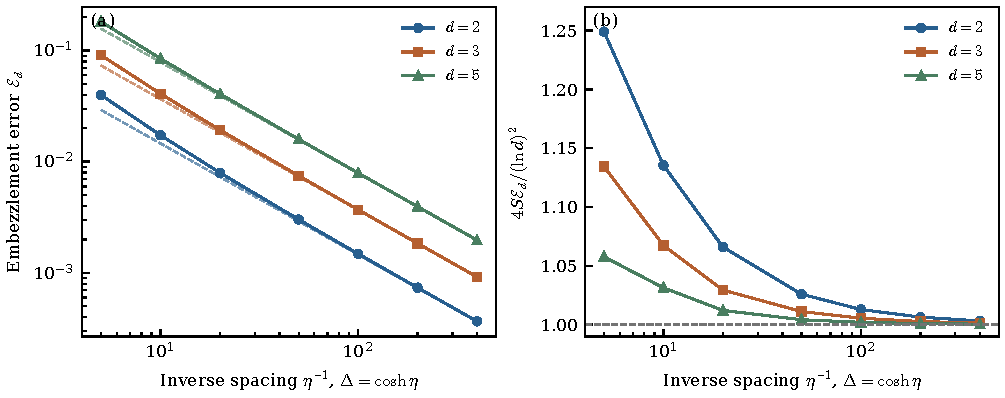
\includegraphics[width=\textwidth]{fig_xxz.pdf}
\caption{The XXZ corner-transfer-matrix spectrum in the symmetry-broken convention.
(a) The error for targets $d=2,3,5$, computed with exact integer
level multiplicities. Dashed curves show $3\eta(\ln d)^2/\pi^2$.
(b) The product $4S\mathcal E_d/(\ln d)^2$ approaches one.
Moving right sends $\eta=\operatorname{arcosh}\Delta$ to zero.
The omitted rank tail contributes less than $10^{-15}$ at each point.
The plotted values use floating-point evaluation.}
\label{fig:xxz}
\end{figure}

\begin{proposition}[Wick violation in the XXZ N\'eel phases]
\label{prop:xxz-nonquasifree}
For $1<\Delta\le21/20$, the Jordan--Wigner fermion state of each
boundary-selected N\'eel phase violates the gauge-invariant Wick identity
on two neighboring sites.
\end{proposition}

\begin{proof}
The two boundary limits of Ref.~\cite[Proposition~1.3]{ADW20} are
$U(1)$-invariant because the finite ground vectors have definite total
$Z$ spin. The staggered $Z$ rotation in their Eq.~(1.20) leaves $Z_j$
unchanged and conjugates translation to translation followed by a uniform
$Z$ rotation. Thus one-site translation still exchanges the two phases
in the convention of $H_\Delta$. Global spin flip exchanges the boundary
fields and hence the limiting states. It leaves the bond Hamiltonian
invariant and sends the even Jordan--Wigner hopping operator
$a_j^*a_{j+1}$ to its adjoint. Consequently the local $Z$ expectations
alternate between $m$ and $-m$, the bond energy $e_\Delta$ is independent
of the bond, and $|\omega(a_j^*a_{j+1})|=\alpha$ is also independent of
the bond.

Put $\eta=\operatorname{arcosh}\Delta$. In the finite-volume loop
representation of these same states~\cite[Theorem~4.2 and
Eqs.~(4.7)--(4.10)]{ADW20}, condition on the unoriented loops. The two
orientations of the loop through a site have probabilities
$e^{\pm\eta}/(e^\eta+e^{-\eta})$, with the signs exchanged for the
opposite boundary condition. Reversing that orientation flips the
site's Pauli $Z$ value. Thus the conditional mean has absolute value
$\tanh\eta$. Averaging and taking the boundary limits give
$m^2\le\tanh^2\eta=1-\Delta^{-2}$.

On an interval of $N$ sites, the fermionic covariance is a positive
contraction. A diagonal unitary makes all nearest off-diagonal
entries equal to $\alpha$. Its trace against the open-chain adjacency
matrix is then $2(N-1)\alpha$, at most the sum of the positive adjacency
eigenvalues. These are the positive members of
$2\cos(k\pi/(N+1))$, $1\le k\le N$. Dividing by $2(N-1)$ and taking
the limit gives $\alpha\le1/\pi$.

The bond energy equals the thermodynamic ground energy per site.
To see this, let $H_I$ be the open Hamiltonian of an interval $I$,
let $B_I$ be the two bonds crossing its boundary, and reset $I$ to
an open-chain ground vector. Summing the ground-state condition
$\omega(A^*[H_\Delta,A])\ge0$ over the reset channel's Kraus operators
gives $\omega(H_I)\le E_0(H_I)+2\|B_I\|$. The reverse bound is
variational. At $\Delta=1$ the exact Pauli-normalized energy is
$e_1=1-4\log2$~\cite{Hulthen38}. An $SU(2)$-averaged finite isotropic
ground state gives one third of its isotropic energy to each spin
component. Using it as a trial state for $H_\Delta$ and taking the
thermodynamic limit gives $e_\Delta\le e_1(\Delta+2)/3$.

The number relation $Z_j=2a_j^*a_j-1$ gives the Wick prediction
$\omega(Z_jZ_{j+1})=-m^2-4\alpha^2$. The hopping term has expectation
at least $-4\alpha$. The actual defect in the Wick identity therefore
satisfies
\begin{align*}
 \Delta\bigl(\omega(Z_jZ_{j+1})+m^2+4\alpha^2\bigr)
 &\le e_1(\Delta+2)/3+4/\pi+4\Delta/\pi^2+\Delta-\Delta^{-1}\\
 &\le \frac{61}{60}(1-4\log2)+\frac4\pi
       +\frac{21}{20}\left(\frac4{\pi^2}+\frac{41}{441}\right)<0.
\end{align*}
The first bound increases with $\Delta$ because $e_1>-3$. The last
strict inequality follows, for example, from $\log2>0.6931$ and
$\pi>3.1415$. The $U(1)$ symmetry sets the anomalous two-point
expectations to zero, so the defect excludes quasifreeness.
\end{proof}

\subsection{Critical bulk Hamiltonians obtained by local circuits}
\label{sec:bulk-circuits}

There is also an exact critical bulk construction at fixed coupling.
Write $h_j=(X_jX_{j+1}+Y_jY_{j+1})/2$. Controlled-phase gates turn
the XX interaction into density-dependent hopping throughout the chain.
Two choices distinguish preservation of the algebraic type from
preservation of the entire finite-chain Schmidt spectrum.

\begin{theorem}[Critical interacting bulk circuits]\label{thm:bulk-circuit}
The one-spin translation-invariant, finite-range interaction
\[
 H_{\mathrm{bulk}}=\sum_{j\in\mathbb Z}Z_{j-1}h_jZ_{j+2}
\]
has a pure gapless ground state whose physical half-chain factors are
type $\IIIone$ and satisfy Haag duality. The value of $G$ is one at
every vector in its ground-state sector. For its open finite-volume
circuit ground states, the Bell-pair embezzlement error tends to zero
and the game value tends to one.

The period-two bulk interaction
\[
 H_{\mathrm{pair}}=\sum_{j\in\mathbb Z}
 \bigl(h_{2j+1}+Z_{2j+1}h_{2j+2}Z_{2j+4}\bigr)
\]
has the same type and gaplessness properties. At the cut between $0$
and $1$, it has exactly the XX ground state's game value and
nonattainment property. On centred open intervals of $4m$ spins its
Schmidt spectrum equals that of the XX chain. Consequently every
finite-chain embezzlement law of Theorem~\ref{thm:xx-full-law} holds
unchanged for these interacting ground states.
\end{theorem}

\begin{proof}
Let $C_{j,j+1}=\operatorname{diag}(1,1,1,-1)$ on neighbouring spins.
Conjugation by this gate sends $X_j$ and $Y_j$ to $X_jZ_{j+1}$ and
$Y_jZ_{j+1}$, respectively, and fixes both $Z$ operators. The gate
commutes with $h_j$. The product over all bonds defines an involutive
automorphism $\alpha$: the gates commute and can be applied in two
layers of disjoint bonds. It commutes with one-site translation and
satisfies
\[
 \alpha(h_j)=Z_{j-1}h_jZ_{j+2}.
\]
The state $\omega_{\mathrm{XX}}\circ\alpha$ is a pure ground state
of the conjugate dynamics. Its GNS Hamiltonian is unitarily equivalent
to the XX GNS Hamiltonian and is therefore gapless.

At the cut, all gates except $C_{0,1}$ act separately in the two
halves. Thus $\alpha=\operatorname{Ad}(C_{0,1})\circ
(\alpha_L\otimes\alpha_R)$. Proposition~\ref{prop:factor} shows that
the represented half-chain pair is simultaneously unitarily conjugate
to the XX pair. Its type, Haag duality and sector-wide value one follow.
In a finite interval, conjugate the open XX Hamiltonian by the product
of its internal bond gates. The resulting Hamiltonian agrees with
$H_{\mathrm{bulk}}$ except for its boundary terms. Its ground state
converges locally to $\omega_{\mathrm{XX}}\circ\alpha$. Finite-support
approximations to the latter state's embezzling unitaries and game
measurements, as in the proof of Theorem~\ref{thm:value}, transfer both
limiting assertions to the finite intervals.

For $H_{\mathrm{pair}}$, apply the gates only on the pairs
$\{2j+1,2j+2\}$. They fix the hopping within each pair and dress the
interpair hopping by the two displayed $Z$ factors. No gate crosses
the indicated cut. The automorphism preserves both half-chain
algebras, and each finite-volume circuit is a tensor product of a
left and a right unitary. This preserves every Schmidt coefficient,
every state-specific game value, and whether its supremum is attained.
\end{proof}

These interactions contain genuine higher-order terms in the original
Jordan--Wigner fermions: the dressed hopping is multiplied by
$(1-2n_{j-1})(1-2n_{j+2})$, producing quartic and sextic terms.
Their exact circuit equivalence to XX explains why their critical
spectral laws can be transferred without approximation. The XXZ CTM
calculation supplies a different family of spectra to which the same
counting criterion applies.

\subsection{A quartic impurity in the XX representation}

Write $a(f)$ for the fermionic annihilator smeared with
$f\in\ell^2(\mathbb Z)$. Let $h$ be the single-particle nearest-neighbour
hopping operator $(h f)_j=f_{j-1}+f_{j+1}$, and let $\delta_j$ denote a
site basis vector. Put
\[
 f= h\delta_0/\sqrt2,\qquad g=h\delta_1/\sqrt2,\qquad
 V=a^*(f)a(f)a^*(g)a(g).
\]
The two vectors are orthonormal. Thus $V$ is a self-adjoint projection.
It is even and its Jordan--Wigner image $V_{\rm s}$ is a spin operator
supported on $[-1,2]$. Let $H_\lambda$ denote the spin XX interaction
perturbed by $\lambda V_{\rm s}$, where $\lambda\in\mathbb R$.

\begin{theorem}[A pure ground state in the XX sector]\label{thm:impurity}
For $0<|\lambda|<1/\sqrt8$, $H_\lambda$ has a pure ground state in the
unperturbed XX GNS representation, distinct from the original ground state.
Its two physical half-chains are type $\III$ factors in Haag duality. The
ground-state GNS Hamiltonian has positive spectrum accumulating at zero.
In particular the value of the game $G$ is one in this ground state
and at every vector in its sector, by Theorem~\ref{thm:value} and its sector-wide proof.
\end{theorem}

\begin{corollary}[A ground state that violates the quasifree description]\label{cor:nongaussian}
For $0<|\lambda|<\bigl(\frac12-\frac{4}{3\pi}\bigr)^2/(4\sqrt8)$, the ground state in
Theorem~\ref{thm:impurity} can be chosen gauge invariant with a pure,
nonquasifree Jordan--Wigner fermionic state.
\end{corollary}

\begin{corollary}[Finite impurity chains]\label{cor:impurity-finite}
Under the coupling hypothesis of Theorem~\ref{thm:impurity}, every local
subsequential limit of the centred even-length open-chain ground states is
a pure ground state in the XX sector. Their finite-chain game value tends
to one for the game $G$. Their Bell-pair embezzlement error also tends to zero.
\end{corollary}

The choice $f=h\delta_0/\sqrt2$, $g=h\delta_1/\sqrt2$ suppresses the
interaction at the Fermi points. A pull-through estimate bounds the expected
number of particle--hole excitations by $8\lambda^2$, uniformly in the
volume. This retains a nonzero overlap with the free vacuum and places an
infinite ground state in the same irreducible representation. Compactness
of the excitation vectors gives the finite-chain conclusion. The
four-excitation component of the quartic interaction then excludes a
quasifree description at small nonzero coupling. Full proofs are in
Appendix~\ref{app:interacting}.



\section{Quantum fields}\label{sec:qft}

\begin{corollary}[Vacuum of a free field]\label{cor:qft}
Let $\Omega$ be the vacuum of the free scalar field of mass $m>0$ in $d+1$ space-time
dimensions, with $d\ge1$. If Alice and Bob measure in complementary wedges, then
$\omega(\Omega)=1$ and every strategy loses with positive probability. For any split pair
$M_A\subseteq\mathcal N\subseteq M_B'$ with $\mathcal N$ a type I factor, the loss of every
strategy is at least $\cE(\rho_{\mathcal N})/C>0$, where $\cE(\rho_{\mathcal N})$ is the
Bell-pair error~\eqref{eq:Ed} evaluated on the eigenvalues of the vacuum density matrix on
$\mathcal N$.
\end{corollary}

\begin{proof}
The vacuum is cyclic and separating for the wedge algebra by the Reeh--Schlieder property
and locality~\cite{Haag}. The Bisognano--Wichmann theorem identifies complementary wedge
algebras as commutants and the vacuum modular group with the Lorentz
boosts~\cite{BisognanoWichmann75}. The wedge algebra is a factor of type
$\IIIone$~\cite{Driessler75,Haag}. Van Luijk, Stottmeister, Werner and Wilming proved
bipartite embezzlement for the wedge vacuum~\cite[Theorem~97]{vLSWW24} and reported it in
Ref.~\cite{vLSWWPRL24}. The ancilla argument in the proof of Theorem~\ref{thm:value} gives
value one for $G$.

For the free massive scalar field, write a point of the positive mass shell as
\[
 p^0=m_\perp\cosh\theta,\qquad p^1=m_\perp\sinh\theta,
 \qquad m_\perp=\sqrt{m^2+|p_\perp|^2}.
\]
Then $d^dp/(2p^0)=\tfrac12\,d\theta\,d^{d-1}p_\perp$, and a boost in the wedge direction
translates the rapidity $\theta$. Fourier transformation in $\theta$ identifies the
one-particle boost generator with multiplication by a real coordinate on a space with
Lebesgue measure, so its vector spectral measures have no atoms. On each positive-particle
sector of symmetric Fock space the generator is the restriction of a sum of one-particle
generators. Product vectors have convolution spectral measures, which are atomless, and
are total in the unsymmetrized tensor power. The spectral projections onto singletons
therefore vanish on each positive-particle sector. Only the vacuum line contributes a
modular eigenvector. The Bisognano--Wichmann identification of the vacuum modular group
with the boosts thus excludes $2$ from the point spectrum of the modular operator.
Proposition~\ref{prop:modular-obstruction} rules out perfect play.

For a split pair, $\cH=\cH_1\otimes\cH_2$ with $\mathcal{N}=\mathcal{B}(\cH_1)\otimes1$.
Every strategy is a tensor-product strategy on the pure state $\Omega$, whose Schmidt
probabilities are the eigenvalues of $\rho_{\mathcal N}$. Theorem~\ref{thm:equiv}
together with~\eqref{eq:range} gives the bound. For example, for double cones
$\mathcal O_1,\mathcal O_2$ with $\overline{\mathcal O_1}\subset\mathcal O_2$, the split
property supplies the required factor for $\mathcal M(\mathcal O_1)$ and
$\mathcal M(\mathcal O_2')$~\cite{Buchholz74,DoplicherLongo84}.
\end{proof}

Summers and Werner showed that the vacuum violates the Bell--CHSH inequality maximally for
complementary wedges~\cite{SummersWerner87c,SummersWerner87b}. The first statement of
Corollary~\ref{cor:qft} is the corresponding result for a game that no system of type I or II
can win.


\section{What the game reads}\label{sec:discussion}

The game tests approximate invariance under adding a Bell pair, hence the
ratio two in the spectrum. This is a state-specific test. For a factor and its full commutant, so that Haag duality holds, the
classification uses the stronger statement that the value is one at
\emph{every faithful normal state}. Under the flow criterion of
Ref.~\cite[Section~4]{TG}, that statement is equivalent to
$1/2\in S(M_A)$: it holds for III$_1$ and also for
III$_\lambda$ with $\lambda=2^{-1/k}$ for a positive integer $k$.
A single fixed state with a very high score does not establish this
all-states property.

Using the ratio-three game and its corresponding factor criterion from Ref.~\cite{TG}, we can combine that game with $G$ by sending
both players a common tag telling them which test is being played.
With equal tag probabilities the resulting value is exactly
$(\omega_2+\omega_3)/2$, because strategies on the two tagged question
sets can be chosen independently. Value one at every faithful normal state
then requires both $1/2$ and $1/3$ in the factor invariant and singles out
III$_1$. The incommensurate-ratio mechanism is already part of the
flow-of-weights account of embezzlement~\cite{vLSWW24}; the tagged game is
an operational way of combining the tests.

Finite tensor powers show the same selectivity. For pairs with Schmidt
probabilities $(2/3,1/3)$, the Bell-pair error decreases, whereas ratios
three and four retain a positive defect (Table~\ref{tab:pairs}). Extensive
entropy is compatible with either behavior.

The positive floors follow directly from the multiplicative spacing.
If the nonzero probabilities lie in $c\,r^{\mathbb Z}$ with $r>2$, put
$a=1/\sqrt2$, $b=\sqrt{r/2}$ and
$t_m=(D\lambda)_m/\lambda_m$ wherever $\lambda_m>0$.
Each $t_m$ lies outside $(a,b)$, so
$(a+b)t_m\le t_m^2+ab$. Multiply by $\lambda_m^2$ and sum;
since $\sum_{\lambda_m>0}\lambda_m^2t_m^2\le1$, this gives
\[
\cE\ge2-2\frac{1+ab}{a+b}>0.
\]
For ratios three and four the bounds are respectively
$2-(1+\sqrt3)/\sqrt2=0.0681483\ldots$ and
$2-4\sqrt2/3=0.1143819\ldots$, uniformly in the number of copies.

\begin{table}[htb]
\centering\small
\begin{tabular}{@{}lcccccc@{}}
\toprule
Schmidt probabilities & Ratio & $n=1$ & $16$ & $64$ & $256$ & $1000$\\
\midrule
$(2/3,1/3)$ & 2 & 0.3905 & 0.1392 & 0.0417 & 0.0179 & 0.0091 \\
$(3/4,1/4)$ & 3 & 0.3270 & 0.1079 & 0.0718 & 0.0682 & 0.0681 \\
$(4/5,1/5)$ & 4 & 0.3029 & 0.1286 & 0.1146 & 0.1144 & 0.1144 \\
\bottomrule
\end{tabular}
\caption{Bell-pair embezzlement error for $n$ copies of the indicated
two-qubit state, computed with exact binomial multiplicities.}\label{tab:pairs}
\end{table}

The explicit strategy also clarifies the experimental requirements. In a
known Schmidt basis, the measurements reduce to reversible quotient and
remainder arithmetic followed by one fixed five-level measurement.
Their dependence on Schmidt rank is polynomial in its logarithm. Learning
or implementing that basis for a many-body state is a separate task;
entanglement-Hamiltonian spectroscopy and tomography address aspects of
it~\cite{Dalmonte18,Kokail21}. The finite sine-profile resource avoids
this step by choosing the computational basis from the outset.
Its separation from all flat-spectrum resources is quantitative and
survives the preparation error stated in Section~\ref{sec:operational-lower}.

The spectral counting criterion determines the sharp extraction cost and
its growing-target crossover. The original game has an assisted
certificate at $N=2^{19}$ with one shared $\Phi_9$, and a chain-only
certificate at $N=2^{84}$. The four-spin witness comes from tilted CHSH,
with classical play in the original game branch. The half-chain type
guarantees value one throughout the critical XX sector, and the modular
spectrum obstructs attainment at the ground state. The XXZ law concerns
the corner-transfer-matrix spectrum as the anisotropy approaches one
from above, with the physical spectral identification taken as input.
The cut-preserving bulk circuit retains
the finite critical XX Schmidt spectrum by exact conjugacy.

\section*{How this work was done}
The authors chose the questions and directed the work, which used AI
models from two developers: Claude Fable~5.2 (Anthropic) and GPT-6
Astra and GPT-6.1 Sol (OpenAI). Before release the manuscript was
checked refutation-first by fresh model instances that had not worked
on it: an earlier revision in three independent passes by Claude
Opus~5.5, two on the proofs and one on priority and credit, and the
following revision by GPT-6.1 Sol, which also reran the chain-only
certificate. This version applies the wording fixes from that check,
made with Claude Opus~5.5. The game constants, loss bounds and
separations rest on exact or outward-rounded certificates that the
accompanying archive re-checks; the other numerical values are
floating-point computations with the error control of
Appendix~\ref{app:numerics}. The theorems are proved in the text; none
is formalized in a proof assistant. The authors take responsibility for
every claim.

\section*{Reproducibility}
The accompanying source archive contains the numerical data, exact game certificates, and programs used to reproduce the calculations and figures. The game quadratic form is evaluated from all 243 question pairs, with its matrix identity checked in $\mathbb Q(\sqrt2)$. Numerical methods and truncation estimates are given in Appendix~\ref{app:numerics}.


\appendix

\section{The game}\label{app:game}

We reproduce the definition of Ref.~\cite[Section~2.1]{TG}; the complete rule table is in the
ancillary files of that paper.

\paragraph{The flagged magic-square game $G_{\mathrm{FMS}}$~\cite{Mancinska26}.} Let
$\mathsf{R}=\{{+}{+}{+},{+}{-}{-},{-}{+}{-},{-}{-}{+}\}$ be the sign triples of product $+1$, and
$\mathsf{C}_j$ the sign triples of product $\eta_j$, where $\eta=(+,+,-)$. Fix
$r_0=c_0={+}{+}{+}$ and $r_1=c_1={+}{-}{-}$. Alice's questions are $R_1,R_2,R_3,T_0,T_1$ and
Bob's are $C_1,C_2,C_3,U_0,U_1$. To a row question $R_i$ Alice answers a triple in
$\mathsf{R}$ or the flag $f$; to a column question $C_j$ Bob answers a triple in $\mathsf{C}_j$
or $f$. To $T_x$ Alice answers a triple in $\mathsf{C}_1\setminus\{c_x\}$ or a sign; to $U_y$
Bob answers a triple in $\mathsf{R}\setminus\{r_y\}$ or a sign.

The rules are as follows. At a pair $(R_i,C_j)$, two flags win and a single flag loses; if
neither player flags, Alice's sign for column $j$ must equal Bob's sign for row $i$, as in the
magic-square game. At $(T_x,C_1)$, Alice must answer a sign exactly when Bob's answer is $f$ or
$c_x$, and if she answers a triple, Bob must answer the same triple. The pair $(R_1,U_y)$ has
the same rule with the roles exchanged and $r_y$ in place of $c_x$. At $(T_x,U_y)$, two signs
$s$ and $s'$ must satisfy $ss'=(-1)^{xy}$, and every other pair of answers wins. All remaining
question pairs are won with any answers. The 25 question pairs are asked with equal probability. The ideal strategy uses the state
$\bigl(\ket{ff}+\sqrt2\sum_{i=1}^4\ket{ii}\bigr)/3$ on $\C^5\otimes\C^5$, a flag level and two
qubits per player, with the magic-square measurements on the qubits; the factor $\sqrt2$ is the
ratio tested by the questions $T_x$ and $U_y$.

\paragraph{The game $\GIII$.} Take nine copies of $G_{\mathrm{FMS}}$, indexed by $j\in\Z/9\Z$,
and one further question $\mathrm{Lab}$ for Bob with answers $\ell\in\Z/9\Z$. Besides the
$9\times25$ pairs inside the copies there are $18$ pairs
\begin{align*}
(R_1^{\,j},\mathrm{Lab})&:\quad\text{win iff }\bigl[\text{Alice answers } f\bigr]\Leftrightarrow\bigl[\ell=j\bigr],\\
(R_2^{\,j},\mathrm{Lab})&:\quad\text{win iff }\bigl[\text{Alice answers } {+}{+}{+}\bigr]\Leftrightarrow\bigl[\ell\in\{j+1,j+2\}\bigr].
\end{align*}
The 243 pairs are asked with equal probability. The first family makes the nine flags a
partition of unity, each matched with a label of Bob. The second identifies one of the four
two-qubit levels of copy $j$ with the flags of copies $j+1$ and $j+2$. Together with the ratio
$\sqrt2$ this yields~\eqref{eq:bridge}.


The explicit measurements and their loss for general Schmidt spectra are given in Section~\ref{sec:operational-strategy}.


\section{The explicit robustness constant}\label{sec:explicit-robust}

The lower comparison of Ref.~\cite{TG} uses a flagged-sector estimate from
Ref.~\cite{PP}. We obtain explicit constants for the sector estimate and
the nine-copy comparison. Write $\operatorname{Sch}(v)$ for the decreasing
Schmidt-amplitude list of an arbitrary vector $v$, padded by zeroes. Write
$k\times s$ for $k$ copies of a list $s$, arranged in decreasing order.
We use
\begin{equation}\label{eq:sch-contract-explicit}
 \|\operatorname{Sch}(v)-\operatorname{Sch}(w)\|_2\le\|v-w\|.
\end{equation}
This follows by applying von Neumann's trace inequality to the
Hilbert--Schmidt coefficient operators of the two vectors and expanding
both squares. Finite-rank approximation gives the same inequality in
arbitrary Hilbert spaces.

\begin{lemma}[Quantitative flagged-sector estimate]\label{lem:explicit-sector}
Let $\psi$ be a vector and the measurements of one flagged magic-square
copy be projective. Let $F$ be Alice's $R_1$ flag projection and let $N$
be the sum of the forbidden masses on the 25 internal pairs, evaluated
on $\psi$. Then
\begin{equation}\label{eq:explicit-sector}
 \|\operatorname{Sch}((I-F)\psi)
      -4\times(\sqrt2\,\operatorname{Sch}(F\psi))\|_2\le 210\sqrt N .
\end{equation}
\end{lemma}

\begin{proof}
We omit tensor identities for local operators. Denote Alice's row flag
projections by $F_i$, and Bob's column flag projections by $G_j$. Put
$F=F_1$, $G_\star=G_1$, and $\mu=(I-F)(I-G_\star)\psi$. For the row--column
pair $(i,j)$ let $u_{ij}^2$ be its forbidden mass and let
$M=\sum_{ij}u_{ij}^2$. Define
\[
 d_A=\|F(I-G_\star)\psi\|,\qquad
 d_B=\|(I-F)G_\star\psi\|,\qquad d^2=d_A^2+d_B^2\le u_{11}^2.
\]
The last inequality and $\|(F_i-G_j)\psi\|\le u_{ij}$ use the flag-mismatch
rule.

\paragraph{Extracting the magic-square state.}
For each cell let $A_{ij},B_{ij}$ be the two local sign observables, giving
every flag the sign $+1$. They are self-adjoint unitaries and satisfy
$\|(A_{ij}-B_{ij})\psi\|\le\beta_{ij}$, where $\beta_{ij}=2u_{ij}$.
Alice's rows and Bob's columns commute within each context. Alice's row
products and Bob's first two column products are $I$, and
\[
 B_{33}=-B_{13}B_{23}+2G_3.
\]
Denote the generators at cells $(11,12,21,22)$ by $(a,b,c,d_0)$ on Alice
and by the same primed symbols on Bob. A word of $k$ local observables on
$\psi$ differs from the reversed word on the other party by at most the
sum of the $k$ cell bounds $\beta_{ij}$. To see this, replace the
rightmost factor on $\psi$ and commute it to the left of the remaining
factors. In particular, a difference $L$ of two signed local words,
followed by a one-letter suffix $s$, has
$\|Ls\psi\|\le\|L\psi\|+2\beta_s$.

Write $W=\sum_{ij}\beta_{ij}$, and let $[q,r]=qr-rq$ and
$\{q,r\}=qr+rq$. On either party the three expressions
\[
 d_0\{b,c\}a,\qquad b\{a,d_0\}c,\qquad c\{a,d_0\}b
\]
applied to $\psi$ differ from $2G_3\psi$ by at most $W$.
In each expression the two terms are a product of column pairs and a
product of row pairs. The column pairs are the cells $31,32$ on Bob,
and their product transfers to Alice's $A_{33}$. The row pairs are the
cells $13,23$ on Alice, and their product transfers to Bob's
$B_{13}B_{23}$. The remaining transfer is the cell $33$.
Expanding each product on the other party by the reversed-word rule
costs in total each of the nine bounds $\beta_{ij}$ once. Reversing the
order of the two row or column pairs is allowed at the transfer, by
commutation in Bob's column 3 or Alice's row 3. Also, if two generators
$q,r$ commute on the other party, then
$\|[q,r]\psi\|\le2(\beta_q+\beta_r)$ by two word transfers.

We use the real two-qubit Pauli group $\mathcal P$ generated by
$a=ZI$, $b=IZ$, $c=IX$, $d_0=XI$ and $J=-I$, with the usual Pauli
matrices $Z,X$. Its 32 elements have unique signed normal words in any
fixed ordering of $a,b,c,d_0$, with each generator appearing at most once.
The anticommuting pairs are $(a,d_0)$ and $(b,c)$, and the other pairs
commute. For $g\in\mathcal P$, let $A_g$ evaluate its signed normal word
in the physical observables, using the order $(c,d_0,a,b)$. Define
$B_g$ on Bob using $(b,d_0,a,c)$. The local isometries
\[
 V_A v=32^{-1/2}\sum_{g\in\mathcal P}|g\rangle A_g v,\qquad
 V_B v=32^{-1/2}\sum_{g\in\mathcal P}|g\rangle B_g v
\]
have their registers in the $-1$ eigenspace of $\rho(J)$, where
$\rho(h)|g\rangle=|gh^{-1}\rangle$ is the right regular action.
The exact commutation of the last two generators in each order gives
$V_A a=\rho(a)V_A$, $V_A b=\rho(b)V_A$, and
$V_B a'=\rho(a)V_B$, $V_B c'=\rho(c)V_B$ on the full input spaces.

For a generator $h$ write $\alpha_{Ah}=\|(V_A A_h-\rho(h)V_A)\mu\|$,
and define $\alpha_{Bh}$ in the same way. These norms are the
root-mean-square errors of rewriting the physical word for $g$
followed by $h$ into the word for $gh$. Put
\[
 L_A=W+2u_{13}+2d_A,\qquad L_B=W+2u_{13}.
\]
The table gives the rewriting bounds on $(I-G_\star)\psi$ for Alice and
$(I-F)\psi$ for Bob. The three columns cover presence of only the
first, only the second, and both of the last two letters in the word
for $g$. With neither letter present the rewriting is exact.
\[
\begin{array}{c|ccc}
 &\text{first}&\text{second}&\text{both}\\ \hline
 A,c
 &2(\beta_a+\beta_c)& L_A+2\beta_a
 & L_A+2\beta_a+2(\beta_a+\beta_c+\beta_b)\\
 A,d_0
 &L_A+2\beta_c&2(\beta_b+\beta_{d_0})
 &L_A+2(\beta_b+\beta_{d_0})\\
 B,b
 &2(\beta_a+\beta_b)&L_B+2\beta_a
 &L_B+2\beta_a+2(\beta_a+\beta_b+\beta_c)\\
 B,d_0
 &L_B+2\beta_b&2(\beta_c+\beta_{d_0})
 &L_B+2(\beta_c+\beta_{d_0})
\end{array}
\]
For the anticommutator swaps the flag correction costs at most
$2\|(I-G_\star)G_3\psi\|\le2u_{13}+2d_A$ on Alice and
$2\|(I-F)G_3\psi\|\le2u_{13}$ on Bob. When the swap has no suffix,
transfer the trailing letter of the displayed anticommutator identity
to the other party before projecting. Use $a$ for the pair $(b,c)$, $c$
on Alice for $(a,d_0)$, and $b$ on Bob for $(a,d_0)$. The transferred
letter commutes with the opposite flag $G_\star$ or $F$. When the
$(a,d_0)$ swap already has a suffix, use the identity with that suffix
and project directly. In the remaining swaps only the commutator
bound and, if present, one suffix transfer are needed.

On $\mu$ add $2d_A$ or $2d_B$ to each nonzero case in the table, because
the difference of the two signed words has norm at most two. Each case
has register weight $1/4$. Write
$v=(u_{11},u_{12},\ldots,u_{33},d_A,d_B)^{\mathsf T}$ in row-major
order, and let $L_{Ah}$ and $L_{Bh}$ be the coefficient matrices of
the three bounds for each row of the table, including the additions
$2d_A$ or $2d_B$. Thus $\alpha_{Ah}\le\|L_{Ah}v\|_2/2$ and
likewise for Bob.

The consistency errors $\delta_h=\|(A_h-B_h)\mu\|$ satisfy
\[
 \delta_a\le 2u_{11},\quad
 \delta_b\le 2u_{12}+2d_B,\quad
 \delta_c\le 2u_{21}+2d_A,\quad
 \delta_{d_0}\le 2u_{22}+u_{12}+u_{21}+d_A+d_B .
\]
For $a,b,c$, use commutation with the corresponding anchor flags.
For $d_0$, the cell difference commutes with $G_2$ and with $F_2$.
Compare $\mu$ to $(I-G_2)\psi$ or $(I-F_2)\psi$, at distances at most
$d_B+u_{12}$ and $d_A+u_{21}$, respectively, and average the two bounds.
Write $\ell_h(v)$ for the corresponding linear upper bound on $\delta_h$.

The $-1$ register sector carries $ZI,IZ,IX,XI$ on two qubits and an
identity on a multiplicity space. Indeed the four joint eigenspaces of
$\rho(a),\rho(b)$ are identified with the joint $+1$ eigenspace by
$\rho(d_0),\rho(c)$, which flip their respective signs and commute.
Let $w=(V_A\otimes V_B)\mu$. The four simultaneous involutions
$K_h=\rho_A(h)\rho_B(h)$ commute and their joint $+1$ projection
$\Pi$ has range $\Phi_4\otimes\mathcal K_A\otimes\mathcal K_B$.
The generators $ZI,IZ$ first enforce equal bits on both registers and
$IX,XI$ then enforce equal coefficients on the four equal-bit basis
vectors. Put $w_0=\Pi w=\Phi_4\otimes j$ and $\eta=\|w-w_0\|$. Since
$\|(I-K_h)w\|\le\alpha_{Ah}+\delta_h+\alpha_{Bh}$,
\[
 4\eta^2\le\sum_h(\alpha_{Ah}+\delta_h+\alpha_{Bh})^2\le v^{\mathsf T}Hv .
\]
The first inequality follows from $I-\Pi\le\sum_h(I-K_h)/2$.
For the second, use weighted Cauchy--Schwarz with weights $(1,6)$
for $b$, $(1,5)$ for $c$, and $(2,6,5)$ for $d_0$. In terms of the
linear forms above the resulting matrix is given by
\begin{align*}
 v^{\mathsf T}Hv
 &=\ell_a(v)^2+7\ell_b(v)^2+6\ell_c(v)^2+\tfrac{13}{2}\ell_{d_0}(v)^2\\
 &\quad+\tfrac7{24}\|L_{Bb}v\|_2^2+\tfrac3{10}\|L_{Ac}v\|_2^2
   +\tfrac{13}{24}\|L_{Ad_0}v\|_2^2+\tfrac{13}{20}\|L_{Bd_0}v\|_2^2.
\end{align*}
All its entries are nonnegative. For
\[
 D_*=\operatorname{diag}(.561,1,1,1,1,1,1,1,1,.439,.439),\qquad
 q=(1000,623,452,634,517,226,226,226,226,833,553)^{\mathsf T},
\]
the integers $\lceil1000(Hq)_i/(D_*q)_i\rceil$ in order are
\[
 (521543,521579,521308,521552,521430,521308,521308,521308,521308,521546,521180).
\]
Thus $Hq\le521.6D_*q$. Using
$2v_iv_j\le v_i^2q_j/q_i+v_j^2q_i/q_j$ entrywise gives
$v^{\mathsf T}Hv\le521.6v^{\mathsf T}D_*v\le521.6M$, the last
inequality by $d_A^2+d_B^2\le u_{11}^2$. This gives
$\eta\le11.42\sqrt M$.

\paragraph{Comparing the flag and magic-square sectors.}
Embed each local space into a direct sum of a flag space and an
extracted magic-square space, by $v\mapsto Fv\oplus V_A(I-F)v$ for Alice
and $v\mapsto G_\star v\oplus V_B(I-G_\star)v$ for Bob. Let $P,Q$ be the two
flag-space projections and let $\Psi$ be the embedded state. Write
$\varphi=PQ\Psi$, $\zeta=\varphi+w_0$, and $e=\Psi-\zeta$. The components
of $e$ in $P(I-Q)$, $(I-P)Q$ and $(I-P)(I-Q)$ have norms
$d_A,d_B,\eta$, respectively. The measurements transport to the images
of the isometries and can be extended as projective measurements by
assigning the orthogonal complement to one outcome.

On either magic register let $R_y$ be the projection onto
$r_y=|0\rangle|y\rangle$ and $C_x$ the projection onto
$c_x=|0\rangle(|0\rangle+(-1)^x|1\rangle)/\sqrt2$, tensored with the
identity on its multiplicity and original local space. Extend these
projections by zero on the flag spaces and use superscripts $A,B$
for the party. The exact intertwining for Alice's $a,b$ and Bob's
$a',c'$ means that $P_y=P+R_y^A$ and $Q_x=Q+C_x^B$ act on $\Psi$
as the calibrated physical coarse-grainings $f\ \text{or}\ r_y$
and $f\ \text{or}\ c_x$. Put $E_x^0=P+C_x^A$ and $H_y^0=Q+R_y^B$.
These satisfy $E_x^0\zeta=Q_x\zeta$ and $H_y^0\zeta=P_y\zeta$.

Let $E_x,H_y$ be the actual sign projections of $T_x,U_y$, and let
$t_x,u_y'$ be the forbidden masses at $(T_x,C_1)$ and $(R_1,U_y)$.
The mismatch rule gives
$\|(E_x-Q_x)\Psi\|\le\sqrt{t_x}$ and
$\|(H_y-P_y)\Psi\|\le\sqrt{u_y'}$. Set $T=\sum_x t_x+\sum_y u_y'$.
Define $\xi_{xy}=E_x^0H_y^0\zeta$. Using the two exact relations on
$\zeta$ gives
\begin{align*}
 E_xH_y\Psi-\xi_{xy}
 &=H_y(E_x-Q_x)\Psi+E_x^0(H_y-P_y)\Psi\\
 &\quad+H_y(Q_x-E_x^0)e+E_x^0P_y e .
\end{align*}
The first two terms together have norm at most $2\sqrt T$ in the
direct sum over $x,y$. For the third, each difference of projections
has operator norm at most one, so the direct-sum norm is at most
$2\sqrt{d^2+\eta^2}$. For the fourth, $E_x^0P_y$ is the identity on
Alice's flag and equals $C_x^A R_y^A$ on her magic space, with
$\sum_{xy}R_y^A C_x^A R_y^A\le I$. Hence
\begin{equation}\label{eq:explicit-sign-support}
 \left(\sum_{xy}\|E_xH_y\Psi-\xi_{xy}\|^2\right)^{1/2}
 \le 2\sqrt T+2\sqrt{d^2+\eta^2}+\sqrt{\eta^2+4d_A^2+d_B^2}.
\end{equation}

Let $U_x,V_y$ be the local sign unitaries, acting by the measured sign
on the sign subspace and by $+1$ on its complement. Put
$t_{xy}=(-1)^{xy}$ and let $S$ sum the forbidden masses on the four
sign pairs. Then
\[
 \sum_{xy}\|(U_x-t_{xy}V_y)E_xH_y\Psi\|^2=4S.
\]
The ideal support vector is $\xi_{xy}=\varphi+\chi_{xy}$ with
$\chi_{xy}=t_{xy}|c_xr_y\rangle h$ and $h=j/(2\sqrt2)$, by the
overlap of the two selected magic-register vectors. Define
$b_{xy}=(U_x-t_{xy}V_y)\xi_{xy}$ and $B^2=\sum_{xy}\|b_{xy}\|^2$.
Equation~\eqref{eq:explicit-sign-support} gives
\[
 B\le 2\sqrt S+4\sqrt T+4\sqrt{d^2+\eta^2}
                 +2\sqrt{\eta^2+4d_A^2+d_B^2}.
\]

To compare $\varphi$ and $h$, project the four $b_{xy}$ onto $PQ$.
The resulting differences are $P U_x\varphi-t_{xy}Q V_y\varphi$.
For four vectors $v_x,w_y$ in a common space,
$2w_0=(w_0-v_0)+(v_0-w_1)+(w_1+v_1)+(w_0-v_1)$.
Cauchy--Schwarz therefore bounds $\|w_0\|^2$ by the sum of the four
squared differences $\|v_x-t_{xy}w_y\|^2$, and the same holds for
$v_0$. In particular,
$\|Q V_0\varphi\|^2\le\sum_{xy}\|PQ b_{xy}\|^2$.
Next project onto $C_x^A R_y^B$ and remove the explicit qubit factors
and the scalar sign $t_{xy}$. The four differences now involve the
compressions of $U_x$ to $c_x$ and of $V_y$ to $r_y$, acting on the
common vector $h$. This gives
$\|C_0^A U_0\chi_{00}\|^2\le\sum_{xy}\|C_x^A R_y^B b_{xy}\|^2$.

The components of $U_0\chi_{00}-V_0\varphi$ in $PQ$ and $C_0^A$
have exactly these two bounded norms. Its remaining components, in
$P(I-Q)$ and $I-P-C_0^A$, are
$P(I-Q)b_{00}$ and $(I-P-C_0^A)R_0^B b_{00}$, respectively.
These are orthogonal to one another and to the two projections
of $b_{00}$ used in the cycle bounds. Adding the squared norms yields
$\|U_0\chi_{00}-V_0\varphi\|\le B$.
By~\eqref{eq:sch-contract-explicit} and local unitarity,
$\|\operatorname{Sch}(h)-\operatorname{Sch}(\varphi)\|_2\le B$.

The list of $w_0$ is $4\times(\sqrt2\,\operatorname{Sch}(h))$.
The extracted $F\psi$ is within $d_A$ of $\varphi$, and the extracted
$(I-F)\psi$ is within $\sqrt{d_B^2+\eta^2}$ of $w_0$. The left side of
~\eqref{eq:explicit-sector} is therefore bounded by
\[
 \sqrt{d_B^2+\eta^2}+2\sqrt2\,d_A+2\sqrt2\,B
 \le 209.6\sqrt M+8\sqrt2\sqrt T+4\sqrt2\sqrt S .
\]
For the numerical bound use
$\sqrt{1+11.42^2}<11.464$, $\sqrt{4+11.42^2}<11.594$ and
$2\sqrt2<2.828428$. Since $209.6^2+160<210^2$ and $M+T+S=N$,
Cauchy--Schwarz proves~\eqref{eq:explicit-sector}.
\end{proof}

\begin{proof}[Lower bound in Theorem~\ref{thm:equiv}]
First make the measurements projective by local isometries. For a
finite POVM $(M_a)_a$ on $\mathcal H$, its isometry
$Wv=\sum_a\sqrt{M_a}v\otimes|a\rangle$ maps into an outcome register
space $\mathcal H\otimes\mathbb C^m$. A common enlarged space is
$\mathcal H\oplus(\mathcal H\otimes\mathbb C^m)$, with the input in the
first summand and $m$ at least the largest number of outcomes. For
each question the self-adjoint unitary
$(v,w)\mapsto(W^*w,Wv+(I-WW^*)w)$ exchanges the input with the range
of $W$. Conjugating the outcome-coordinate projections, with the
first summand and any unused coordinates assigned to a fixed
outcome, gives the required projective measurement. This dilation
preserves correlations and the nonzero Schmidt amplitudes.

Write $\Lambda=\operatorname{Sch}(\psi)$, $Q_j$ for Bob's label
projections, and $F_j$ for the nine $R_1$ flags on Alice. Let
$d_j=\|(F_j-Q_j)\psi\|$, $N_L=\sum_j d_j^2$, and $N_F=\sum_j N_j$,
where $N_j$ is the internal forbidden mass of copy $j$. For the
strategy's losing probability $\varepsilon$ the disjoint budgets
give $N_F+N_L\le243\varepsilon$.

To separate the label sectors, use the local column operator
$Tv=\sum_j F_jv\otimes|j\rangle$ on Alice, with
$A=T^*T=\sum_jF_j$. Add an unused register entry and extend the partial
isometry in the polar decomposition $T=V A^{1/2}$ to an isometry
$V$ by mapping $\ker A$ into that entry. Since $A\ge F_j$, operator
monotonicity of the square root gives $A^{1/2}\ge F_j$. On the
orthogonal Bob labels this yields $A^{1/2}\ge\sum_j F_jQ_j$, and
\[
 \|(V-T)\psi\|^2=\|(I-A^{1/2})\psi\|^2
 \le \langle\psi,(A+I-2\textstyle\sum_j F_jQ_j)\psi\rangle=N_L.
\]
Apply the exact label isometry on Bob. For any label subset $I_0$,
the raw map $T$ on $\sum_{j\in I_0}Q_j\psi$ then differs from
$\sum_{j\in I_0}Q_j\psi\otimes|j,j\rangle$ by a vector of squared
norm $\sum_{j\in I_0,k}\|Q_j(F_k-Q_k)\psi\|^2\le N_L$.
The same input restricted to $I_0$ can only decrease the
$(V-T)$ error. Thus the two local isometries give a vector within
$2\sqrt{N_L}$ of the target.
Let $S_j=\operatorname{Sch}(Q_j\psi)$ and let $\bigsqcup$ denote
sorted union. The target is orthogonal on both sides, so
\[
 \left\|\operatorname{Sch}\left(\sum_{j\in I_0}Q_j\psi\right)
      -\bigsqcup_{j\in I_0}S_j\right\|_2\le2\sqrt{N_L}.
\]

Use this estimate on each complementary label set and replace $F_j$
by $Q_j$ in~\eqref{eq:explicit-sector} using
~\eqref{eq:sch-contract-explicit}. Then
\[
 \left\|\bigsqcup_{k\ne j}S_k-4\times(\sqrt2 S_j)\right\|_2
 \le 210\sqrt{N_j}+(1+2\sqrt2)d_j+2\sqrt{N_L}.
\]
Write $U=\bigsqcup_j S_j$ and
$\Delta(s)=\|2\times s-\sqrt2\,s\|_2$. Concatenate the nine list
comparisons and sort each side. Sorting cannot increase the
$\ell^2$ distance, by the rearrangement inequality. Each $S_k$
appears eight times on the left and four times on the right, giving
\[
 2\Delta(U)\le210\sqrt{N_F}+(7+2\sqrt2)\sqrt{N_L}.
\]
The all-label estimate gives $\|\Lambda-U\|_2\le2\sqrt{N_L}$.
Since $\Delta$ is $2\sqrt2$-Lipschitz,
\[
 \Delta(\Lambda)\le105\sqrt{N_F}+c_L\sqrt{N_L},\qquad
 c_L=\frac72+5\sqrt2,\qquad c_L^2<112 .
\]
By Lemma~\ref{lem:formula}, $\cE(\psi)=\Delta(\Lambda)^2/2$.
Cauchy--Schwarz and the disjoint budgets now give
\[
 \cE(\psi)\le \frac{243(210^2+448)}{8}\,\varepsilon
              =1{,}353{,}145.5\,\varepsilon .
\]
This holds for every strategy and hence also for
$\varepsilon=1-\omega(\psi)$.
\end{proof}


\section{Certified finite-chain separations}\label{app:xx84-certificate}

This appendix proves Theorems~\ref{thm:xx84-separation}
and~\ref{thm:xx-assisted-separation}. We first give the chain-only
certificate and then the assisted certificate at smaller sizes.
\paragraph{Exact cross covariance and dyadic quadrature.}
Put $M=N+1$ and $m=N/4$. The exact covariance in the proof of
Corollary~\ref{cor:xx-mesh} has two cross-cut parity blocks. On the
even-even block, multiplying rows and columns by signs gives the symmetric
matrix with entries
\begin{equation}\label{eq:xx84-kernel}
 B_{ij}=\frac{1}{2M}\left[
 \csc\!\left(\frac{\pi(2i+2j-1)}{2M}\right)+
 \sec\!\left(\frac{\pi(2i-2j)}{2M}\right)\right],
 \qquad 1\le i,j\le m.
\end{equation}
The two parity blocks have identical singular-value lists. In fact the
left covariance $C_A$ satisfies $\Gamma C_A\Gamma=I-C_A$, where $\Gamma$
alternates signs between the sites. This follows from the sign reversal of
the hopping Hamiltonian under $\Gamma$ and the absence of a zero energy
at even length. Thus in parity order $C_A-I/2$ has off-diagonal block $D$
and its adjoint, with $D$ square. The product of the full covariance
cross block and its adjoint equals $C_A-C_A^2$, whose parity blocks are
$I/4-DD^*$ and $I/4-D^*D$.

Partition the index interval into the integer bins
$[a,\min(2a-1,m)]$ for $a=1,2,4,\ldots,m$. On a bin of $L$ points use
Gaussian quadrature of order $k=\min(18,L)$ for counting measure.
For a bin with midpoint $b$ the nodes are $b+L\mu_i$, where $\mu_i$
are eigenvalues of the $k\times k$ Jacobi matrix with diagonal zero
and off-diagonal entries
\[
 \beta_j=\frac{j}{2L}\sqrt{\frac{L^2-j^2}{4j^2-1}},\qquad 1\le j<k.
\]
The weights are $L|v_i(1)|^2$ for unit eigenvectors $v_i$. These
recurrence coefficients follow by taking the ratios of the squared
norms of monic orthogonal polynomials on $0,\ldots,L-1$. For degree $j$
the monic polynomial is the $j$th forward difference of
$x^{\underline j}(x-L)^{\underline j}$ divided by $(2j)!/j!$.
Summation by parts gives orthogonality to lower degrees and squared
norm $(j!)^4\binom{L+j}{2j+1}/(2j)!$ by Vandermonde's identity.
The symmetric grid gives the zero diagonal after centering. The
quadrature moments agree through degree $2k-1$ because a path from
the first basis vector back to itself in that many Jacobi steps cannot
use any index beyond $k$. The nodes lie in the bin since the Jacobi
matrix compresses multiplication by the centered grid coordinate.
At $k=L$ the nodes and weights are the
original integers and unit weights.

Form the exact quadrature matrix $K$ by evaluating~\eqref{eq:xx84-kernel}
at the nodes and multiplying each entry by the geometric mean of the
associated weights. Write $s(A)$ for the decreasing singular values of
a matrix $A$, padding by zeros when comparing lists. We show
\begin{equation}\label{eq:xx84-compression}
 \|s(B)-s(K)\|_{\ell^2}<6\times10^{-6}.
\end{equation}
For a pair of bins, decompose the kernel into
$1/(\pi w)+M^{-1}[f(w/M)+g(z/M)]$ with $w=2i+2j-1$, $z=2i-2j$,
$f(t)=(2\sin(\pi t/2))^{-1}-(\pi t)^{-1}$, and
$g(t)=(2\cos(\pi t/2))^{-1}$. Approximate each of the three terms by
its degree-$17$ Taylor polynomial about the two bin midpoints. These
polynomials in the bin variables have separate degrees at most 17.
The corresponding weighted quadrature matrix therefore has the same
nonzero singular values as the polynomial matrix evaluated on the full
integer grid. This follows from the isometric evaluation of polynomials
on each bin by exact quadrature for their pairwise inner products.

For the first term, $|w-w_0|/w_0\le1/3$ on a dyadic bin pair, so the
geometric series error is at most $3^{-18}/(\pi w)$. On the original
grid, the Frobenius norm of $1/(\pi w)$ is at most
$\sqrt{1+\ln(2m)}/(2\pi)<4/3$ by summing over $i+j-1$. The corresponding
quadrature Frobenius norm is at most twice as large, since the maximum
of $w$ on a bin pair is less than twice its minimum and the quadrature
weights sum to the number of grid points in each bin.
On $|t|=3/2$, $|f(t)|<1$. Indeed, either $|\Im t|\ge1/2$ or
$\sqrt2\le |\Re t|\le 3/2$, and each case gives
$|\sin(\pi t/2)|\ge1/\sqrt2$. On $|t|=3/4$ we have $|g(t)|\le4/3$
since $|\cos(\pi t/2)|\ge\cos(3\pi/8)>3/8$. These bounds hold
in the enclosed disks by analyticity. Write $t_0$ for a bin-pair center
and $\delta$ for the argument's maximum deviation on the bin rectangle.
The bin lengths give $\delta\le1/4$. The argument interval is symmetric
about $t_0$, so $\delta\le R_0-|t_0|$, with $R_0=1$ for $f$ and
$R_0=1/2$ for $g$. Consequently
$\delta/(R-|t_0|)\le(1/4)/(R-R_0+1/4)$, where $R=3/2$ and $3/4$,
respectively. These ratios are at most $1/3$ and $1/2$.
The Cauchy estimates bound the two Taylor
remainders by $(3/2)3^{-18}$ and $(8/3)2^{-18}$. Their contribution to
the sum of the two Frobenius errors is at most their sum times
$2m/M<1/2$. The full sum is less than $6\times10^{-6}$. The
singular-value perturbation inequality in Frobenius norm gives
\eqref{eq:xx84-compression}.

\paragraph{Verification of the compressed covariance.}
The code \texttt{certify\_xx84\_modes.py} uses binary64 eigensolvers to
propose eigenpairs. It checks them by the following enclosures. Write
$\widehat K$ for the symmetric binary64 matrix produced by the code.
For round-to-nearest arithmetic put $u_0=2^{-53}$ and
$\gamma_j=ju_0/(1-ju_0)$. A product of $j$ relative rounding factors
or their inverses differs from one by at most $\gamma_j$.

\begin{enumerate}
\item \emph{Nodes and weights.} Rational square comparisons verify each
Jacobi entry to within $2\times10^{-15}$, so the operator-norm perturbation
is at most $4\times10^{-15}$. For each proposed pair $(\mu,v)$, exact
rational checks give $|\|v\|^2-1|<2\times10^{-14}$ and rounded-matrix
residual norm below $2\times10^{-14}$. The normalized residual on the
exact matrix is bounded by
\[
 \frac{2\times10^{-14}}{\sqrt{1-2\times10^{-14}}}+4\times10^{-15}
 < r_J,\qquad r_J=4\times10^{-14}.
\]
The computed gaps exceed $10^{-3}$, so the disjoint intervals of radius
$r_J$ each contain a distinct exact eigenvalue and exhaust the spectrum.
Expanding $v/\|v\|$ in the exact eigenvectors bounds the norm of its
component perpendicular to the matching eigenvector by
$r_J/(10^{-3}-r_J)$. After sign alignment and restoring the original norm,
the vector error is bounded by
$\sqrt2\,r_J/(10^{-3}-r_J)+2\times10^{-14}<b_v=5.66\times10^{-11}$.
Since the checked first-coordinate square of $v$ exceeds $10^{-3}$, the
relative weight error after the two multiplications is at most
\[
 \frac{2b_v+b_v^2+\gamma_2(1+2\times10^{-14})}{10^{-3}-2b_v-b_v^2}
 < \epsilon_w,
 \qquad \epsilon_w=2\times10^{-7}.
\]
The bin start $a$ and length $L$ are powers of two, and $L\le a$.
In forming $a+(L-1)/2+L\mu$, the multiplication by $L$ is exact and
$|\mu|\le1/2+r_J$. Thus the node's absolute error is bounded by
\[
 Lr_J+a\gamma_2+\tfrac L2\gamma_3+L(\tfrac12+r_J)u_0
 < a\epsilon_x,\qquad \epsilon_x=5\times10^{-14}.
\]
The exact node is at least $a$, giving a relative error below $\epsilon_x$.
The integer nodes and unit weights in the short bins are represented exactly.

\item \emph{Kernel entries.} The Machin enclosure verifies an absolute
error below $10^{-15}$ for the binary64 value of $\pi$, hence relative
error below $\epsilon_\pi=10^{-15}/3$. Rounding $H=2M$ to $2N$ gives
relative error $1/M<u_0$. For nodes $x,y$ let $t_+=\pi(2x+2y-1)/H$
and $t_-=\pi|2x-2y|/H$. Substituting the rounded nodes into $2x+2y-1$
contributes relative error at most $4\epsilon_x/3$ since $2x+2y-1\ge3$.
The rounded nodes are also at least one and their doubling is exact.
The addition and subtraction in the rounded numerator give relative error
at most $(4/3)u_0+u_0(1+(4/3)u_0)<3u_0$. For the difference argument,
substituting the nodes contributes absolute error at most
$(\pi/2)\epsilon_x$, since $x+y\le2m$. With the remaining rounding factors
and the enclosure of $\pi$, these estimates give
\begin{align*}
 \left|\frac{\widehat t_+}{t_+}-1\right|
 &\le (1+4\epsilon_x/3)(1+3u_0)(1+\epsilon_\pi)(1+\gamma_3)-1
 <3\times10^{-13},\\
 |\widehat t_--t_-|
 &\le \tfrac\pi2\epsilon_x+
     (\tfrac\pi4+\tfrac\pi2\epsilon_x)
     \bigl[(1+\epsilon_\pi)(1+\gamma_4)-1\bigr]
 <3\times10^{-13}.
\end{align*}
The rounded arguments satisfy $|\widehat t_+|\le1.58$ and
$|\widehat t_-|\le0.8$. Their nonzero magnitudes exceed $2^{-137}$,
since doubled rounded nodes are multiples of $2^{-51}$ and the rounded
denominator is $2^{85}$. Thus the argument squares are normal when nonzero.
For the degree-20 even Taylor polynomials the first omitted terms are
below $10^{-17}$ and the sums of absolute terms are below $3$ on these
intervals. The ratios of adjacent term magnitudes are below $0.42$,
so each Horner sum retains at least half the magnitude of its coefficient.
The smallest coefficient has magnitude above $2^{-66}$. This also keeps
nonzero Horner products in the normal range. Each term passes through
at most 31 rounding factors, counting coefficient rounding, the powers
of the rounded square, and the Horner multiplications and additions.
The polynomial evaluation and truncation error is therefore bounded by
$3\gamma_{31}+10^{-17}<10^{-13}$ for each function.

At the exact arguments, $\operatorname{sinc}(t_+)\ge2/\pi$ and
$\cos(t_-)\ge1/\sqrt2$. The function
$\operatorname{sinc}(t)=\int_0^1\cos(zt)\,dz$ has Lipschitz constant
$1/2$, and cosine has Lipschitz constant one. With $b=3\times10^{-13}$,
the relative errors of the evaluated sine and cosine are bounded by
\begin{align*}
 &(1+b)\bigl[1+(\pi/2)(10^{-13}+(\pi/4)b)\bigr](1+u_0)-1
   <10^{-12},\\
 &\sqrt2(10^{-13}+b)<10^{-12},
\end{align*}
respectively. The rounded reciprocal of either factor then has relative
error at most $(10^{-12}+u_0)/(1-10^{-12})<2\times10^{-12}$.

Let $p$ be the product of the two exact weights, $\widehat p$ their
rounded counterpart, and $h$ the proposed square root of $\widehat p$.
The rounded weights lie between $2^{-10}$ and $2^{83}$. The rounded
square and division in the root check produce a quotient within
$10^{-14}$ of one. The final subtraction of one is exact by Sterbenz's
lemma. The check forces the rounded square and quotient into the normal
range, so allowing for those two roundings gives
\[
 \left|\frac{h^2}{\widehat p}-1\right|
 \le(1+10^{-14})(1+\gamma_2)-1<1.1\times10^{-14}.
\]
The weight enclosures then put $h^2/p$ between
$(1-\epsilon_w)^2(1-u_0)(1-1.1\times10^{-14})$ and
$(1+\epsilon_w)^2(1+u_0)(1+1.1\times10^{-14})$. These endpoints lie
strictly between $(1-3\times10^{-7})^2$ and $(1+3\times10^{-7})^2$.
The two reciprocal terms are positive, so their sum has the same
relative error bound before rounding. Including the addition, denominator
rounding, division and final multiplication gives
\[
 \left|\frac{\widehat K_{ij}}{K_{ij}}-1\right|
 \le (1+2\times10^{-12})(1+3\times10^{-7})(1+\gamma_4)-1
 <10^{-6}.
\]

\item \emph{Frobenius norm and eigenpairs.} The entry calculation uses
normal numbers or zero throughout. In particular its positive entries
exceed $2^{-100}$ by the weight bounds and the upper bounds on the
evaluated sine and cosine. The rounded sum of squared entries is below
four. With $d<1600$ the matrix dimension, squaring and the two sums
use at most $2d+1$ rounding factors per term. The absolute error is below
$4\gamma_{2d+1}/(1-\gamma_{2d+1})<3\times10^{-12}$. Hence
\[
 \|K-\widehat K\|_F
 \le \frac{10^{-6}}{1-10^{-6}}\|\widehat K\|_F
 < \frac{10^{-6}\sqrt{4+3\times10^{-12}}}{1-10^{-6}}
 <2.1\times10^{-6}.
\]
For each proposed leading eigenpair $(\mu,v)$ the code verifies
$|\mu|<1$, a computed squared norm within $10^{-11}$ of one, and
each computed residual component below $10^{-14}$ in absolute value.
The positive-sum error bound gives $\|v\|>0.99$. The arithmetic error in
the matrix-vector product is at most $\gamma_{d+1}\|\widehat K\|_F\|v\|$
apart from underflow. Allowing $2^{-1075}$ per scalar operation for gradual
underflow, its total contribution after summation, taking norms and
normalizing is below $2^{-1000}$. The scalar multiplication contributes
at most $u_0\|v\|$ apart from underflow, and the final subtraction costs
a factor $1/(1-u_0)$ in recovering the norm before rounding. Thus
\[
 \frac{\|\widehat K v-\mu v\|}{\|v\|}
 < \frac{40\times10^{-14}}{0.99(1-u_0)}
    +2.01\gamma_{d+1}+u_0+2^{-1000}<3\times10^{-12}.
\]
The selected signed intervals with this radius are disjoint and each
contains an exact eigenvalue. Subtracting the sum of the squared lower
bounds on their absolute values from the upper bound on the squared
Frobenius norm controls the remaining squared singular mass.
\end{enumerate}

For the finite model take amplitudes with single-mode ratios
$r_i=(32767/32768)^{k_i}$, where the 81 integers $k_i$ are listed in Table~\ref{tab:xx84-model}. Each mode occurs twice. The model
singular values are $s_i^*=r_i/(1+r_i^2)$. The code encloses each
$r_i$ by binary exponentiation with directed decimal rounding and
compares $s_i^*$ to the interval for the assigned exact singular value.
The reference run bounds the omitted squared mass and the squared error
of the retained singular values by $3.46\times10^{-11}$ and
$4.73\times10^{-11}$. Match each selected exact singular value to its
assigned $s_i^*$ and every other singular value to zero. Sorting both
lists in decreasing order cannot increase their $\ell^2$ distance,
by the rearrangement inequality. The verifier checks that the two squared
errors sum to less than $(4\times10^{-5})^2$. Combining this bound with
the two matrix approximation errors gives one-parity singular-list
distance at most $4.81\times10^{-5}$. The verifier also checks that the
largest model singular value plus this distance is below $0.499$.


\begin{table}[htb]
\centering\footnotesize
\begin{tabular}{@{}rrrrrrrrr@{}}
\toprule
2676 & 8030 & 13389 & 18758 & 24138 & 29530 & 34936 & 40355 & 45787 \\
51231 & 56686 & 62153 & 67629 & 73114 & 78607 & 84109 & 89617 & 95132 \\
100653 & 106180 & 111713 & 117250 & 122793 & 128340 & 133892 & 139448 & 145007 \\
150571 & 156139 & 161710 & 167284 & 172862 & 178443 & 184027 & 189614 & 195204 \\
200797 & 206393 & 211991 & 217592 & 223195 & 228801 & 234410 & 240021 & 245634 \\
251249 & 256867 & 262486 & 268108 & 273732 & 279358 & 284986 & 290616 & 296248 \\
301882 & 307517 & 313155 & 318794 & 324435 & 330078 & 335722 & 341368 & 347016 \\
352665 & 358316 & 363968 & 369622 & 375278 & 380935 & 386594 & 392254 & 397915 \\
403578 & 409242 & 414908 & 420575 & 426243 & 431913 & 437584 & 443256 & 448929 \\
\bottomrule
\end{tabular}
\caption{The 81 exponents of the finite geometric model, read row by row.
Each exponent occurs twice in the Schmidt-mode product. The common
amplitude ratio is $32767/32768$.}\label{tab:xx84-model}
\end{table}

\paragraph{State and game loss.}
The Schmidt angle of a mode with singular value $s$ is
$\theta(s)=\tfrac12\arcsin(2s)$. The occupation and its complement are
the squares of the two Schmidt amplitudes. The derivative of $\theta$
is less than 16 on $0\le s\le0.499$. Choose the finite model state
$\widehat\psi$ in the exact Schmidt mode bases of the chain and freeze
the omitted modes. The two parity lists agree and each mode overlap is
the cosine of the angle difference. Hence
\[
 \|\psi_N-\widehat\psi\|^2
 =2\left(1-\prod_i\cos^2(\theta(s_i)-\theta(s_i^*))\right)
 \le 2\sum_i(\theta(s_i)-\theta(s_i^*))^2,
\]
which gives vector distance less than
$16\sqrt2\,(4.81\times10^{-5})<0.0011063<3/2500$.

\paragraph{Scoring the geometric model.}
Let $q=32767/32768$, and let $k_i$ be the integer exponents in
Table~\ref{tab:xx84-model}, one for each of the 81 retained mode pairs.
The model uses two modes with Schmidt ratio $q^{k_i}$ for every $i$. Put
$p_0=\prod_i(1+q^{2k_i})^{-2}$ and let $n_e$ be the coefficient of $z^e$ in
$\prod_i(1+z^{k_i})^2$. The Schmidt amplitudes are $\sqrt{p_0}q^e$, with
multiplicity $n_e$ in increasing order of $e$. Retain the prefix $e\le380000$.
For its unnormalised amplitudes $\lambda$, put
$\tau=1-\|\lambda\|_2^2$, $E=\|(I-D)\lambda\|_2^2$, and
$v=\|(I-P)\lambda\|_2^2$, where $P$ averages consecutive groups of nine
amplitudes and the prefix is padded with zeros. The players project locally
onto the corresponding Schmidt-prefix subspaces, which gives a common
branch on $\widehat\psi$. Apply~\eqref{eq:operational-adaptive} to the
prefix by homogeneity and use the classical strategy on the complement,
with loss contribution $\tau/27$. This gives
\[
 L_{\rm model}\le
 \frac{2(\sqrt E+\sqrt{8v/9})^2+72v+9\tau}{243}.
\]
The integer recurrence for $n_e$ adds $2n_{e-k_i}+n_{e-2k_i}$ for each
mode pair, processing $e$ in decreasing order and using zero for a negative
index. The prefix has rank $185{,}926{,}736$. The score verifier uses this run
representation throughout. For $E$, it intersects intervals of equal
amplitudes with the intervals obtained by doubling their endpoints. The
overlap on each intersection is the product of the corresponding two
amplitudes, its integer length, and $1/\sqrt2$. To compute $v$ it counts
only the nine-element groups that cross an interval endpoint or the end of
the prefix. Their contribution is the sum of the nine squared amplitudes
minus the square of their sum divided by nine.

Every interval endpoint in the verifier is an integer multiple of
$10^{-45}$. Addition is exact on this grid. Products and quotients use
integer floor and ceiling, and square roots use integer square roots of the
endpoints multiplied by $10^{45}$. This gives
$\tau<0.000082218$, $E<0.013735797$, $v<0.000800859$, and
$L_{\rm model}<0.000410720762$. Use the same local POVMs on $\psi_N$.
Their average losing effect $F$ satisfies $0\le F\le I$, so
$\sqrt{L_{\rm XX}}=\|F^{1/2}\psi_N\|
\le\|F^{1/2}\widehat\psi\|+\|\psi_N-\widehat\psi\|$.
With the aligned vector-distance bound $3/2500$, the physical loss obeys
\[
 L_{\rm XX}\le(\sqrt{L_{\rm model}}+3/2500)^2.
\]
Using the directed upper endpoint for $L_{\rm model}$, the integer
score verifier \texttt{model\_score.py} gives the upper endpoint
\[
 0.000460799754443163771129846265247324951980458
 <0.000461<\frac{3-2\sqrt2}{243}.
\]


\subsection{The finite XX certificate with a shared nine-dimensional register}
\label{app:xx-assisted-certificate}

Let \(L_N\) denote the loss of the explicit strategy on
\(\psi_{\mathrm{XX},N}\otimes\Phi_9\). Repeating each Schmidt amplitude nine
times and dividing it by \(3\) commutes with duplication by two and preserves
the norm. The ninefold blocks in Theorem~\ref{thm:operational-upper} therefore
give \(L_N=2\cE(\psi_{\mathrm{XX},N})/243\). We bound this loss at
\(N=2^{18},2^{19},2^{20}\).

\paragraph{Covariance compression.}
Use the exact parity kernel~\eqref{eq:xx84-kernel}, whose singular list
occurs twice, and the dyadic quadrature above with order
\(k=\min(24,L)\) on a bin of length \(L\).
The polynomial comparison leading to~\eqref{eq:xx84-compression} now
uses degree \(23\). For \(m=N/4\le2^{18}\), the reciprocal kernel
\(1/(\pi w)\) has Frobenius norm at most
\(\sqrt{1+\ln(2m)}/(2\pi)<1\) on the integer grid and less than \(2\)
on the quadrature grid. The same geometric and Cauchy remainder estimates
with this order give
\[
 \|s(B)-s(K)\|_2
 \le 3\,3^{-24}
      +\tfrac12\bigl[(3/2)3^{-24}+(8/3)2^{-24}\bigr]
 <7.95\times10^{-8}.
\]
Here \(K\) is the exact weighted quadrature kernel and singular lists are
padded by zeroes. The dimensions of \(K\) are \(296,320,344\), respectively.

\paragraph{Arithmetic and spectral errors.}
The verifier \texttt{assisted\_xx\_certificate.py} uses floating-point
eigensolvers to propose roots and eigenpairs. On each bin with \(L>24\)
it evaluates the rational Jacobi determinant polynomials by
\(p_0(x)=1,\ p_1(x)=x,\ p_{j+1}(x)=xp_j(x)-\beta_j^2 p_{j-1}(x)\).
The 24 disjoint sign-changing brackets for \(p_{24}\) are bisected on
the grid \(10^{-28}\mathbb Z\). The resulting brackets enclose every
Jacobi eigenvalue. For a root \(\mu\), the Jacobi eigenvector with first
entry one has entries \(p_j(\mu)/(\beta_1\cdots\beta_j)\). The quadrature
weight is \(L\) divided by the sum of their squares. This gives intervals
for the exact nodes and weights.

With directed arithmetic on \(10^{-45}\mathbb Z\), the code encloses
\(\pi\) by Machin's formula and evaluates the degree-24 cosine and sinc
polynomials on the argument intervals. For \(|t|\le2\) the alternating
remainders are bounded by \(2^{26}/26!<10^{-18}\). The entry enclosures
give a symmetric midpoint matrix \(\widehat K\) and
\(\|K-\widehat K\|_{\mathrm F}<3.32\times10^{-18}\) in all three runs.

For each of 24 proposed eigenvectors \(v\), the verifier takes \(\mu\)
to be the nearest grid point to its exact Rayleigh quotient. Integer
arithmetic gives an upper bound on \(\|\widehat K v-\mu v\|_2/\|v\|_2\).
The disjoint residual intervals contain distinct eigenvalues.
Subtracting the squares of the lower bounds on their absolute values
from the exact \(\|\widehat K\|_{\mathrm F}^2\) bounds the omitted squared
singular mass by \(3\times10^{-15}\). For a model ratio \(r_i=q^{k_i}\)
with \(q=32767/32768\), the model singular value is \(s_i^*=r_i/(1+r_i^2)\).
Table~\ref{tab:xx-assisted-exponents} gives the three lists of 24 exponents.
The verifier encloses their ratios by directed binary exponentiation. The sum of squared differences
between the matched model entries and the retained singular values is
less than \(1.21\times10^{-11}\). Sorting the matched lists, with omitted
entries paired with zero, can only decrease their \(\ell^2\) distance.
Combining the three errors gives the one-parity distance
\(\|s(B)-s^*\|_2<3.55\times10^{-6}\) in all three runs. The verifier uses
the individual enclosures for each size.

The physical and model singular values lie below \(1/2\). A singular value
\(s\) gives the mode Schmidt angle \(\theta(s)=\tfrac12\arcsin(2s)\).
On \([0,s_{\max}]\) the derivative is at most
\((1-4s_{\max}^2)^{-1/2}\), with \(s_{\max}\) bounded by the largest
model value plus the one-parity error. Placing the model in the physical
Schmidt mode bases gives squared vector distance
\(2(1-\prod_i\cos^2(\theta(s_i)-\theta(s_i^*)))\), which is at most
\(2\sum_i(\theta(s_i)-\theta(s_i^*))^2\). This uses both copies of the
one-parity list. Rearrangement again decreases the distance. The verifier
checks that the resulting bound on the ordered amplitude distance fits
the fixed rational budget \(d\) in Table~\ref{tab:xx-assisted-certificate}.

\begin{table}[htb]
\centering\footnotesize
\begin{tabular}{@{}lp{13cm}@{}}
\toprule
$N$ & Exponents $k_i$ in increasing order \\
\midrule
$2^{18}$ & 11037, 33596, 57136, 81569, 106688, 132338, 158423, 184879, 211661, 238735, 266074, 293658, 321469, 349490, 377711, 406118, 434702, 463456, 492369, 521437, 550651, 580008, 609500, 639124 \\
$2^{19}$ & 10537, 32018, 54344, 77460, 101191, 125398, 149994, 174920, 200135, 225608, 251316, 277239, 303362, 329670, 356152, 382798, 409599, 436548, 463637, 490860, 518212, 545687, 573281, 600990 \\
$2^{20}$ & 10080, 30585, 51822, 73761, 96253, 119175, 142448, 166016, 189843, 213900, 238165, 262622, 287256, 312054, 337007, 362104, 387338, 412703, 438192, 463798, 489518, 515347, 541280, 567314 \\
\bottomrule
\end{tabular}
\caption{The three finite geometric models for the assisted certificates. Each exponent occurs twice; the common amplitude ratio is $32767/32768$.}
\label{tab:xx-assisted-exponents}
\end{table}

\paragraph{Exact ranks and score transfer.}
Each ratio \(q^{k_i}\) occurs twice in the normalized geometric model.
The amplitudes are \(\sqrt{p_0}q^e\), where
\(p_0=\prod_i(1+q^{2k_i})^{-2}\), in increasing order of \(e\), with
multiplicities from \(\prod_i(1+z^{k_i})^2\).
Keep the unnormalized prefix \(u\) at \(e\le400000\). The integer
recurrence and rank interval intersections used for the \(2^{84}\)
model give its mass and duplication overlap in directed arithmetic.
Put \(E_0=\|(I-D)u\|_2^2\) and \(\tau=1-\|u\|_2^2\).
The full model's overlap with its duplication is at least the prefix
overlap by positivity, so its duplication defect is at most
\(E_0+2\tau\). Since \(D\) is an isometry, the two norm comparisons
with the full model give
\[
 \max\{0,\sqrt{E_0}-2(d+\sqrt{\tau})\}
 \le \sqrt{\cE(\psi_{\mathrm{XX},N})}
 \le \sqrt{E_0+2\tau}+2d.
\]
The upper bound thus pays the omitted geometric mass linearly before
transferring the square root of the defect. The verifier checks that each
omitted prefix mass satisfies \(\tau<1.30\times10^{-8}\) and uses the fixed
\(d\) budget in each row to obtain the loss intervals.

\begin{table}[htb]
\centering\small
\begin{tabular}{@{}lrrll@{}}
\toprule
\(N\) & Prefix rank & \(d\) upper bound & Certified interval for \(\cE(\psi_N)\) &
  Certified interval for \(L_N\)\\
\midrule
\(2^{18}\) & \(4375\) & \(1.363\times10^{-5}\) &
  \([0.0906646,\,0.0908053]\) &
  \([0.000746210786,\,0.000747368515]\)\\
\(2^{19}\) & \(5642\) & \(9.187\times10^{-6}\) &
  \([0.0852473,\,0.0853883]\) &
  \([0.000701624233,\,0.000702783850]\)\\
\(2^{20}\) & \(7295\) & \(1.684\times10^{-5}\) &
  \([0.0803123,\,0.0804798]\) &
  \([0.000661007046,\,0.000662385080]\)\\
\bottomrule
\end{tabular}
\caption{Certified embezzlement errors of the exact XX ground states
$\psi_N$ and losses of the prescribed strategy on $\psi_N\otimes\Phi_9$.
The intervals round the verifier's endpoints outwards. The amplitude-distance
bound $d$ includes covariance compression, spectral truncation and arithmetic
errors.}
\label{tab:xx-assisted-certificate}
\end{table}

The floor \(\gamma=(3-2\sqrt2)/243\) lies between
\(0.0007060612150362\) and \(0.0007060612150363\).
The certified assisted losses are below \(0.000703\) and \(0.000663\)
at \(N=2^{19}\) and \(N=2^{20}\), respectively.


\section{Proof of the exact tower law}\label{app:tower}
\subsection{Logarithmic rank and a quantitative transfer inequality}

For any probability density $p$ on $(0,\infty)$, set
\[
 g_p(y)=e^{y/2}\sqrt{p(e^y)},\qquad y\in\mathbb R,
 \qquad (T_hg)(y)=g(y-h).
\]
Then $\norm{g_p}_2=1$ and, for $h=\log d$,
\begin{equation}\label{eq:exact-rank-translation}
 \mathcal E_d(p):=
 \int_0^\infty
 \left(\sqrt{p(x)}-d^{-1/2}\sqrt{p(x/d)}\right)^2dx
 =\norm{g_p-T_hg_p}_2^2.
\end{equation}
When $p(x)=p_j$ on $(j-1,j]$ and $d$ is an integer, the integral is
exactly the discrete Schmidt-coefficient error.  In particular, the
passage to a continuous rank variable introduces no approximation.

\begin{lemma}[Hellinger transfer]\label{lem:hellinger-transfer}
For two probability densities $p,q$ on $(0,\infty)$ and any $d>0$,
\begin{equation}\label{eq:hellinger-transfer}
 \left|\sqrt{\mathcal E_d(p)}-
             \sqrt{\mathcal E_d(q)}\right|
 \leq 2\norm{\sqrt p-\sqrt q}_2.
\end{equation}
Consequently, if $b_n\to\infty$,
$\mathcal E_d(q_n)=a/b_n+O(b_n^{-3/2})$, and
$\norm{\sqrt{p_n}-\sqrt{q_n}}_2=O(b_n^{-1})$, then
$\mathcal E_d(p_n)=a/b_n+O(b_n^{-3/2})$.
If the latter distance is only $o(b_n^{-1/2})$, the conclusion is
$\mathcal E_d(p_n)=a/b_n+o(b_n^{-1})$.
\end{lemma}

\begin{proof}
The change of variables $x=e^y$ is an isometry on square roots of
densities.  The operator $I-T_h$ has norm at most two.  Apply the reverse
triangle inequality to $(I-T_h)g_p$ and $(I-T_h)g_q$ and then square.
\end{proof}

\subsection{The smooth Calabrese--Lefevre distribution}

For $b>0$, define $q_b$ on $(0,\infty)$ by
\begin{equation}\label{eq:CL-density-exact}
 q_b(x)=
 \begin{cases}
 e^{-b},&0<x\leq1,\\
 \displaystyle e^{-b-z(x)^2/(4b)},&x>1,
 \end{cases}
 \qquad I_0(z(x))=x,\quad z(x)>0.
\end{equation}
The constant piece $(0,1]$ represents the largest eigenvalue.  It is
essential for exact normalization; it has exponentially small weight
in the estimates below.

\begin{proposition}[Quantitative smooth law]\label{prop:CL-sharp-law}
The function $q_b$ is a probability density.  For every fixed $d>0$,
as $b\to\infty$,
\begin{equation}\label{eq:CL-law-rigorous}
 -\int_0^\infty q_b(x)\log q_b(x)\,dx=2b,
 \qquad
 \mathcal E_d(q_b)=\frac{(\log d)^2}{8b}
                   +O_d(b^{-3/2}).
\end{equation}
The logarithmic-rank square root $g_b=g_{q_b}$ obeys
\begin{equation}\label{eq:CL-derivative-bounds}
 \norm{g_b'}_2^2=\frac1{8b}+O(b^{-3/2}),
 \qquad
 \norm{(g_b'')_{\rm ac}}_2=O(b^{-1}).
\end{equation}
The only singular part of $g_b''$ is the atom
$-e^{-b/2}(2b)^{-1}\delta_0$.
\end{proposition}

\begin{proof}
Write $t=z^2/(4b)$.  The measure induced by $q_b(x)\,dx$ on $t\geq0$
has an atom $e^{-b}$ at zero and continuous part
\[
 e^{-b-t}\,dI_0(2\sqrt{bt}).
\]
Using $I_0(2\sqrt{bt})=\sum_{k\geq0}(bt)^k/(k!)^2$, Tonelli's theorem
gives, for $s>-1$,
\begin{equation}\label{eq:CL-compound-Poisson}
 \mathbb E e^{-sT}
   =e^{-b}\left(1+\int_0^\infty
       e^{-(1+s)t}\,dI_0(2\sqrt{bt})\right)
   =\exp\!\left(\frac{b}{1+s}-b\right).
\end{equation}
At $s=0$ this proves normalization.  Equivalently, $T$ is the sum of
a Poisson($b$) number of independent exponential random variables of
mean one.  Its cumulants are $\kappa_k(T)=b\,k!$, so
\begin{equation}\label{eq:CL-moments}
 \mathbb ET=b,\qquad
 \mathbb E(T-b)^2=2b,\qquad
 \mathbb E(T-b)^4=12b^2+24b.
\end{equation}
Since $-\log q_b=b+T$, its entropy is exactly $2b$.

For $y>0$, put $z=z(e^y)$ and
\[
 R(z)=I_1(z)/I_0(z),\qquad B(z)=z/R(z),\qquad
 a_b(y)=\frac{d}{dy}\log\bigl(e^yq_b(e^y)\bigr)
        =1-\frac{B(z)}{2b}.
\]
For $y<0$ the score $a_b$ is one.  The following elementary bounds
are used:
\begin{equation}\label{eq:bessel-ratio-bounds}
 z\leq B(z)\leq z+2\quad(z>0),\qquad
 \sup_{z>0}\left|\frac{B'(z)}{R(z)}\right|<\infty.
\end{equation}
For completeness, $0<R<1$ follows from the integral representation
of $I_0$ and $I_1$.  The Riccati equation
$R'=1-R^2-R/z$, together with the expansions at zero, shows that
$R(z)>z/(z+2)$: at any prospective crossing of that lower comparison
function, the derivative of their difference is
$3z/(z+2)^2>0$.  This proves the first pair of bounds.
At zero, $R=z/2+O(z^3)$ and $B=2+z^2/4+O(z^4)$, whence
$B'/R\to1$.  At infinity the fixed-order Bessel expansions give
$R=1-1/(2z)+O(z^{-2})$ and $B'=1+O(z^{-2})$.
Thus $B'/R\to1$ there as well, and continuity on compact subintervals
proves the last bound.  The recurrence and differentiated expansions
used here are also recorded in NIST DLMF, Sections 10.29 and 10.40.

Under the probability measure in \eqref{eq:CL-compound-Poisson}, let
$Z=2\sqrt{bT}$ and $U=T-b$.  The exact identity
\[
 Z-2b=U-\frac{U^2}{(\sqrt T+\sqrt b)^2}
\]
and \eqref{eq:CL-moments} imply
\begin{equation}\label{eq:CL-radial-moments}
 \norm{Z-2b-U}_{L^2}=O(1),\qquad
 \mathbb E(Z-2b)^2=2b+O(\sqrt b),\qquad
 \mathbb E|Z-2b|^4=O(b^2)
 \quad(b\geq1).
\end{equation}
For the last estimate use $|Z-2b|\leq2|U|$.
Extend $B$ continuously by $B(0)=2$.  Except at the atom $T=0$,
the score is $1-B(Z)/(2b)$.  At that atom its actual value is one;
substituting $1-B(0)/(2b)$ changes its second and fourth moments by
exponentially small quantities.  Therefore
\eqref{eq:bessel-ratio-bounds} and \eqref{eq:CL-radial-moments} give
\begin{equation}\label{eq:CL-score-estimates}
 \int a_b^2g_b^2\,dy=\frac1{2b}+O(b^{-3/2}),
 \qquad
 \int a_b^4g_b^2\,dy=O(b^{-2}).
\end{equation}
Because $g_b'=a_bg_b/2$ almost everywhere, the first estimate proves
the first part of \eqref{eq:CL-derivative-bounds}.
For $y>0$,
\[
 |a_b'(y)|=\frac1{2b}\left|\frac{B'(z)}{R(z)}\right|=O(b^{-1}),
 \qquad
 g_b''=\left(\frac{a_b^2}{4}+\frac{a_b'}2\right)g_b.
\]
For $y<0$, $g_b''=g_b/4$ and its squared norm on that half-line is
$e^{-b}/16$.  These facts and \eqref{eq:CL-score-estimates} prove the
second part of \eqref{eq:CL-derivative-bounds}.
The function $g_b$ is continuous at zero.  Its derivative jumps by
$J_b=-e^{-b/2}/(2b)$, giving the asserted singular part of its second
distributional derivative.  In particular $g_b\in H^1(\mathbb R)$;
we do not claim $g_b\in H^2(\mathbb R)$.

Let $v_b=(g_b'')_{\rm ac}$.  Integrating the distributional derivative
of $g_b'$ over an interval gives, for each real $s$,
\[
 \norm{T_sg_b'-g_b'}_2
 \leq |s|\norm{v_b}_2+|J_b|\sqrt{|s|}.
\]
For fixed $h=\log d$ and the usual orientation when $h<0$,
\[
 g_b-T_hg_b=\int_0^h T_sg_b'\,ds,
 \quad
 \norm{g_b-T_hg_b-hg_b'}_2
 \leq\frac{h^2}{2}\norm{v_b}_2
      +\frac23|h|^{3/2}|J_b|=O_h(b^{-1}).
\]
Since $\norm{g_b'}_2=O(b^{-1/2})$, squaring the last approximation
and applying \eqref{eq:exact-rank-translation} proves
\eqref{eq:CL-law-rigorous}.
\end{proof}

\subsection{Counting the exact discrete levels}

Let
\[
 F_r(q)=\prod_{\ell\geq0}(1+q^{2\ell+1})^r
       =\sum_{n\geq0}a_r(n)q^n,
 \qquad A_r(n)=\sum_{k=0}^n a_r(k),\qquad c=c_r.
\]
The coefficient $a_r(n)$ is the exact degeneracy of the level
$\varepsilon n$.  We take $A_r(-1)=0$.

\begin{lemma}[Counting with the required remainder]
\label{lem:tower-counting}
For each fixed positive integer $r$, as $n\to\infty$ through integers,
\begin{align}
 a_r(n)&=\frac{c^{1/4}}{2\sqrt\pi}\,n^{-3/4}
          e^{2\sqrt{cn}}\bigl(1+O_r(n^{-1/2})\bigr),
 \label{eq:tower-degeneracies}\\
 A_r(n)&=\frac{c^{-1/4}}{2\sqrt\pi}\,n^{-1/4}
          e^{2\sqrt{cn}}\bigl(1+O_r(n^{-1/2})\bigr)
        =I_0(2\sqrt{cn})\bigl(1+O_r(n^{-1/2})\bigr).
 \label{eq:tower-counting}
\end{align}
Moreover, if $L_r(t)=\log F_r(e^{-t})$, then
\begin{equation}\label{eq:tower-partition-estimates}
 L_r(t)=c/t+O_r(t),\qquad
 L_r'(t)=-c/t^2+O_r(1)
 \quad(t\downarrow0).
\end{equation}
\end{lemma}

\begin{proof}
Here is a direct saddle-point proof, including the minor-arc estimate
needed to exclude an unaccounted lattice periodicity.
Set $f(x)=\log(1+e^{-x})$.  Midpoint Euler--Maclaurin, applied to
$f$ and to $x^k f^{(k)}(x)$, gives for each fixed $k\geq0$
\begin{equation}\label{eq:partition-derivatives}
 L_r^{(k)}(t)=(-1)^k k!c\,t^{-k-1}+O_{r,k}(t^{1-k}).
\end{equation}
Indeed all the functions in question are smooth at zero, have
integrable second derivatives, and decay exponentially with their
derivatives at infinity; the midpoint-sum error is $O(t)$ before
multiplication by $t^{-k}$.  Integration by parts gives
$\int_0^\infty x^k f^{(k)}(x)\,dx=(-1)^k k!\int_0^\infty f(x)\,dx$,
and the last integral is $\pi^2/12$.
In a complex disk $|w-t|\leq t/2$ we also have
$|L_r^{(k)}(w)|\leq C_{r,k}t^{-k-1}$.
This follows either from the same sum or from Cauchy's estimate after
noting $|L_r(w)|\leq C_r/t$ for $\operatorname{Re}w\geq t/2$ and
$|\operatorname{Im}w|\leq t/2$; the factors are nonzero there.

Under the Boltzmann distribution with parameter $t$, the integer
energy $N_t$ is the sum of independent Bernoulli occupations times
their odd level numbers.  Its characteristic function is
\[
 \phi_t(\theta)=F_r(e^{-t+i\theta})/F_r(e^{-t}) .
\]
Retaining only odd levels $2j+1\leq1/t$ in the modulus of this product
gives
\[
 |\phi_t(\theta)|\leq
 \exp\!\left[-c_0\sum_{j=0}^{M-1}
              \sin^2((2j+1)\theta/2)\right],\qquad M\asymp t^{-1},
\]
with a positive $c_0$ independent of small $t$.  For $|\theta|\leq\pi$,
\begin{equation}\label{eq:odd-lattice-bound}
 \sum_{j=0}^{M-1}\sin^2((2j+1)\theta/2)
 \geq c_1 M\min\{1,M^2\theta^2\}.
\end{equation}
To check this, use $\sin u\geq2u/\pi$ when
$|\theta|\leq\pi/(2M)$.  In the middle region use the identity
$M/2-\sin(2M\theta)/(4\sin\theta)$ and
$|\sin\theta|\geq1/M$.  In the remaining region near $\pm\pi$,
write $\delta=\pi-|\theta|\leq\pi/(2M)$; the same expression is
$M/2+\sin(2M\delta)/(4\sin\delta)\geq M/2$.
Consequently
\begin{equation}\label{eq:characteristic-tail}
 |\phi_t(\theta)|\leq
       \exp[-c_2\min\{t^{-1},\theta^2t^{-3}\}].
\end{equation}

Take $t=\sqrt{c/n}$.  Fourier inversion gives
\[
 a_r(n)=\frac{e^{tn+L_r(t)}}{2\pi}
    \int_{-\pi}^{\pi}\phi_t(\theta)e^{-in\theta}\,d\theta.
\]
On the central arc set $\theta=t^{3/2}u$ with
$|u|\leq t^{-1/12}$.  Taylor's theorem and
\eqref{eq:partition-derivatives} give
\[
 L_r(t-i\theta)-L_r(t)-in\theta
 =-cu^2-ic\sqrt t\,u^3
   +O_r\!\left(tu^4+t^2u^2+t^{3/2}|u|
                    +t^{3/2}|u|^5\right).
\]
The error estimate is uniform on that arc.  The term of order
$\sqrt t$ is purely imaginary and odd.  Expanding the exponential,
integrating on the symmetric interval and using Gaussian domination
therefore gives
\[
 \int_{|\theta|\leq t^{3/2-1/12}}
          \phi_t(\theta)e^{-in\theta}\,d\theta
 =t^{3/2}\sqrt{\pi/c}\,(1+O_r(t)).
\]
For clarity, the integrated error is bounded by a constant times
$t\int_{\mathbb R}e^{-c u^2/2}(1+|u|^{10})\,du$;
odd imaginary terms integrate to zero because the values at $u$ and
$-u$ are complex conjugates.  The complement of the central arc is
$O(\exp[-c_3t^{-1/6}])$ by \eqref{eq:characteristic-tail}.
Finally $tn+L_r(t)=2\sqrt{cn}+O_r(t)$, which proves
\eqref{eq:tower-degeneracies} with the asserted relative $O(t)$
remainder, rather than merely an ordinary central limit estimate.

To sum the coefficients, put $H(x)=I_0(2\sqrt{cx})$ for $x\geq0$.
The fixed-order Bessel expansion implies
\[
 H'(x)=\sqrt{c/x}\,I_1(2\sqrt{cx})
 =\frac{c^{1/4}}{2\sqrt\pi}\,x^{-3/4}e^{2\sqrt{cx}}
      (1+O_r(x^{-1/2})).
\]
Thus $a_r(k)=H'(k)(1+O_r(k^{-1/2}))$ for all sufficiently large $k$.
The function $H'$ is eventually increasing.  Integral comparison
then gives $\sum_{k\leq n}H'(k)=H(n)+O_r(H'(n)+1)$.
The total of the relative-error terms is $O_r(n^{-1/2}H(n))$:
split at $n/2$, use the exponential separation below $n/2$, and
bound $k^{-1/2}\leq\sqrt{2/n}$ above it.  Since
$H'(n)/H(n)=O_r(n^{-1/2})$, this proves \eqref{eq:tower-counting}.
\end{proof}

\begin{remark}[Independent number-theoretic check]
For $r=1,2$ the coefficient estimate also follows from Chern's eta-quotient theorem~\cite[Theorem~1.1]{Chern19}.  Indeed
\[
 F_r(q)=\frac{(q^2;q^2)_\infty^{2r}}
                 {(q;q)_\infty^r(q^4;q^4)_\infty^r}.
\]
In his notation $m=(1,2,4)$, $\delta=(-r,2r,-r)$,
$\Delta_1=0$, $\Delta_2=-r$, and
$\Delta_3(k)$ equals $r/4,-2r,r$ when $k$ is odd,
$k\equiv2\pmod4$, and $k\equiv0\pmod4$, respectively.
His hypothesis (1.8) holds for $1\leq r\leq24$.
The $k=1$ term is
$\sqrt{c/(n-r/24)}I_1(2\sqrt{c(n-r/24)})$; every other exponentially
growing term has at most half its exponential rate.  This checks the
normalization of \eqref{eq:tower-degeneracies}.  The direct proof above
does not need the restriction $r\leq24$.
\end{remark}

\subsection{Uniform inversion and completion of the proof}

\begin{lemma}[Uniform microscopic comparison]
\label{lem:tower-uniform-comparison}
Let $p_{r,\varepsilon}(x)=p_j$ on $(j-1,j]$ for the ordered spectrum
\eqref{eq:tower-spectrum-rigorous}, and put $b=c_r/\varepsilon$.
There is a constant $C_r<\infty$ such that, for all sufficiently
small $\varepsilon>0$,
\begin{equation}\label{eq:tower-uniform-logratio}
 \underset{x>0}{\operatorname{ess\,sup}}
 \left|\log\frac{p_{r,\varepsilon}(x)}{q_b(x)}\right|
 \leq C_r\varepsilon,
 \qquad
 \norm{\sqrt{p_{r,\varepsilon}}-\sqrt{q_b}}_2=O_r(\varepsilon).
\end{equation}
\end{lemma}

\begin{proof}
Fix $r$ and write $c=c_r$ and $H(u)=I_0(2\sqrt{cu})$.
For $x>1$ define $u(x)=H^{-1}(x)$, and put $u(x)=0$ for
$0<x\leq1$.  If $A_r(n-1)<x\leq A_r(n)$, the exact level at rank
$x$ is $n$.  We claim
\begin{equation}\label{eq:bounded-inverse-energy}
 |u(x)-n|\leq K_r
\end{equation}
with a constant independent of both $n$ and $x$.
By \eqref{eq:tower-counting},
$\log A_r(n)-\log H(n)=O_r(n^{-1/2})$, whereas
\[
 \frac{d}{du}\log H(u)=\sqrt{c/u}\,
               \frac{I_1(2\sqrt{cu})}{I_0(2\sqrt{cu})}
             =\sqrt{c/u}+O_r(u^{-1}).
\]
Choose a fixed, sufficiently large $K_r$.  For all sufficiently large
$n$, these two estimates imply
$H(n-K_r)\leq A_r(n-1)$ and $A_r(n)\leq H(n+K_r)$.
Monotonicity of $H$ proves \eqref{eq:bounded-inverse-energy} there.
There are only finitely many smaller levels, and their rank intervals
are bounded, so increasing $K_r$ proves it everywhere.
Empty intervals caused by zero degeneracies require no treatment;
for example $a_1(2)=0$, while $a_1(n)>0$ for every $n\geq3$.

At the rank under consideration,
\[
 p_{r,\varepsilon}(x)=e^{-L_r(\varepsilon)-\varepsilon n},
 \qquad q_b(x)=e^{-b-\varepsilon u(x)}.
\]
Since $L_r(\varepsilon)=b+O_r(\varepsilon)$, the logarithm of their
ratio is uniformly $O_r(\varepsilon)$, proving the first claim.
Both functions are normalized, and pointwise
$|\sqrt p-\sqrt q|\leq(e^{C_r\varepsilon/2}-1)\sqrt q$ after
enlarging the constant, so integration proves the second claim.
\end{proof}

\begin{proof}[Proof of Theorem~\ref{thm:exact-tower-law}]
The entropy of the odd tower is
$S=L_r(\varepsilon)-\varepsilon L_r'(\varepsilon)$. Equation
\eqref{eq:partition-derivatives} gives
\[
 S=2c_r/\varepsilon+O_r(\varepsilon),\qquad
 V=\varepsilon^2 L_r''(\varepsilon)
   =2c_r/\varepsilon+O_r(\varepsilon).
\]
Apply Proposition~\ref{prop:xx-count-to-error} with $W=\varepsilon^{-1}$
and $L(z)=L_r(\varepsilon z)$. The real and complex derivative bounds
in Lemma~\ref{lem:tower-counting} give $v_\beta\asymp_r W$ and the
required analytic bounds. The characteristic function of the physical
energy under tilt $\beta$ is $\phi_{\varepsilon\beta}(\varepsilon t)$
in the notation of that lemma. For $|t|\le\pi W$, the odd-lattice
estimate~\eqref{eq:characteristic-tail} gives
\[
 |\phi_{\varepsilon\beta}(\varepsilon t)|
 \le \exp\bigl(-c W\min\{1,t^2\}\bigr)
\]
uniformly in $\beta$ near one. This proves the hypotheses of the
counting criterion. Its conclusion is
\[
 \mathcal E_d=\frac{(\log d)^2}{4V}+O_{r,d}(\varepsilon^2)
      =\frac{(\log d)^2\varepsilon}{8c_r}+O_{r,d}(\varepsilon^2),
 \qquad
 S\mathcal E_d=\frac{(\log d)^2}{4}+O_{r,d}(\varepsilon).
\]
\end{proof}


\subsection{A transfer condition for other spectra}

The same leading law transfers to other spectra under a quantitative Hellinger estimate.

\begin{corollary}[A sufficient transfer condition]
\label{cor:CL-physical-transfer}
Let $(p_{N,j})$ be any sequence of decreasing probability spectra, let
$p_N(x)=p_{N,j}$ on $(j-1,j]$, and let $b_N\to\infty$.  Suppose
\begin{equation}\label{eq:physical-transfer-hypotheses}
 S(p_N)/(2b_N)\longrightarrow1,
 \qquad
 \norm{\sqrt{p_N}-\sqrt{q_{b_N}}}_2=o(b_N^{-1/2}).
\end{equation}
Then, for every fixed integer $d\geq2$,
$\mathcal E_d(p_N)S(p_N)\to(\log d)^2/4$.
In particular the second hypothesis holds if
$\operatorname{ess\,sup}_{x>0}|\log(p_N(x)/q_{b_N}(x))|
=o(b_N^{-1/2})$.
\end{corollary}

\begin{proof}
The first assertion follows directly from
Lemma~\ref{lem:hellinger-transfer} and
Proposition~\ref{prop:CL-sharp-law}.  The final sufficient criterion
follows from the same pointwise square-root estimate used in
Lemma~\ref{lem:tower-uniform-comparison}.
\end{proof}

For finite-dimensional physical spectra the final, global log-ratio
criterion cannot hold because the spectrum has a finite-rank tail;
the Hellinger condition in \eqref{eq:physical-transfer-hypotheses} is
the usable criterion and includes the tail mass.  It may also be
replaced by the strictly weaker, direct condition
$\norm{(I-T_{\log d})(g_{p_N}-g_{q_{b_N}})}_2=o(b_N^{-1/2})$.
Neither leading R\'enyi entropy asymptotics nor weak Gaussian
convergence of logarithmic rank proves these microscopic conditions.
Such a transfer therefore requires more than the leading entropy asymptotic.


\section{The finite-chain spectral mesh}\label{app:xx-mesh}
The Hilbert spectral-counting approach goes back to Widom~\cite{Widom66}; see also Fedele~\cite{Fedele20}. Otte~\cite[Sections~3--4]{Otte22} uses the Hilbert-to-Carleman reduction
for determinant asymptotics. The unit-cell comparison and periodization
below give the ordered spectral estimate needed for the finite XX chain.

\begin{lemma}[Finite Hilbert sections and the Carleman kernel]
\label{lem:hilbert-mesh}
For $m\ge1$ and fixed $a>0$ let
\[
H_a^{(m)}=\left(\frac1{j+k+a}\right)_{j,k=0}^{m-1},
\qquad L_m=\ln(2m+1).
\]
Write $\sigma_j(A)$ for the nonincreasing singular values of $A$,
padding finite lists by zeros. Write $(h_j^{(m)})_{j\ge1}$ for the
decreasing rearrangement of
$\{\pi\sech(2\pi^2 k/L_m):k\in\mathbb Z\}$. There is a constant
$C_a$ independent of $m$ with
\[
\sum_{j\ge1}\left|\sigma_j(H_a^{(m)})-h_j^{(m)}\right|\le C_a.
\]
\end{lemma}

\begin{proof}
The difference $H_a^{(m)}-H_2^{(m)}$ is sign definite, since its
entries are the moments of $(t^{a-1}-t)\,dt$ on $[0,1]$. Hence
\[
\|H_a^{(m)}-H_2^{(m)}\|_1
=\sum_{j=0}^{m-1}\left|\frac1{2j+a}-\frac1{2j+2}\right|
\le C_a'.
\]
Consider the integral operator $C_m$ on
$L^2([1/2,m+1/2],dx)$ with kernel $(x+y)^{-1}$. The Laplace
representation
$(x+y)^{-1}=\int_0^\infty e^{-t x}e^{-t y}\,dt$ makes $C_m$ a
positive trace-class operator, with trace
$\int_{1/2}^{m+1/2}(2x)^{-1}dx=L_m/2$.

Compress $C_m$ to the orthonormal indicators of the unit intervals
$[j+1/2,j+3/2)$, $0\le j<m$. The resulting matrix has entries
\[
\int_0^\infty e^{-t(j+k+2)}
\left(\frac{2\sinh(t/2)}{t}\right)^2\,dt.
\]
The factor in parentheses is at least one. The difference from
$H_2^{(m)}$ is positive semidefinite, as is seen by evaluating
quadratic forms inside the Laplace integral. The min--max principle
for compression and positive perturbation therefore gives
$\sigma_j(C_m)\ge\sigma_j(H_2^{(m)})$ for every $j$, with zero
padding. Their difference in $\ell^1$ is
\[
\Tr C_m-\Tr H_2^{(m)}
=\frac12\left(\ln(2m+1)-\sum_{j=1}^m\frac1j\right)=O(1).
\]

The unitary change of variables $x=e^s/2$ transforms $C_m$ to the
convolution kernel $K(s-t)$ on $[0,L_m]$, where
$K(z)=(2\cosh(z/2))^{-1}$. For $L=L_m$, define the periodized
operator $P_L$ by the kernel $\sum_{k\in\mathbb Z}K(s-t+kL)$ on
the same interval. The Fourier transform with convention
$\widehat K(\xi)=\int_{\mathbb R}K(z)e^{-i\xi z}\,dz$ is
$\pi\sech(\pi\xi)$. This follows by setting $u=e^z$ in the
integral and using
$\int_0^\infty u^{b-1}(1+u)^{-1}du=\pi/\sin(\pi b)$ at
$b=1/2-i\xi$. The Fourier modes on $[0,L]$ diagonalize $P_L$,
with eigenvalues $\widehat K(2\pi k/L)$ for $k\in\mathbb Z$.
They are nonnegative and summable for each $L$.

The trace norm of the difference between $P_L$ and the original
convolution operator is bounded uniformly for $L\ge1$. For
$k\ge1$, the image kernel $K(s-t+kL)$ is, after reflection of the
second variable, $K(s+t+(k-1)L)$. Negative images are transposes.
For $k=1$, expand for $z>0$
\[
K(z)=\sum_{j\ge0}(-1)^j e^{-(j+1/2)z}.
\]
Group consecutive terms into rank-two kernels
$f_b\otimes f_b-f_{b+1}\otimes f_{b+1}$ with
$f_b(x)=e^{-b x}$ and $b=2j+1/2$. On $[0,L]$,
$\|f_b\|_2\le (2b)^{-1/2}$ and
$\|f_b-f_{b+1}\|_2\le\|x e^{-b x}\|_{L^2(0,\infty)}=O(b^{-3/2})$.
Each paired trace norm is thus $O(b^{-2})$, uniformly in $L$.
The series converges in trace norm and its kernel agrees almost
everywhere with $K(s+t)$. For $k\ge2$, there is a positive offset
$d=(k-1)L\ge1$. The trace norms of the unpaired rank-one kernels
are bounded in sum by
\[
\sum_{j\ge0}\frac{e^{-(j+1/2)d}}{2j+1}\le C e^{-d/2}.
\]
These bounds sum over the images. The trace-norm perturbation
inequality for singular values now bounds the $\ell^1$ distance
between the spectra of $C_m$ and $P_{L_m}$ by an absolute constant.
Combining with the compression comparison proves the claim.
\end{proof}

\begin{corollary}[Quantitative active-mode mesh of the finite open XX chain]
\label{cor:xx-mesh}
Let $N=2n\ge4$ be even, $m_1=\lceil n/2\rceil$,
$m_2=\lfloor n/2\rfloor$. For the cross block $B_N$ of the
half-filled finite open XX covariance, the singular values are at
bounded $\ell^1$ distance from the decreasing rearrangement of
\begin{equation}
\left\{\frac12\sech(2\pi^2 k/L_{m_i}):
              i=1,2,\ k\in\mathbb Z\right\}.
\label{eq:xx-explicit-mesh}
\end{equation}
For each fixed $0<a<b<\infty$, among the mesh entries whose
energy $4\pi^2|k|/L_{m_i}$ belongs to $[a,b]$, all but $O_{a,b}(1)$
can be matched to finite-chain modes with energies in $[a/2,2b]$.
The sum of the absolute energy errors over those matches is $O_{a,b}(1)$.
\end{corollary}

\begin{proof}
Write $M=N+1$. In reversed left and forward right coordinates
$1\le u,v\le n$ the covariance cross block, up to a global sign
from choosing the other occupied half of the standing waves, has
entries
\[
\frac{\sin(\pi (u+v-1)/2)}{2M\sin(\pi(u+v-1)/(2M))}
-\frac{\sin(\pi(M+v-u)/2)}{2M\cos(\pi(v-u)/(2M))}.
\]
This follows from the product-to-sum identity for the sine waves
and the finite cosine sum. Subtract the principal matrix with
entries $\sin(\pi(u+v-1)/2)/[\pi(u+v-1)]$. The two remaining
reciprocal factors have the form $M^{-1}f(a_u+b_v)$, with
$f(z)=(2\sin(\pi z/2))^{-1}-(\pi z)^{-1}$ and
$|a_u|,|b_v|\le1/2$ for the first term. For the second use
$f(z)=(2\cos(\pi z/2))^{-1}$ with centered coordinates
$|a_u|,|b_v|\le1/4$. The functions are analytic on the disks
of radii $2$ and $1$, respectively, with a removable singularity
at zero for the first. If $|a_u|,|b_v|\le r$, the trace norm
of the degree-$k$ monomial matrix is at most $(n/M)(2r)^k$
by the binomial expansion into rank-one matrices. Each sine is a
sum of two products of phases in $u$ and $v$. Their diagonal-unitary
multipliers preserve these bounds. Absolute summability of the
Taylor coefficients on the relevant smaller radii gives a uniformly
bounded trace-norm error.

Separating the parities and removing the alternating signs makes
the principal matrix equivalent in singular values to the direct
sum of $(2\pi)^{-1}H_{1/2}^{(m_1)}$ and $(2\pi)^{-1}H_{3/2}^{(m_2)}$.
Apply Lemma~\ref{lem:hilbert-mesh} to the
blocks, together with the trace-norm perturbation inequality.
Rearranging the union in decreasing order only decreases the
$\ell^1$ distance, which proves~\eqref{eq:xx-explicit-mesh}.

A true singular value $s$ equals $\sqrt{\lambda(1-\lambda)}$
for an eigenvalue $\lambda$ of the restricted covariance, since
the full covariance is a projection. The one-mode energy
$|\ln(\lambda/(1-\lambda))|$ is therefore
$e(s)=2\arcosh(1/(2s))$, with $e(0)=\infty$.
Match the ordered singular-value lists from~\eqref{eq:xx-explicit-mesh}. Mesh values of
energy in $[a,b]$ have positive distance from the complement
of the singular-value interval corresponding to $[a/2,2b]$.
Thus at most a bounded number of their matches are outside that
interval. On the remaining matches $e(s)$ has bounded derivative,
which converts the $\ell^1$ singular-value bound to the stated
energy bound.
\end{proof}

\begin{corollary}[Fourier damping for tilted energy laws]
\label{cor:xx-fourier}
Let $e_j$ denote the finite open XX mode energies and $W=\ln N$. Under a tilt
$\beta$ in a fixed compact subinterval of $(0,\infty)$, let $X_j$
be independent Bernoulli variables of parameters
$(1+e^{\beta e_j})^{-1}$, with deterministic zero contribution from
any infinite-energy mode. For $\varphi_\beta(t)
=\mathbb E_\beta\exp(it\sum_j e_j X_j)$ there are constants
$c,\delta,\tau>0$ such that for all sufficiently large even $N$,
\[
|\varphi_\beta(t)|\le
\begin{cases}
\exp(-cWt^2), & |t|\le\delta,\\
\exp(-cW), & \delta\le |t|\le \tau W.
\end{cases}
\]
The constants and large-$N$ threshold can be chosen uniformly in
the given compact set of tilts.
\end{corollary}

\begin{proof}
Use just one mesh branch from~\eqref{eq:xx-explicit-mesh} with $k\ge1$ and mesh energies
in a fixed interval $[a,b]\subset(0,\infty)$. The matched true
energies lie in $[a/2,2b]$ with $O(1)$ deletions and total
absolute energy discrepancy $O(1)$. On these modes, the Bernoulli
variances are uniformly bounded below. The squared modulus of
one characteristic factor is
$1-4q(1-q)\sin^2(te_j/2)$, where $q=(1+e^{\beta e_j})^{-1}$.
It follows that $|\varphi_\beta(t)|$ is bounded by
$\exp(-c_0\sum_j\sin^2(te_j/2))$ using the matched modes only.
For $|t|\le\delta$ with $\delta b$ sufficiently small, each
sine square is bounded below by a constant times $t^2$ and the
number of matches is of order $W$.

For $|t|\ge\delta$ the integral
$\int_a^b\sin^2(tx/2)\,dx$ is bounded below by a strictly positive
constant. It is positive on compact subsets away from zero and
tends to $(b-a)/2$ at infinity. The mesh spacing is
$4\pi^2/L_{m_i}$ with $L_{m_i}=W+O(1)$. The corresponding
Riemann sum for the sine squares differs from this integral
divided by the mesh spacing by $O(1+|t|)$, since the derivative
in $x$ is bounded by $|t|/2$. Deleting $O(1)$ terms and replacing
mesh energies by matched true energies changes the sum by at
most another $O(1+|t|)$ by the same derivative bound. The resulting
lower bound is $c_1W-C_1(1+|t|)$ with $c_1,C_1>0$ independent of $N$.
Choose $\tau\le c_1/(4C_1)$ and take $N$ large enough that
$C_1\le c_1W/4$. The sum is then at least $c_1W/2$ throughout
$\delta\le |t|\le\tau W$, proving the second estimate.
\end{proof}

\begin{corollary}[Transfer to the finite open critical Ising chain]
\label{cor:ising-fourier}
Let $L$ be even. Across its middle cut, the entanglement-mode
energies of the finite open critical Ising chain on $L$ spins
occur twice in the finite open XX chain on $2L$ spins across
its middle cut. In particular, the XX bounds in
Corollary~\ref{cor:xx-fourier} apply to the Ising characteristic
function with adjusted constants.
\end{corollary}

\begin{proof}
This is the covariance decomposition behind the even-block
identity of Igl\'oi and Juh\'asz~\cite[eqs.~(19)--(23)]{IgloiJuhasz08}.
Write $a_j=c_j+c_j^\dagger$ and $b_j=i(c_j^\dagger-c_j)$
for the two Majoranas of the XX site $j$. Its hopping term is
$\tfrac i2(a_j b_{j+1}-b_j a_{j+1})$. There are two disjoint
Majorana paths, one using $a_j$ on odd sites and $b_j$ on even
sites and the other using the opposite assignment. In each path,
the signs of the hopping terms can be made uniform by changing
signs of individual Majoranas. Each path is then, up to a positive
scale of its Hamiltonian, the critical Ising chain of $L$ spins
in its Majorana representation. Since $L$ is even, the first
$L$ XX sites restrict each path to its first $L$ Majoranas, which
are precisely the first $L/2$ Ising spins. The restricted Gaussian
covariance is the direct sum of the two path covariances. The
mode-energy lists therefore add by multiset union. The tilted
characteristic function of the XX energy is the square of the
Ising characteristic function. Taking its modulus square root
gives the desired damping.
\end{proof}

\subsection{Uniformity over cuts of open chains}

\begin{corollary}[Arbitrary end cuts of the finite chains]
\label{cor:chain-arbitrary-cuts}
For the half-filled open XX chain of even length $N$, take the site
bipartition $\{1,\ldots,\ell\}\mid\{\ell+1,\ldots,N\}$ and put
$m=\min(\ell,N-\ell)$. As $m\to\infty$, uniformly in $N$ and $\ell$,
\[
 S=\tfrac16\log m+O(1),\qquad V=\tfrac16\log m+O(1),\qquad
 \mathcal E_d=\frac{3(\log d)^2}{2\log m}+O_d((\log m)^{-2}).
\]
For the open critical Ising chain of any length $L$ cut after $k$ spins,
put $m=\min(k,L-k)$. The same statement holds with
$S,V=\tfrac1{12}\log m+O(1)$ and
$\mathcal E_d=3(\log d)^2/\log m+O_d((\log m)^{-2})$.
\end{corollary}

\begin{proof}
By reflection it suffices to treat the XX prefix cut with $\ell=m$.
Write $M=N+1$. For $1\le x\le m<y\le N$, the exact cross-covariance
entry, up to the sign of the filled standing-wave half, is
\[
 \frac{\sin(\pi(x-y)/2)}{2M\sin(\pi(x-y)/(2M))}
 -\frac{\sin(\pi(x+y)/2)}{2M\sin(\pi(x+y)/(2M))}.
\]
This follows by expanding the product of standing waves and summing
the first $N/2$ cosines. In both terms replace the reciprocal factor
$(2M\sin(\pi(x\pm y)/(2M)))^{-1}$ by $(\pi(x\pm y))^{-1}$.
The error in trace norm is $O(1)$ uniformly in $m,N$. Indeed the
difference is $M^{-1}f((x\pm y)/M)$ with
$f(z)=(2\sin(\pi z/2))^{-1}-(\pi z)^{-1}$ analytic for $|z|<2$.
For a matrix $M^{-1}(a_x+b_y)^q$, the binomial rank-one expansion
bounds its trace norm by
$M^{-1}\sqrt{m(N-m)}(\max_x|a_x|+\max_y|b_y|)^q$.
Here the sum of maxima is at most $3/2$ and the prefactor is at most
$1/2$. The Taylor series of $f$ is absolutely summable on that
smaller radius. Multiplication by either sine gives a linear
combination of two diagonal-unitary left and right multipliers,
so the same bound applies to the covariance remainder.

We use a uniform bound for the rectangular matrix with entries
$(j+k+a)^{-1}$ for $0\le j<p$ and $p\le k<q$, with fixed $a>0$ and
$1\le p\le q$. Its Laplace rank-one representation bounds the trace
norm by
\[
 \int_0^\infty e^{-(p+a)t}
 \frac{\sqrt{\min\{p,(1-e^{-2t})^{-1}\}}}{\sqrt{1-e^{-2t}}}\,dt.
\]
On $0<t\le1/p$ the integrand is bounded by $C\sqrt{p/t}$.
On $t\ge1/p$ it is bounded by $C e^{-pt}(1+t^{-1})$. Both
integrals are bounded independently of $p,q$. Taking $a=2$ shows that
the reflected principal matrix with entries
$\sin(\pi(x+y)/2)/(\pi(x+y))$ has trace norm $O(1)$, using the same
sine phase decomposition.

Reverse the order on the left by setting $u=m+1-x$ and set $v=y-m$
on the right. The remaining principal matrix has entries
$\sin(\pi(u+v-1)/2)/(\pi(u+v-1))$. Its parity blocks, after removing
alternating signs, are rectangular Hilbert matrices scaled by
$(2\pi)^{-1}$, with $a=1/2,3/2$ and row counts
$m_1=\lceil m/2\rceil$, $m_2=\lfloor m/2\rfloor$. Each column count
is at least its row count. The rectangular bound just proved gives
trace-norm error $O(1)$ when the columns beyond the leading square
are deleted with zero padding. Lemma~\ref{lem:hilbert-mesh} and the
singular-value perturbation inequality therefore give the comparison
\eqref{eq:chain-main-mesh} with $L_i=\log(2m_i+1)=\log m+O(1)$.
All constants in the comparison are independent of the cut. The
proof of Theorem~\ref{thm:xx-full-law} applies with $W=\log m$.

For Ising, reflect so that $k\le L/2$ and take the XX chain on $2L$
sites with a cut after $2k$ sites. In the Majorana decomposition of
Corollary~\ref{cor:ising-fourier}, each path then restricts to its
first $2k$ Majoranas, the first $k$ Ising spins. The XX mode list is
again the multiset union of two Ising lists. The XX result at
$W=\log(2k)$ and exact doubling prove the claimed Ising estimates
uniformly in $L,k$.
\end{proof}

\section{Microscopic energy counts and the smooth rank profile}
\label{app:xx-full}

We use the assumptions of Proposition~\ref{prop:xx-count-to-error} and
the notation in~\eqref{eq:xx-saddle-F}. All constants below are uniform
in the real tilt interval of that proposition.

\begin{lemma}[Cumulative counts with their left limits]
\label{lem:xx-microscopic-counting}
For $|E-\mu|\le2B$, the exact cumulative counts satisfy
\eqref{eq:xx-microscopic-counting}, including energies at which the count
jumps.
\end{lemma}

\begin{proof}
Put $\Delta=(\tau W)^{-1}$ and let $K(u)=c_K(\sin(u/4)/(u/4))^4$,
where $c_K$ normalizes the integral to one. This even, nonnegative
kernel has finite second moment, a positive minimum on $[-1,1]$, and
Fourier transform supported on $[-1,1]$. The support statement follows
by writing the sinc function as the Fourier transform of a uniform
density on $[-1/4,1/4]$ and taking the fourfold convolution.
By~\eqref{eq:chain-damping},
\[
 \int_{|t|\le\Delta^{-1}}|\varphi_\beta(t)|\,dt=O(W^{-1/2}).
\]
Consequently the convolution of the tilted law of $A$ with
$K_\Delta(u)=\Delta^{-1}K(u/\Delta)$ has density bounded by $C/\sqrt W$.
At the midpoint of a closed interval of length $\Delta$, this density
is at least $c/\Delta$ times the probability of the interval. Covering
longer intervals by such intervals gives, for every closed interval $I$,
\begin{equation}\label{eq:xx-concentration}
 \Pr_\beta(A\in I)\le C(|I|+\Delta)/\sqrt W.
\end{equation}
The same bound applies to singletons by enclosure.

For $k_\beta(u)=e^{-\beta u}\mathbf1_{\{u\ge0\}}$ and a real shift $v$,
the change $|k_\beta(E-A-v)-k_\beta(E-A)|$ is bounded by the variation
measure of $k_\beta$ on the closed interval swept out by the shift.
This measure has total mass two. Integrating first over the law of $A$
and using~\eqref{eq:xx-concentration} bounds the expectation of the change
by $2C(|v|+\Delta)/\sqrt W$. Thus smoothing by an independent
$\Delta Z$ with $Z$ of density $K$ changes the expectation by
$O(\Delta/\sqrt W)$.

At $E=m_\beta$, Fourier inversion gives the smoothed expectation as
\begin{equation}\label{eq:xx-smoothed-fourier}
 \mathbb E_\beta k_\beta(E-A-\Delta Z)
 =\frac{1}{2\pi}\int_{-\Delta^{-1}}^{\Delta^{-1}}
 \frac{\mathbb E_\beta e^{it(A-m_\beta)}}{\beta-it}
                   \widehat K(\Delta t)\,dt .
\end{equation}
The integral outside $|t|\le W^{-5/12}$ is
$O(e^{-c'W^{1/6}})$ by~\eqref{eq:chain-damping}. On the inner interval
put $u=t\sqrt{v_\beta}$. The analytic derivative bounds give
\[
 \log\mathbb E_\beta e^{it(A-m_\beta)}
 =-u^2/2+i\alpha_\beta u^3+O(W^{-1}u^4),
 \qquad \alpha_\beta\in\mathbb R,\quad |\alpha_\beta|\le C W^{-1/2}.
\]
Here $|u|\le C W^{1/12}$, so after factoring out $e^{-u^2/2}$, the
exponential equals $1+i\alpha_\beta u^3+O(W^{-1}(u^4+u^6))$.
Expanding $(\beta-it)^{-1}=\beta^{-1}+it\beta^{-2}+O(t^2)$ and
$\widehat K(\Delta t)=1+O(\Delta^2t^2)$, the two first-order corrections
integrate to zero by oddness. The remaining terms are bounded in the
rescaled integral by $C W^{-1}e^{-u^2/2}(1+|u|^8)$. The Gaussian
tail beyond the inner interval is exponentially small. Therefore
\[
 \mathbb E_\beta k_\beta(E-A-\Delta Z)
     =\frac{1}{\beta\sqrt{2\pi v_\beta}}\bigl(1+O(W^{-1})\bigr).
\]
The $O(\Delta/\sqrt W)$ smoothing error has this same relative order.
For the strict count, dropping the event $A=E$ changes the unsmoothed
expectation by $O(\Delta/\sqrt W)$ by~\eqref{eq:xx-concentration}.
Multiplying both expectations by $e^{L(\beta)+\beta E}$ and taking
logarithms gives~\eqref{eq:xx-microscopic-counting}.
\end{proof}

\begin{lemma}[Smooth profile on the logarithmic rank axis]
\label{lem:chain-rank-profile}
With the exact square-root profile $g$ and smooth cutoff profile $G$
defined in the proof of Proposition~\ref{prop:xx-count-to-error}, the
three estimates in~\eqref{eq:chain-profile-estimates} hold.
\end{lemma}

\begin{proof}
Throughout this proof $U=A-\mu$ under the tilt $\beta=1$. The derivative
bounds give
\begin{equation}\label{eq:chain-cumulant-moments}
 \mathbb E_1 U=0,\quad \mathbb E_1 U^2=V,\quad
 \mathbb E_1 U^3=-L'''(1)=O(W),\quad
 \mathbb E_1 U^4=L^{(4)}(1)+3V^2=O(W^2).
\end{equation}
Also $\log\mathbb E_1 e^{\theta U}\le CW\theta^2$ for small real
$\theta$ by Taylor expansion of $L(1-\theta)$. Taking $\theta$ of
order $B/W$ with either sign gives
\begin{equation}\label{eq:chain-cutoff-tail}
 \Pr_1(|U|>B/2)\le 2e^{-c(\log W)^2}.
\end{equation}
The first three moments restricted to this tail are smaller than every
power of $W^{-1}$ by H\"older's inequality and the fourth moment bound.

From $\beta'(E)=-1/v_{\beta(E)}$ we obtain
\begin{equation}\label{eq:xx-F-derivatives}
 F'(E)=\beta(E)+\frac1{\beta(E)v_{\beta(E)}}
                  +\frac{L'''(\beta(E))}{2v_{\beta(E)}^2}.
\end{equation}
In particular $F'$ is bounded above and away from zero. Each
$E$-derivative applies $-v_\beta^{-1}\partial_\beta$. Thus, for
$0\le j\le3$, $\partial_E^j(F'-\beta)=O(W^{-j-1})$, and for
$1\le j\le3$, $\partial_E^j\beta=O(W^{-j})$. These bounds follow
term by term from $v_\beta\asymp W$ and the uniform bounds on the
fixed-order derivatives of $L$. For $a(E)=1-1/F'(E)$ we have
\[
 a(\mu)=O(W^{-1}),\qquad
 a'(\mu)=-1/V+O(W^{-2}),\qquad
 \partial_E^j a(E)=O(W^{-j})\quad(1\le j\le3).
\]

When $y\in F([\mu-3B/2,\mu+3B/2])$, the lower bound on $F'$ and
\eqref{eq:xx-microscopic-counting} put $e^y$ between
$R(\mu-2B)$ and $R(\mu+2B)$. Hence the exact energy $E_{e^y}$ lies
in the counting window. Conversely, when $|E_{e^y}-\mu|\le B/2$,
the two bounds on the exact rank give
$y\in F([\mu-B,\mu+B])$. In either case
\begin{equation}\label{eq:xx-inverse-rank}
 E_{e^y}=E_*(y)+O(W^{-1}).
\end{equation}
Indeed, $R(E_{e^y}^-)<e^y\le R(E_{e^y})$ away from the immaterial
endpoints of the rank intervals, and the lower bound on $F'$ converts
the two logarithmic count errors into the energy error. Therefore, on
the support of $G$, the uncut profile
$G_0(y)=\exp((y-L(1)-E_*(y))/2)$ satisfies
$G_0^2/g^2=1+O(W^{-1})$. On the ranks with $|E_{e^y}-\mu|\le B/2$,
the cutoff is one. The law of $E_{e^y}$ under $g(y)^2\,dy$ equals the
law of $A$ under the original Gibbs law. Thus~\eqref{eq:chain-cutoff-tail}
and the ratio bound give $\norm{g-G}_2=O(W^{-1})$.

The cutoff and its first two $y$-derivatives are bounded. Its
derivatives are supported where the exact energy lies in the tail of
\eqref{eq:chain-cutoff-tail}. On the support of $G$,
\[
 G_0'=\tfrac12 a(E_*)G_0,\qquad
 G_0''=\left(\tfrac14 a(E_*)^2+
                 \frac{a'(E_*)}{2F'(E_*)}\right)G_0.
\]
The bound $|a(E_*)|\le C(1+|E_*-\mu|)/W$, the ratio bound and the
fourth moment imply $\norm{G''}_2=O(W^{-1})$. Contributions from the
cutoff derivatives are smaller than every power of $W^{-1}$.

To compute $\norm{G'}_2^2$, we can drop cutoff derivative terms and
restrict to $|E_{e^y}-\mu|\le B/2$ at negligible cost. On this set,
replacing $G_0^2$ by $g^2$ costs $O(W^{-2})$ because the squared score
has integral $O(W^{-1})$. Replacing $a(E_*)$ by $a(E_{e^y})$ changes
the score pointwise by $O(W^{-2})$ by~\eqref{eq:xx-inverse-rank}.
It remains to compute $\mathbb E_1[a(\mu+U)^2\mathbf1_{\{|U|\le B/2\}}]$.
Write
\[
 a(\mu+U)=a_0+a_1 U+a_2 U^2+\rho(U),\qquad
 |\rho(U)|\le C|U|^3/W^3,
\]
with $a_0=O(W^{-1})$, $a_1=-1/V+O(W^{-2})$, $a_2=O(W^{-2})$.
On the truncated set the squared sum of the constant, quadratic and
remainder terms has expectation $O(W^{-2})$, since $|U|\le W$ there
and $\mathbb E_1 U^4=O(W^2)$. Its cross term with $a_1 U$ is also
$O(W^{-2})$. The constant cross term has zero full mean by
\eqref{eq:chain-cumulant-moments}, the quadratic cross term uses
$\mathbb E_1 U^3=O(W)$, and the remainder cross term is bounded by
$C W^{-4}\mathbb E_1 U^4$. Reinstating the first three full moments
has negligible cost by~\eqref{eq:chain-cutoff-tail}. The linear term
alone contributes $a_1^2 V=1/V+O(W^{-2})$. This proves
$\norm{G'}_2^2=1/(4V)+O(W^{-2})$.
\end{proof}

\paragraph{Trace sums for the free chains.}
For finite XX the mesh gives $\sum_j s_j=O(W)$. For $e\ge1$, a
fixed-order $z$-derivative of $\log(1+e^{-ze})$ is bounded by
$C_k e^k e^{-(1-2\eta)e}$ on a small fixed complex neighborhood
of the tilt interval. Take $\eta<1/4$ so this bound is $O_k(s)$.
For $e\le1$, shrinking the imaginary neighborhood bounds
$|1+e^{-ze}|$ away from zero, and the number of such modes is $O(W)$.
This proves the analytic derivative bounds needed in
Proposition~\ref{prop:xx-count-to-error}. The analytic logarithms can
be chosen real on the real tilt interval. Zero modes contribute a
constant $\log2$ and infinite-energy modes may be omitted.

The entropy and variance summands in the main text are smooth even
functions of $e$ at zero, and $e^2$ is smooth in $s$ at $s=1/2$.
At $s=0$ the derivatives with respect to $s$ are
$O(s(1+|\log s|^2))$. Thus the summands are Lipschitz in $s$ on
$[0,1/2]$. For each function $f(e)$ used in these trace sums,
the integral comparison on the branch $e_k=4\pi^2|k|/L_i$ has error
$O(1)$ because $f'$ is integrable. The alternating exponential series
gives $\int_0^\infty\log(1+e^{-e})\,de=\pi^2/12$ and
$\int_0^\infty e/(1+e^e)\,de=\pi^2/12$. Integration by parts gives
$\int_0^\infty e^2 e^e/(1+e^e)^2\,de=\pi^2/6$.

The largest-probability summand, as a function of $s$, is
$F_b(s)=\log2-\log(1+\sqrt{1-4s^2})$. Let $s_j^0$ denote the mesh
values in decreasing order. For mesh energy $e(s_j^0)\ge\epsilon$,
where $0<\epsilon\le1$, the square-root difference identity gives
$|F_b(s_j)-F_b(s_j^0)|\le C\epsilon^{-1}|s_j-s_j^0|$. For mesh
energies below $\epsilon$, the global bound is
$C|s_j-s_j^0|^{1/2}$ and there are $O(1+W\epsilon)$ entries. The
$\ell^1$ comparison and Cauchy--Schwarz give a trace-sum error of order
$\epsilon^{-1}+(1+W\epsilon)^{1/2}$. Taking $\epsilon=W^{-1/3}$
and evaluating the mesh integral therefore yields
\[
 b_N=\frac{\log N}{12}+O((\log N)^{1/3}).
\]
Exact doubling gives the Ising counterpart
$b_L=(\log L)/24+O((\log L)^{1/3})$.

\section{Rank variance and information variance}\label{app:rank-variance}
\begin{lemma}[Rank variance and information variance]
\label{lem:rank-info}
Let $(p_j)_{j\ge1}$ be decreasing probabilities with finite support, and let
$T$ have density $p(t)=p_{\lceil t\rceil}$ on $(0,\infty)$. Put $X=\ln T$,
$Y=-\ln p(T)$ and $S=\mathbb E Y$. Then
\[
|\sd(X)-\sd(Y)|\le 2\sqrt2+\ln2+2\ln(e+S)
\]
and, for every integer $d\ge 2$,
\[
\E_d\ge \frac{(\ln d)^2}{4\Var(X)+(\ln d)^2}.
\]
\end{lemma}

\begin{proof}
Monotonicity gives $t p(t)\le\int_0^t p(u)\,du\le1$, so $X\le Y$.
The function
\[
q(t)=\frac{1}{(1+t)(1+\ln(1+t))^2}
\]
is a probability density. For $Z=\ln(q(T)/p(T))$ we have
$\Pr[Z>z]\le e^{-z}$ for $z\ge0$, since
$\mathbb E e^Z=\int_{\{p>0\}}q(t)\,dt\le1$. Hence
$\|Z_+\|_2\le\sqrt2$. Also $\|X_-\|_2^2=2p_1\le2$. Now
\[
0\le Y-X
 =Z+\ln((1+T)/T)+2\ln(1+\ln(1+T))
 \le Z_+ +\ln 2+X_-+2\ln(e+Y).
\]
The squared logarithm $y\mapsto\ln^2(e+y)$ is concave for $y\ge0$.
Jensen's inequality and the triangle inequality give the stated bound on
$\|Y-X\|_2$. Subtracting means is an orthogonal projection in $L^2$, so the
same bound holds for the difference of the standard deviations.

Write $a=\ln d$ and $f(x)=e^x p(e^x)$, the density of $X$.
By aligning the Schmidt coefficients of the resource and target states,
\[
\E_d=\int_0^\infty
\bigl(\sqrt{p(t)}-d^{-1/2}\sqrt{p(t/d)}\bigr)^2\,dt
=\int_\mathbb R(\sqrt{f(x)}-\sqrt{f(x-a)})^2\,dx.
\]
With $m=\mathbb E X+a/2$, the means of $f(x-a)$ and $f(x)$ differ by $a$.
Factoring their difference and applying Cauchy--Schwarz gives
\[
a\le \sqrt{\E_d}\,
\bigl(\|(x-m)\sqrt{f(x-a)}\|_2+\|(x-m)\sqrt{f(x)}\|_2\bigr)
=2\sqrt{\E_d}\sqrt{\Var(X)+a^2/4}.
\]
\end{proof}
For XX, $S_N,V_N\sim(\ln N)/6$ while the standard-deviation error in the
lemma is $O(\ln\ln N)$. Hence the logarithmic-rank variance is
$V_N(1+o(1))$, and the lemma gives
$\liminf S_N\cE_d\ge(\ln d)^2/4$ directly. The cumulative-counting
argument in Appendix~\ref{app:xx-full} supplies the matching upper limit.


\section{Proof of the near-critical law for the XXZ CTM spectrum}\label{app:xxz-law}

\begin{proof}[Proof of Theorem~\ref{thm:xxz-law}]
Put $a=\pi^2/12$ and $\ell(t)=\log\mathcal Z(t)$. Writing $\eta_{\rm D}$
for the Dedekind eta function, the product in~\eqref{eq:xxz-ctm-spectrum}
gives $\mathcal Z(t)=e^{t/24}\eta_{\rm D}(it/\pi)/\eta_{\rm D}(it/(2\pi))$.
The eta transformation $\eta_{\rm D}(i/y)=\sqrt y\,\eta_{\rm D}(iy)$
for $y>0$ yields
\[
 \ell(t)=a/t-\tfrac12\log2+t/24-\ell(2\pi^2/t).
\]
Writing $w=2\pi^2/t$, the entropy
$S=\ell(t)-t\ell'(t)$ equals
$2a/t-\tfrac12\log2-\ell(w)-w\ell'(w)$.
The product gives $\ell^{(k)}(w)=O(e^{-w})$ for $0\le k\le2$, so the
last two terms are $O(we^{-w})$. Differentiating twice also gives the
information variance $V=t^2\ell''(t)=2a/t+O(w^2e^{-w})$.

Apply Proposition~\ref{prop:xx-count-to-error} with $W=t^{-1}$,
one-mode energies $tj$, and $L(z)=\ell(tz)$. Define the analytic logarithm
by summing $\log(1+e^{-tjz})$ over $j\ge1$, with each term given by its
power series in $e^{-tjz}$. For $\operatorname{Re}z>1/2$,
\[
 |L(z)|\leq\sum_{k\ge1}\frac{1}{k(e^{kt/2}-1)}
       \leq\frac2t\sum_{k\ge1}\frac1{k^2}.
\]
Cauchy's estimate gives the required derivative bounds on a fixed
neighborhood of $[3/4,5/4]$. The tilted occupations are independent
Bernoulli variables with probabilities $(1+e^{\beta tj})^{-1}$.
For $M=\lfloor t^{-1}\rfloor$, modes $j\leq M$ have $tj\leq1$, so
their Bernoulli variances are bounded below. Thus
$v_\beta\geq c\sum_{j\leq M}(tj)^2\geq c'W$.
Their characteristic factors also give
\[
 |\varphi_\beta(u)|\leq
   \exp\!\left[-c\sum_{j=1}^M\sin^2(jtu/2)\right].
\]
Put $\theta=tu$. For $|\theta|\leq4\pi/M$, the first $\lfloor M/4\rfloor$
terms give $\sum_{j\leq M}\sin^2(j\theta/2)\geq cM^3\theta^2$.
For $4\pi/M\leq|\theta|\leq\pi$, the geometric sum of
$e^{ij\theta}$ has modulus at most $\pi/|\theta|\leq M/4$, so the
sine-square sum is at least $3M/8$. It follows that
$|\varphi_\beta(u)|\leq\exp[-c' W\min\{1,u^2\}]$ for $|u|\leq\pi W$.
This is~\eqref{eq:chain-damping}, uniformly in $\beta$. The criterion
therefore gives
\[
 \mathcal E_d=\frac{(\log d)^2}{4V}+O_d(t^2)
       =\frac{t(\log d)^2}{8a}+O_d(t^2).
\]
Using $t=2\eta$ and multiplying by $S$ proves the three estimates.

In the symmetric CTM spectrum, the binary mode $j=0$ contributes two
copies of every weight $p_j/2$~\cite[Sec.~4.1]{ACT18}. Thus its rank
density is $p(x/2)/2$ and its logarithmic-rank square root is
$T_{\log2}g_p$. Since translations are unitary and commute, the error
in~\eqref{eq:exact-rank-translation} is identical. The entropy of the
duplicated spectrum is $S+\log2$.
\end{proof}


\section{Local deformations and the quartic impurity}\label{app:interacting}
\subsection{Finite-depth and finite-time deformations}

\begin{proposition}[Preservation of the represented half-chain pair]\label{prop:factor}
Suppose $\alpha$ is an automorphism of $\A$ of the form
\[
\alpha=\Ad(u)\circ(\beta_L\otimes\beta_R),\qquad
u\in\mathcal U(\A),\quad\beta_s\in\operatorname{Aut}(\A_s).
\]
The half-chain von Neumann algebras for $\omega\circ\alpha$ are simultaneously
unitarily conjugate to $M_L,M_R$. In particular their types and the equality
$M_L=M_R'$ are preserved. Under this identification the new state vector is
$\pi(u)^*\Omega$. If $\alpha$ preserves each $\A_s$ setwise, one may take $u=1$,
and all state-specific game values and attainment properties are preserved.

The displayed factorization holds for every circuit of finite depth whose
layers consist of disjoint gates of uniformly bounded diameter. It also holds
for a fixed-time dynamics generated by an interaction whose two restrictions to
the halves generate dynamics and whose terms meeting both halves are absolutely
summable in operator norm.
\end{proposition}

\begin{proof}
The GNS triple for $\omega\circ\alpha$ can be realized as
$(\pi\circ\alpha,\HH,\Omega)$ because $\alpha$ is onto. In this representation
the two algebras are $\pi(u)M_s\pi(u)^*$. Applying $\pi(u)^*$ to the Hilbert
space proves the first claims. If $\alpha$ preserves each half algebra, its
restrictions determine $\alpha$ on the tensor product, with $u=1$.

In a circuit layer the gates wholly in each half define the two half-chain
automorphisms. All gates meeting both halves lie in a finite interval around
the cut, so their product is one local unitary. Disjoint gates commute, giving
the displayed form for each layer. Products retain the form by
$\beta\circ\Ad(v)=\Ad(\beta(v))\circ\beta$. The crossing unitary for the product
is local because a finite-depth circuit maps each local observable into another
finite interval. For the dynamics, remove the boundary sum $v$ to get the
product dynamics $\gamma_t=\gamma_{L,t}\otimes\gamma_{R,t}$. The full dynamics is
a bounded perturbation of $\gamma_t$ by $v=v^*\in\A$. Its Dyson cocycle
$u_t\in\mathcal U(\A)$ gives $\alpha_t=\Ad(u_t)\circ\gamma_t$.
\end{proof}

The factorization is related to the local automorphism factorizations of Refs.~\cite{NO,Ogata}. The explicit bulk applications are proved in Theorem~\ref{thm:bulk-circuit}.

\subsection{The quartic impurity}
\begin{proof}[Proof of Theorem~\ref{thm:impurity}]
\emph{Uniform finite-volume estimate.}
On $I_m=[-m+1,m]$ for $m\geq2$, use open boundaries and write $h_m$ for the
one-particle compression. Its eigenvalues $e_k=2\cos(k\pi/(2m+1))$ are nonzero.
In the finite Jordan--Wigner representation the unperturbed Hamiltonian
minus its lowest energy is $\sum_k |e_k| b_k^*b_k$, where $b_k$ annihilates a
particle if $e_k>0$ and a hole if $e_k<0$. The free ground vector $\Omega_m$ is
the common vacuum of the $b_k$. Denote by $K_{\lambda,m}$ this vacuum-normalized
Hamiltonian plus $\lambda V$, by $E_m$ its least eigenvalue, and by $\Psi_m$
a normalized ground vector. The local even identification of $V$ with the
same spin operator $V_{\rm s}$ is independent of $m$.

The pull-through identity gives
\[
 (K_{\lambda,m}-E_m+|e_k|)b_k\Psi_m=-\lambda[b_k,V]\Psi_m.
\]
Since the operator on the left is bounded below by $|e_k|$, this implies
$\|b_k\Psi_m\|\leq |\lambda|\|[b_k,V]\|/|e_k|$. For normalized eigenvectors
$u_k$ of $h_m$, commuting $b_k$ across the four factors of $V$ by the
anticommutation relations gives the bound
\[
 \|[b_k,V]\|\leq 2\bigl(|\langle u_k,f\rangle|+|\langle u_k,g\rangle|\bigr).
\]
Here each remaining factor is a contraction. On these volumes
$f=h_m\delta_0/\sqrt2$ and $g=h_m\delta_1/\sqrt2$, so Parseval yields
\[
 \sum_k\|b_k\Psi_m\|^2
 \leq 8\lambda^2\sum_k
 \frac{|\langle u_k,f\rangle|^2+|\langle u_k,g\rangle|^2}{|e_k|^2}
 =8\lambda^2.
\]
The complement of the vacuum projection is bounded by the excitation-number
operator. Consequently
$|\langle\Omega_m,\Psi_m\rangle|^2\geq1-8\lambda^2$. The estimate holds for
every ground vector and also implies finite-volume nondegeneracy, since an
eigenspace of dimension at least two would contain a vector orthogonal to
$\Omega_m$.

\emph{A normal ground component.}
Let $\omega_0$ be the infinite XX ground state and $\psi$ any weak-$*$ limit of
the finite perturbed ground states, considered on local spin observables.
The limit is a ground state for the perturbed dynamics. Indeed the
finite-volume ground-state inequalities pass to the limit on the local
algebra, a generator core for a finite-range spin interaction \cite{BR2}.
The free finite-volume states converge locally to $\omega_0$: the compressions
$h_m$, extended by zero, converge strongly to $h$, and the negative spectral
projections converge strongly because $h$ has no spectral atom at zero.
Wick's rule then gives convergence on the even spin local algebra, while
both states vanish on odd observables. The finite-volume overlap bound
therefore gives
\[
 \|\psi-\omega_0\|\leq 2\sqrt8\,|\lambda|<2,
\]
first on local observables and then by norm density.

Let $z\in\A^{**}$ be the central support of the XX GNS representation
$(\pi_0,\HH_0,\Omega_0)$. Since $\omega_0$ is pure, the corner $z\A^{**}$ is
normally isomorphic to $B(\HH_0)$. The normal extensions of the states
satisfy $\psi(z)>0$: if it were zero, evaluation on $2z-1$ would give
$\|\psi-\omega_0\|=2$. The projection $z$ is invariant under the perturbed
dynamics. To see this, write the unperturbed dynamics in the XX representation
as $\Ad(e^{itK_0})$. Bounded perturbation by $\lambda V_{\rm s}$ is implemented
there by $K=K_0+\lambda\pi_0(V_{\rm s})$, using the same Dyson cocycle on
$\A$. The representation after each perturbed automorphism is therefore
unitarily equivalent to $\pi_0$ and has the same central support.

The normalized component $a\mapsto\psi(za)/\psi(z)$ is a normal ground
state in $B(\HH_0)$ for $\Ad(e^{itK})$. Here is the positive-energy argument
for this step. Extend the GNS representation of $\psi$ normally to $\A^{**}$
and let $p$ be the image of $z$. The ground-state implementing unitaries
fix its cyclic vector and commute with $p$ by invariance of $z$. They thus
have nonnegative generator on $p\HH_\psi$, with invariant normalized vector
$p\Omega_\psi/\sqrt{\psi(z)}$. This is the GNS space of the component,
and the normal representation there factors through $z\A^{**}$. It is also
the GNS space of the corresponding normal state on $B(\HH_0)$, because
$\pi_0(\A)$ is strongly dense and the representation is normal.

Write this normal state as a trace-class density $D$. Its invariance implies
$D$ commutes with $e^{itK}$. Each positive-eigenvalue eigenspace of $D$ is
finite-dimensional and invariant under $e^{itK}$. It therefore has a basis
of eigenvectors of $K$. If $u$ is one such unit vector with $Ku=eu$ and
$Du=d u$, $d>0$, then in the Hilbert--Schmidt model of the component GNS
space the subspace spanned by $|v\rangle\langle u|\sqrt D$ for $v\in\HH_0$
carries the implementing group $e^{it(K-e)}$. Its generator must be
nonnegative, so $e=\inf\spec(K)$. Thus $K$ has a ground eigenvector $\Psi$.
Every such vector is cyclic for the irreducible spin representation
$\pi_0$, so its spin state is pure and has the original half-chain pair.

\emph{The interaction changes the state and leaves gapless excitations.}
The operator $V$ is a two-body term in the original fermions, with a nonzero
two-particle matrix element and zero action on the bare zero- and one-particle
spaces. It also acts nontrivially on the free Fermi sea. If $P$ is the negative
spectral projection of $h$, then $(1-P)f,(1-P)g$ are linearly independent, as
are $Pf,Pg$, since in Fourier space the two form factors are proportional to
$\cos k$ and $e^{ik}\cos k$ on each Fermi arc. The two-particle, two-hole
component of $\pi_0(V_{\rm s})\Omega_0$ is the wedge product of these two
pairs (conjugating the hole pair). It is nonzero. This computation takes place
in the common even cyclic subspace of the spin and Fock representations
under the even Jordan--Wigner identification. The even cyclic subspaces
are identified by GNS uniqueness because the states agree on the even
algebra \cite[Sec.~6.2]{KMSW}.
It follows that $\Omega_0$ cannot be a ground eigenvector of $K$ for
$\lambda\ne0$. The purity and Haag duality assertions follow from
$\pi_0$ and the XX theorem \cite{vLSW25}.

For gaplessness, let $\tau_x$ be spin translation. For any fixed local
observable $a$, $\pi_0(\tau_x(a))$ converges weakly to $\omega_0(a)1$ as
$x\to\infty$. All its weak cluster points commute with the full spin algebra
by locality, and purity and translation invariance identify the scalar.
Let $\mathcal L_0$ denote the unperturbed local commutator derivation without
the factor $i$. For any $e\in(0,2)$ and any $\eta>0$, choose a local even
$b$ with $\|\pi_0(b)\Omega_0\|\geq1/2$ and
$\|\pi_0(\mathcal L_0 b-e b)\Omega_0\|<\eta$. Such $b$ comes from
$a^*(f_+)a(g_-)$, with normalized wave packets $f_+,g_-$ supported in
spectral bands of $h$ near $e/2,-e/2$, followed by finite spatial truncation.
The free energy of this particle--hole vector is within the chosen band width
of $e$. Truncation controls the observable and the commutator in norm because
$h$ is bounded. Translate $b$ away from the impurity, so
$[V_{\rm s},\tau_x(b)]=0$. Local observables are differentiable for the
quasi-local dynamics, so their representatives preserve the domain of $K$
and satisfy the local commutator identity on it. Writing $E=\inf\spec(K)$,
one has
\[
 (K-E-e)\pi_0(\tau_x(b))\Psi
 =\pi_0\bigl(\tau_x(\mathcal L_0 b-e b)\bigr)\Psi.
\]
The squared norms of the translated vectors on both sides of this estimate
converge to the corresponding squared norms at the free vacuum, by the
weak limit for translates applied to the appropriate local products.
Taking $\eta\to0$ and normalizing gives approximate eigenvectors of $K-E$
at $e$. Hence all $e\in(0,2)$ belong to its spectrum. The game claim follows from the half-chain pair and the proof of Theorem~\ref{thm:value}.
\end{proof}

\begin{proof}[Proof of Corollary~\ref{cor:nongaussian}]
Let $Q$ be the ground spectral projection of $K$ and let $p_0$ be the
rank-one projection onto $\Omega_0$, viewed in the central corner
$z\A^{**}\cong B(\HH_0)$. The norm bound in the theorem, applied to
$2p_0-1$, gives $\psi(p_0)\geq1-\sqrt8|\lambda|$. The density of the normal
component is supported on $Q$, so $\psi(p_0)\leq\langle\Omega_0,Q\Omega_0\rangle$.
Hence $\Psi_\lambda=Q\Omega_0/\|Q\Omega_0\|$ is well defined and converges
in norm to $\Omega_0$ as $\lambda\to0$. The gauge rotations fix $\Omega_0$
and commute with $K_0$ and the density interaction, so they fix
$\Psi_\lambda$. In particular $\Psi_\lambda$ is in the even spin subspace.
In the corresponding even Fock subspace its vector state extends to the
full CAR algebra. The extension is even and gauge invariant and is pure,
because every nonzero vector is cyclic in the irreducible free Fock
representation.

Suppose this fermionic state were quasifree. Its covariance $P'$ is then a
projection by purity. On $\operatorname{span}\{f,g\}$ the free covariance
has diagonal entries $1/2$ and off-diagonal entry of modulus $4/(3\pi)$,
as follows by integrating $2\cos^2 k$ and $2e^{ik}\cos^2 k$ on the occupied
arc with measure $dk/(2\pi)$. For a normalized linear combination $r$ of
$f,g$, the expectation of $a^*(r)a(r)$ changes by at most
$2\sqrt{\sqrt8|\lambda|}$. This is the vector-state norm bound from the
squared overlap with the free vacuum. The stated range makes that change
smaller than $1/2-4/(3\pi)$. Both $P'$ and $1-P'$ are therefore strictly
positive on $\operatorname{span}\{f,g\}$, so the two particle and hole
form-factor pairs remain linearly independent.

Use the particle--hole Fock realization of this hypothetical pure
quasifree state and denote its vacuum by $\Phi$. The operator
\[
 B=a^*((1-P')f)a^*((1-P')g)a(P'f)a(P'g)
\]
is a product of four excitation creators, and $B\Phi\ne0$. The four-creation
component of $V\Phi$ is $\pm B\Phi$. Therefore the vacuum expectation of
$[V,B^*]$ is $\mp\|B\Phi\|^2\ne0$. The vacuum expectation of
$\mathcal L_0(B^*)$ is zero because the quadratic derivation changes only one
annihilation factor at a time to a linear combination of excitation
creators and annihilators, while the other three factors still annihilate
excitations. Every such term changes excitation number and has zero vacuum
expectation. The even CAR observable $B^*$ is in the domain of the spin
commutator derivation after Jordan--Wigner. Finite spatial truncations of
its smearing vectors approximate both $B^*$ and its unperturbed commutator
in norm since $h$ is bounded, and the impurity commutator is bounded.
Stationarity of the ground state requires the expectation of
$\mathcal L_0(B^*)+\lambda[V,B^*]$ to vanish, a contradiction.
\end{proof}

\begin{proof}[Proof of Corollary~\ref{cor:impurity-finite}]
Use a common ambient Fock space over
$\mathfrak k_* = \ell^2(\mathbb Z)\oplus\overline{\ell^2(\mathbb Z)}$.
Let $P_m^\pm$ be the projections onto the positive and negative spectral
subspaces of the open $h_m$, extended by zero outside $I_m$. The finite
quasiparticle space is
$\mathfrak k_m=P_m^+\ell^2\oplus\overline{P_m^-\ell^2}$.
For the spin finite-volume ground vectors $\Psi_m$ use the finite
Jordan--Wigner identification with their quasiparticle Fock vectors and
embed these into the ambient Fock space. The free finite vacua all map to
the same ambient vacuum. The infinite free particle--hole space is
$\mathfrak k=(1-P)\ell^2\oplus\overline{P\ell^2}$. On fixed local even
spin observables the finite Fock realizations converge in operator norm
to the infinite one when viewed as polynomials in ambient annihilators
and creators, since $P_m^\pm$ converge strongly. The finite vectors are
even in excitation parity. The Hamiltonian commutes with parity, its
ground vector is unique by the overlap bound, and the overlap with the
even free vacuum is nonzero.

We show precompactness of these vectors. Write $v_k$ for the excitation
one-particle basis, $\epsilon_k=|e_k|$, and $T_m=K_{\lambda,m}-E_m\geq0$.
The CAR commutator used above has the form
\[
 [b_k,V]=\sum_{\ell=1}^4\langle v_k,w_{m,\ell}\rangle A_{m,\ell},
 \qquad \|A_{m,\ell}\|\leq 1,
\]
where the $w_{m,\ell}$ are the particle and hole components of $f,g$
in $\mathfrak k_m$. Each $A_{m,\ell}$ is the remaining signed product of
three operators and is independent of $k$. Thus the vector of annihilations
in $\mathfrak k_m\otimes\Gamma(\mathfrak k_m)$ is
\[
 \sum_k v_k\otimes b_k\Psi_m
 =-\lambda\sum_{k,\ell} v_k\langle v_k,w_{m,\ell}\rangle\otimes
     (T_m+\epsilon_k)^{-1}A_{m,\ell}\Psi_m .
\]
For $\epsilon_k<\delta$ its squared norm is bounded by
$8\lambda^2$ times
\[
 \frac12\sum_{j=0}^1
 \big\langle\delta_j,\mathbf1_{(-\delta,\delta)}(h_m)\delta_j\big\rangle.
\]
This is the same estimate as for the total excitation number, restricted
to these energies. The displayed bound tends to zero as $\delta\downarrow0$
after taking $\limsup_m$, by strong convergence of these spectral
projections and absence of a free zero-energy atom.

For $\epsilon_k\geq\delta$, partition $[\delta,2]$ into finitely many energy
intervals $J$ of diameter at most $\eta$, and replace the resolvent by
$(T_m+c_J)^{-1}$ with $c_J\in J$. Its norm error is at most $\eta/\delta^2$
by the resolvent identity. The resulting vector lies in
$F_m\otimes\Gamma(\mathfrak k_m)$, where $F_m$ is the span of all energy-band
projections of the four $w_{m,\ell}$. Its error in norm on the high-energy
part is at most $4|\lambda|\eta/\delta^2$, using the orthogonality of the
$v_k$ and $\|w_{m,\ell}\|\leq1$. With the low-energy bound this gives
arbitrarily small $\limsup_m$ distance to $F_m\otimes\Gamma(\mathfrak k_m)$.

In Fock space the expectation of the number operator outside $F_m$ is
the squared norm of the part of the annihilation vector orthogonal to
$F_m$ in the first tensor factor. That number operator bounds the
complement of the Fock projection onto $\Gamma(F_m)$. Hence $\Psi_m$
has arbitrarily small $\limsup_m$ distance to $\Gamma(F_m)$.
The finitely many vectors spanning $F_m$ converge in the ambient
one-particle space to the corresponding infinite-volume band projections.
They are linearly independent in the limit: different bands and particle
and hole sectors are orthogonal, and within a band the two Fourier
form factors $\cos k$ and $e^{ik}\cos k$ are independent on a set of
positive measure. The partition can be chosen with each interval of
positive length, and the free dispersion has no atoms at the endpoints.
Consequently their span projections converge in norm to a finite-rank
projection onto $F\subset\mathfrak k$. The projections onto the finite
Fock spaces $\Gamma(F_m)$ also converge in norm to that onto $\Gamma(F)$,
as can be seen by choosing convergent orthonormal bases and taking wedge
products. For any tolerance, the vectors thus lie within that tolerance
of a fixed finite-dimensional subspace for all sufficiently large $m$.
This proves norm precompactness, with every limit vector a unit even
vector in $\Gamma(\mathfrak k)$.

Each such limit determines the spin limit state using the common even
GNS subspace and vanishing odd expectations. It is a pure vector state
in the XX representation and a ground state by the local ground-state
inequalities. If the finite-chain game value did not tend to one, a
subsequence with a uniform positive loss floor would have a further
subsequence converging locally to one of these limit states. That state
has value one by its half-chain pair. By local POVM approximation as in
Lemma~\ref{lem:local}, it admits a finite-support strategy with loss smaller
than the putative floor. Its loss in the convergent finite states tends
to that same value, a contradiction. The same argument with local embezzling unitaries, as in the finite-chain proof of Theorem~\ref{thm:value}, proves convergence of the embezzlement error.
\end{proof}


\section{Transferring bounded continuum strategies}\label{app:scaling}
Let $\A$, $\A_L$, $\A_R$ denote the quasi-local spin algebra and its two halves, with pure state $\omega$ and GNS triple $(\pi,\HH,\Omega)$. Write $M_s=\pi(\A_s)''$, $s=L,R$.

Call a bounded sequence $(x_n)$ of elements of $\A_s$ supported asymptotically
far from the cut if, for each finite $F\subset\mathbb Z$,
\[
\dist\!\left(x_n,\A_{s\setminus F}\right)\longrightarrow0.
\]
For matrices the same condition is taken in matrix norm. This condition holds
for uniformly bounded observables supported in scaled intervals $[an,bn]$ or
$[-bn,-an]$ with fixed $0<a<b<\infty$.

\begin{proposition}[Transfer within the lattice GNS representation]\label{prop:escape}
Suppose that for each $d_0$ and each unit vector
$\zeta\in\mathbb C^{d_0}\otimes\mathbb C^{d_0}$ there are unitary sequences
$U_{s,n}\in\A_s\otimes M_{d_0}$ supported asymptotically far from the cut and
satisfying
\[
\big\|U_{L,n}U_{R,n}(\Omega\otimes|00\rangle)
       -\Omega\otimes\zeta\big\|\longrightarrow0.
\]
Here the two unitaries use separate ancillas and are represented in the
original GNS space. The same sequences work for every GNS vector. Both
half-chain algebras have type $\III$ if $\omega$ is pure. For the physical pair
$M_L,M_R$, the value at every GNS vector is at least the supremal
finite-dimensional tensor-product value of any finite game.
\end{proposition}

\begin{proof}
Use the isometries $V_n\xi=U_{L,n}U_{R,n}(\xi\otimes|00\rangle)$ and
$W\xi=\xi\otimes\zeta$ and the positive errors
$D_n=(V_n-W)^*(V_n-W)$ on $\HH$. They are uniformly bounded by $4$,
asymptotically commute in norm with each $\pi(a)$ for local $a$, and satisfy
$\langle\Omega,D_n\Omega\rangle\to0$. Thus
$\|D_n\Omega\|^2\leq4\langle\Omega,D_n\Omega\rangle\to0$. Commuting $D_n$
through $\pi(a)$ and using cyclicity gives $D_n\to0$ strongly. This proves
the vector claim and $\widetilde\varphi(D_n)\to0$ for every normal state
$\widetilde\varphi$ on $B(\HH)$.

Let $\varphi$ be a normal state on $M_R$ and choose a normal state extension
$\widetilde\varphi$ to $B(\HH)$, equivalently a trace-class density operator
representing $\varphi$ in this representation. For every contraction
$x\in M_R\overline\otimes M_{d_0}$, acting trivially on the left ancilla,
$x$ commutes with $U_{L,n}$. The expectations of $V_n^*xV_n$ and $W^*xW$
in $\widetilde\varphi$ are therefore those of $x$ in
$\Ad(U_{R,n})_*(\varphi\otimes|0\rangle\langle0|)$ and
$\varphi\otimes\rho_R(\zeta)$, respectively. Their difference in norm is
bounded by $2\sqrt{\widetilde\varphi(D_n)}$, by Cauchy--Schwarz applied to
$V_n-W$ and the two isometries. Every ancilla density operator is a marginal
of a pure $\zeta$. Composing two such transformations gives approximate
transitions between arbitrary ancilla states. Thus every normal state of $M_R$
is monopartite embezzling in the sense of \cite[Theorem E]{vLSWW24}. The same
argument applies to $M_L$. Purity implies each is a factor since the halves
generate $B(\HH)$ and commute. The classification in \cite[Theorem E]{vLSWW24}
then gives type $\III$.

For the game claim choose any finite-dimensional tensor-product strategy.
Embezzle its state into the two ancillas, then perform the strategy there.
Conjugating the measurements by the corresponding $U_{s,n}$ and compressing
to the initial ancilla vectors gives POVMs in the physical halves. Their
success converges to that of the target strategy. Taking its supremum proves
the claim, and gives value one for the game $G$.
\end{proof}

\begin{theorem}[A bounded-observable scaling hypothesis]\label{thm:scaling}
Let $\D_s$ be a unital $C^*$-algebra of uniformly bounded families in
$\prod_n\A_s$ supported asymptotically far from the cut as above. Let
$\widehat\omega((x_n))=\lim_{n\to\mathcal U}\omega(x_n)$ on
$C^*(\D_L,\D_R)$ for a free ultrafilter $\mathcal U$. Write
$(\widehat\pi,\widehat\HH,\widehat\Omega)$ for its GNS triple. Suppose
the pair $\widehat\pi(\D_L)'',\widehat\pi(\D_R)''$ contains, on this vacuum
vector, a pair of continuum algebras whose state is bipartite embezzling.
Then the conclusions of Proposition~\ref{prop:escape} hold. In particular
the hypothesis holds if these closures contain the two complementary wedge
algebras of a local net in a separable vacuum representation with wedge duality
and their joint state at $\widehat\Omega$ agrees with the vacuum
state~\cite[Theorem~97]{vLSWW24}.
\end{theorem}

\begin{proof}
Fix an ancilla dimension, a target vector, and an error tolerance. The assumed
continuum strategy supplies a unitary in each side's von Neumann algebra
amplified by the local ancilla. Each such unitary is $e^{iH}$ for a bounded
self-adjoint $H$ in that algebra. Kaplansky density approximates $H$ strongly
by bounded self-adjoints in the represented $C^*$-algebra. Exponentiation
preserves strong convergence on bounded sets, and hence the two unitaries can
be approximated on the vectors relevant to the error norm. Lift those
self-adjoints to self-adjoint elements of $M_{d_0}(\D_s)$ and exponentiate there.
At each coordinate one has genuine lattice unitaries. Their squared errors at
$\Omega$ have ultralimit equal to the squared error of the represented
approximants at $\widehat\Omega$, as follows by expanding the squared norm
in the finite ancilla matrix entries. Select a coordinate far enough out to
make the desired error small and to make the chosen unitaries close in norm
to the halves outside an arbitrarily large interval about the cut. Taking
the tolerance to zero and the interval to infinity yields the sequences in
Proposition~\ref{prop:escape}.
\end{proof}

Theorem~\ref{thm:scaling} requires bounded representatives preserving joint
vacuum expectations and localization on both sides. For a continuum net
generated by bounded observables in regions strictly inside each wedge, the
corresponding lattice representatives must be approximable in norm outside
every fixed cut neighbourhood. A continuum factor type, finite-size energy
levels, and a formula for R\'enyi entropies do not supply those representatives.
The theorem proves type and game value under this hypothesis, with no
assumption or conclusion about microscopic Haag duality or attainment.


\section{Numerical methods and error control}\label{app:numerics}

The source archive includes a portable Python implementation and the data
used in every figure. The critical XX model is the open hopping chain at
half filling. The critical Ising model is
$-\sum_j X_jX_{j+1}-\sum_jZ_j$. The gapped comparison adds the staggered
potential $\delta\sum_j(-1)^j a_j^*a_j$ to XX, with
$\xi=1/\operatorname{arsinh}(\delta/2)$. All numerical chain cuts are
central.

For a free-fermion reduced state, the Schmidt probabilities are products
of the one-mode probabilities $\zeta_k,1-\zeta_k$, obtained from the
restricted covariance~\cite{Peschel03}. Dense diagonalization checks the
small sizes. At large sizes, sine transforms implement the covariance
without storing a dense matrix, and the eigensolver retains the modes
furthest from zero and one. The critical-chain sweep retains up to 60
Ising modes and uses two copies of them for XX according to the exact
correspondence~\cite{IgloiJuhasz08}. Direct XX calculations check the
doubled spectra. The code enumerates and sorts the Schmidt probabilities
formed from the retained modes that exceed $10^{-11}$ times the
largest one (a run that would keep more than $12{,}000{,}000$ of them
stops with an error), and records the retained mass, $\cE$, and the explicit strategy
losses with and without $\Phi_9$. The largest sizes in this sweep are
$131{,}072$ Ising spins and $262{,}144$ XX sites.
The gapped curves retain the original
data, with selected values independently recomputed; they are estimates
of the long-chain limit.

If a sorted Schmidt tail of probability $\tau$ is discarded and the
prefix renormalized to $\widehat p$, then
\begin{equation}\label{eq:tail-control}
\|\sqrt p-\sqrt{\widehat p}\|_2^2=2-2\sqrt{1-\tau},\qquad
\left|\sqrt{\cE_d(p)}-\sqrt{\cE_d(\widehat p)}\right|
\le2\sqrt{2-2\sqrt{1-\tau}}.
\end{equation}
The code propagates this bound and estimates the mass of omitted
one-body modes by bounding their minority occupation probabilities
by the smallest retained one, conditional on retention of the
leading exact modes. Dense, matrix-free, doubled-mode and
archived-data comparisons assess floating-point eigensolver error.
For the game score itself the
block-diagonal fallback of Corollary~\ref{cor:operational-truncation}
gives the sharper linear tail cost.

Tower probabilities are counted with exact integer degeneracies from
$\prod_{\ell\ge0}(1+q^{2\ell+1})^r$. This avoids expanding exponentially
large lists at small $\varepsilon$. The smooth spectrum uses scaled
Bessel functions and stable inverse-rank quadrature. Tables interpolate
the computed tower and smooth curves at the physical value $b=-\ln p_1$.
The code also evaluates finite tensor powers through exact binomial
multiplicities and checks the finite sine-profile witness by an independent
compressed-rank calculation.

Two implementations verify the $19\times19$ matrix inequality using exact
arithmetic. Direct construction of all POVMs and evaluation of all
question pairs checks~\eqref{eq:operational-loss} independently of its
quadratic-form implementation. The archive's README gives the commands
for the checks and for regenerating each figure.

For the XXZ data in Figure~\ref{fig:xxz}, the coefficients of
$\prod_{j\ge1}(1+q^j)$ are computed as exact integers using Euler's
pentagonal recurrence. The squared error is summed over intersections
of exact integer rank intervals, without expanding the Schmidt list.
An exponential-moment estimate bounds the omitted tail. The partition
function and entropy are evaluated through their modular transformation.
The four-spin tilted CHSH strategy is checked independently with exact
algebraic arithmetic on the full $16\times16$ spin Hamiltonian, its ground
vector, the local basis changes and the physical Bell observables.

The assisted certificates extend the XX calculation to $N=2^{19}$ and
$2^{20}$ by compressing the exact covariance to dimensions $320$ and $344$.
Directed interval arithmetic, exact residual bounds and integer rank
counts give losses below $0.000703$ and $0.000663$ on
$\psi_N\otimes\Phi_9$. An independent implementation uses rational
mode ratios and a different retained prefix to check both separations.
Table~\ref{tab:xx-assisted-certificate} gives the certified intervals,
including the control at $N=2^{18}$. These certificates account for
arithmetic and spectral errors as well as the discarded Schmidt mass.

The chain-only certificate for the original game at $N=2^{84}$ uses a separate
calculation with rigorous arithmetic and spectral error bounds. A dyadic
Gaussian quadrature compresses one parity block of the cross covariance
to dimension 1418. Residual intervals and a Frobenius-norm tail estimate
control its singular values. Exact integer multiplicities and directed
arithmetic bound the model strategy loss below $0.000410720762$.
Transferring the strategy to the physical ground state gives the
certified loss bound $0.000461$. The complete parameters and error
propagation appear in Appendix~\ref{app:xx84-certificate}.


\small
\setlength{\bibsep}{3pt plus 0.5pt minus 0.5pt}
\begin{thebibliography}{99}

\bibitem{Connes73} A.~Connes, Une classification des facteurs de type III,
Ann.\ Sci.\ \'Ec.\ Norm.\ Sup\'er.\ \textbf{6}, 133--252 (1973).

\bibitem{TakesakiII} M.~Takesaki, \emph{Theory of Operator Algebras II} (Springer, 2003).

\bibitem{Hastings07} M.~B.~Hastings, An area law for one-dimensional quantum systems,
J.\ Stat.\ Mech.\ P08024 (2007).

\bibitem{Matsui13} T.~Matsui, Boundedness of entanglement entropy and split property of quantum
spin chains, Rev.\ Math.\ Phys.\ \textbf{25}, 1350017 (2013).

\bibitem{Matsui01} T.~Matsui, The split property and the symmetry breaking
of the quantum spin chain, Commun.\ Math.\ Phys.\ \textbf{218},
393--416 (2001), doi:10.1007/s002200100413.

\bibitem{CalabreseCardy04} P.~Calabrese and J.~Cardy, Entanglement entropy and
quantum field theory, J.\ Stat.\ Mech.\ P06002 (2004), arXiv:hep-th/0405152.

\bibitem{CalabreseCardyPeschel10} P.~Calabrese, J.~Cardy and I.~Peschel,
Corrections to scaling for block entanglement in massive spin-chains,
J.\ Stat.\ Mech.\ P09003 (2010), arXiv:1007.0881.

\bibitem{FagottiCalabrese11} M.~Fagotti and P.~Calabrese, Universal parity
effects in the entanglement entropy of XX chains with open boundary
conditions, J.\ Stat.\ Mech.\ P01017 (2011), arXiv:1010.5796.

\bibitem{Arias23} R.~Arias, G.~Di~Giulio, E.~Keski-Vakkuri and E.~Tonni,
Probing RG flows, symmetry resolution and quench dynamics through the
capacity of entanglement, JHEP \textbf{03}, 175 (2023), arXiv:2301.02117.

\bibitem{Haag} R.~Haag, \emph{Local Quantum Physics}, 2nd ed.\ (Springer, 1996).

\bibitem{vLSW25} L.~van~Luijk, A.~Stottmeister and H.~Wilming, Critical fermions are universal
embezzlers, Nat.\ Phys.\ \textbf{21}, 1141--1146 (2025); arXiv:2406.11747.

\bibitem{vDH03} W.~van~Dam and P.~Hayden, Universal entanglement transformations without
communication, Phys.\ Rev.\ A \textbf{67}, 060302(R) (2003).

\bibitem{vLSWW24} L.~van~Luijk, A.~Stottmeister, R.~F.~Werner and H.~Wilming, Embezzlement of
entanglement, quantum fields, and the classification of von Neumann algebras,
arXiv:2401.07299v4 (2025).

\bibitem{vLSWWPRL24} L.~van~Luijk, A.~Stottmeister, R.~F.~Werner and H.~Wilming,
Relativistic Quantum Fields Are Universal Entanglement Embezzlers,
Phys.\ Rev.\ Lett.\ \textbf{133}, 261602 (2024).

\bibitem{CHSH69} J.~F.~Clauser, M.~A.~Horne, A.~Shimony and R.~A.~Holt, Proposed experiment to
test local hidden-variable theories, Phys.\ Rev.\ Lett.\ \textbf{23}, 880--884 (1969).

\bibitem{CHTW04} R.~Cleve, P.~H{\o}yer, B.~Toner and J.~Watrous, Consequences and limits of
nonlocal strategies, in \emph{Proc.\ 19th IEEE Conference on Computational Complexity} (2004),
pp.~236--249.

\bibitem{BrunnerRMP} N.~Brunner, D.~Cavalcanti, S.~Pironio, V.~Scarani and S.~Wehner, Bell
nonlocality, Rev.\ Mod.\ Phys.\ \textbf{86}, 419--478 (2014).

\bibitem{JungePalazuelos11} M.~Junge and C.~Palazuelos, Large violation of Bell
inequalities with low entanglement, Commun.\ Math.\ Phys.\ \textbf{306},
695--746 (2011), arXiv:1007.3043.

\bibitem{VidickWehner11} T.~Vidick and S.~Wehner, More nonlocality with less
entanglement, Phys.\ Rev.\ A \textbf{83}, 052310 (2011), \mbox{arXiv:1011.5206}.

\bibitem{LiangVertesiBrunner11} Y.-C.~Liang, T.~V\'ertesi and N.~Brunner,
Semi-device-independent bounds on entanglement, Phys.\ Rev.\ A
\textbf{83}, 022108 (2011), arXiv:1012.1513.

\bibitem{TG} S.~Douglas and N.~Mghirbi, Finite games that read the type of a von Neumann
algebra, version 1.1.0 (2026), \href{https://doi.org/10.5281/zenodo.23931154}{doi:10.5281/zenodo.23931154}.

\bibitem{LeungWang14} D.~Leung and B.~Wang, Characteristics of universal embezzling families,
Phys.\ Rev.\ A \textbf{90}, 042331 (2014).

\bibitem{ZTG24} E.~Zanoni, T.~Theurer and G.~Gour, Complete characterization of entanglement
embezzlement, Quantum \textbf{8}, 1368 (2024).

\bibitem{KvLSW25} A.~Kera, L.~van~Luijk, A.~Stottmeister and H.~Wilming, Gaussian fermionic
embezzlement of entanglement, arXiv:2509.15749.

\bibitem{Sierant26} P.~Sierant, Exact quantification of nonlocal magic, arXiv:2608.28563.

\bibitem{Harris26} S.~J.~Harris, Self-testing of exact entanglement embezzlement,
arXiv:2605.22713.

\bibitem{PaddockSchmidt26} C.~Paddock and S.~Schmidt, A commuting operator self-test for exact
entanglement embezzlement, arXiv:2609.38083.

\bibitem{Mancinska26} L.~Man\v{c}inska, The right entanglement for perfect nonlocality and
zero-error communication, arXiv:2610.06512.

\bibitem{Mermin90} N.~D.~Mermin, Simple unified form for the major no-hidden-variables theorems,
Phys.\ Rev.\ Lett.\ \textbf{65}, 3373--3376 (1990).

\bibitem{Peres90} A.~Peres, Incompatible results of quantum measurements, Phys.\ Lett.\ A
\textbf{151}, 107--108 (1990).

\bibitem{HornJohnson} R.~A.~Horn and C.~R.~Johnson, \emph{Matrix Analysis}, 2nd ed.\
(Cambridge University Press, 2013), Section~7.4.

\bibitem{PP} S.~Douglas and N.~Mghirbi, Perfect play in a binary-scoring nonlocal game requires
infinite dimension but only finite energy, version 2.0.0 (2026),
\href{https://doi.org/10.5281/zenodo.23772890}{doi:10.5281/zenodo.23772890}.

\bibitem{LSM61} E.~Lieb, T.~Schultz and D.~Mattis, Two soluble models of an antiferromagnetic
chain, Ann.\ Phys.\ \textbf{16}, 407--466 (1961).

\bibitem{Araki84} H.~Araki, On the XY-model on two-sided infinite chain, Publ.\ Res.\ Inst.\
Math.\ Sci.\ \textbf{20}, 277--296 (1984).

\bibitem{ArakiMatsui85} H.~Araki and T.~Matsui, Ground states of the XY-model, Commun.\ Math.\
Phys.\ \textbf{101}, 213--245 (1985).

\bibitem{HartmanWintner54} P.~Hartman and A.~Wintner, The spectra of Toeplitz's matrices,
Amer.\ J.\ Math.\ \textbf{76}, 867--882 (1954).

\bibitem{ArakiWyss64} H.~Araki and W.~Wyss, Representations of canonical anticommutation
relations, Helv.\ Phys.\ Acta \textbf{37}, 136--159 (1964).

\bibitem{PowersStormer70} R.~T.~Powers and E.~St{\o}rmer, Free states of the canonical
anticommutation relations, Commun.\ Math.\ Phys.\ \textbf{16}, 1--33 (1970).

\bibitem{Araki71} H.~Araki, On quasifree states of CAR and Bogoliubov automorphisms, Publ.\
Res.\ Inst.\ Math.\ Sci.\ \textbf{6}, 385--442 (1971).

\bibitem{BR2} O.~Bratteli and D.~W.~Robinson, \emph{Operator Algebras and Quantum Statistical
Mechanics 2}, 2nd ed.\ (Springer, 1997), Sections~5.2 and~5.3.

\bibitem{KadisonRingrose1} R.~V.~Kadison and J.~R.~Ringrose, \emph{Fundamentals of the Theory
of Operator Algebras I} (Academic Press, 1983), Chapter~5.

\bibitem{AKLV13} I.~Arad, A.~Kitaev, Z.~Landau and U.~Vazirani, An area law and sub-exponential
algorithm for 1D systems, arXiv:1301.1162.

\bibitem{VLRK03} G.~Vidal, J.~I.~Latorre, E.~Rico and A.~Kitaev, Entanglement in quantum
critical phenomena, Phys.\ Rev.\ Lett.\ \textbf{90}, 227902 (2003).

\bibitem{Fisher94} D.~S.~Fisher, Random antiferromagnetic quantum spin chains, Phys.\ Rev.\ B
\textbf{50}, 3799--3821 (1994).

\bibitem{RefaelMoore04} G.~Refael and J.~E.~Moore, Entanglement entropy of random quantum
critical points in one dimension, Phys.\ Rev.\ Lett.\ \textbf{93}, 260602 (2004).

\bibitem{PeschelEisler09} I.~Peschel and V.~Eisler, Reduced density matrices and entanglement
entropy in free lattice models, J.\ Phys.\ A \textbf{42}, 504003 (2009).

\bibitem{Lauchli13} A.~M.~L\"auchli, Operator content of real-space entanglement spectra at
conformal critical points, arXiv:1303.0741.

\bibitem{CardyTonni16} J.~Cardy and E.~Tonni, Entanglement Hamiltonians in two-dimensional
conformal field theory, J.\ Stat.\ Mech.\ 123103 (2016).

\bibitem{ACT18} V.~Alba, P.~Calabrese and E.~Tonni, Entanglement spectrum degeneracy and the
Cardy formula in 1+1 dimensional conformal field theories, J.\ Phys.\ A \textbf{51}, 024001
(2018).

\bibitem{IgloiJuhasz08} F.~Igl\'oi and R.~Juh\'asz, Exact relationship between the entanglement
entropies of XY and quantum Ising chains, Europhys.\ Lett.\ \textbf{81}, 57003 (2008).

\bibitem{PKL99} I.~Peschel, M.~Kaulke and \"O.~Legeza, Density-matrix spectra for integrable
models, Ann.\ Phys.\ (Leipzig) \textbf{8}, 153--164 (1999).

\bibitem{CalabreseLefevre08} P.~Calabrese and A.~Lefevre, Entanglement spectrum in
one-dimensional systems, Phys.\ Rev.\ A \textbf{78}, 032329 (2008).

\bibitem{Peschel03} I.~Peschel, Calculation of reduced density matrices from correlation
functions, J.\ Phys.\ A \textbf{36}, L205--L208 (2003).

\bibitem{BisognanoWichmann75} J.~J.~Bisognano and E.~H.~Wichmann, On the duality condition for a
Hermitian scalar field, J.\ Math.\ Phys.\ \textbf{16}, 985--1007 (1975).

\bibitem{Driessler75} W.~Driessler, Comments on lightlike translations and applications in
relativistic quantum field theory, Commun.\ Math.\ Phys.\ \textbf{44}, 133--141 (1975).

\bibitem{SummersWerner87b} S.~J.~Summers and R.~Werner, Maximal violation of Bell's inequalities
is generic in quantum field theory, Commun.\ Math.\ Phys.\ \textbf{110}, 247--259 (1987).

\bibitem{Buchholz74} D.~Buchholz, Product states for local algebras, Commun.\ Math.\ Phys.\
\textbf{36}, 287--304 (1974).

\bibitem{DoplicherLongo84} S.~Doplicher and R.~Longo, Standard and split inclusions of von
Neumann algebras, Invent.\ Math.\ \textbf{75}, 493--536 (1984).

\bibitem{Dalmonte18} M.~Dalmonte, B.~Vermersch and P.~Zoller, Quantum simulation and spectroscopy
of entanglement Hamiltonians, Nat.\ Phys.\ \textbf{14}, 827--831 (2018).

\bibitem{Kokail21} C.~Kokail, R.~van~Bijnen, A.~Elben, B.~Vermersch and P.~Zoller, Entanglement
Hamiltonian tomography in quantum simulation, Nat.\ Phys.\ \textbf{17}, 936--942 (2021).

\bibitem{Otte22} P.~Otte, A Szeg\H{o} limit theorem related to the Hilbert matrix,
Rocky Mountain J.\ Math.\ \textbf{54}(5), 1447--1472 (2024),
doi:10.1216/rmj.2024.54.1447; arXiv:2207.11029.

\bibitem{SummersWerner87c} S.~J.~Summers and R.~Werner, Bell's inequalities and quantum field theory. II. Bell's inequalities are maximally violated in the vacuum, J.\ Math.\ Phys.\ \textbf{28}, 2448--2456 (1987).

\bibitem{LiuYi26} R.~Liu and J.~Yi, Translation-Invariant Pure States with Exotic Half-Chain Factors, arXiv:2610.24154 (2026).
\bibitem{Chern19} S.~Chern, Asymptotics for the Fourier coefficients of eta-quotients, J.\ Number Theory \textbf{199}, 168--191 (2019); arXiv:1805.08759.
\bibitem{Fedele20} E.~Fedele, The spectral density of Hankel operators with piecewise continuous symbols, Integral Equations Operator Theory \textbf{92}, 1 (2020), \href{https://doi.org/10.1007/s00020-019-2556-9}{doi:10.1007/s00020-019-2556-9}.
\bibitem{Widom66} H.~Widom, Hankel matrices, Trans.\ Amer.\ Math.\ Soc.\ \textbf{121}, 1--35 (1966).
\bibitem{deBoer19} J.~de Boer, J.~J\"arvel\"a and E.~Keski-Vakkuri, Aspects of capacity of entanglement, Phys.\ Rev.\ D \textbf{99}, 066012 (2019).
\bibitem{ZhangLiuChen26} S.-X.~Zhang, S.~Liu and Y.-Q.~Chen, Entanglement embezzlement from diffusive hydrodynamics, arXiv:2609.26362 (2026).
\bibitem{LiuCui26} L.-Y.-N.~Liu and J.~Cui, Entanglement, anti-flatness, and nonlocal nonstabilizerness: a unified perspective from entanglement spectrum, arXiv:2609.01993 (2026).
\bibitem{NO} P.~Naaijkens and Y.~Ogata, The split and approximate split property in 2D systems:
stability and absence of superselection sectors, Commun.\ Math.\ Phys.\ \textbf{392}, 921--950 (2022).
\bibitem{Ogata} Y.~Ogata, A classification of pure states on quantum spin chains satisfying the split property with on-site finite group symmetries, Trans.\ Amer.\ Math.\ Soc.\ Ser.\ B \textbf{8}, 39--65 (2021).
\bibitem{KMSW} M.~Keyl, T.~Matsui, D.~Schlingemann and R.~F.~Werner, Entanglement, Haag-duality and type properties of infinite quantum spin chains, Rev.\ Math.\ Phys.\ \textbf{18}, 935--970 (2006).

\bibitem{ADW20} M.~Aizenman, H.~Duminil-Copin and S.~Warzel,
Dimerization and N\'eel order in different quantum spin chains
through a shared loop representation, Ann.\ Henri Poincar\'e
\textbf{21}, 2737--2774 (2020), arXiv:2002.02543.

\bibitem{AMP12} A.~Ac\'in, S.~Massar and S.~Pironio, Randomness versus
nonlocality and entanglement, Phys.\ Rev.\ Lett.\ \textbf{108}, 100402 (2012).
\bibitem{BP15} C.~Bamps and S.~Pironio, Sum-of-squares decompositions for a
family of Clauser--Horne--Shimony--Holt-like inequalities and their application
to self-testing, Phys.\ Rev.\ A \textbf{91}, 052111 (2015).

\bibitem{Hulthen38} L.~Hulth\'en, \"Uber das Austauschproblem eines
Kristalles, Ark.\ Mat.\ Astron.\ Fys.\ \textbf{26A}, no.~11,
1--106 (1938).

\end{thebibliography}

\end{document}
